%\documentclass[handout]{beamer}
\documentclass[lecture]{beamer}

%\usepackage[latin1]{inputenc}
\usepackage{pifont,amsmath,amssymb,amsfonts,euscript,textcomp}
% optional packages: loaded only if installed (TinyTeX lacks them; none is needed by the slides)
\IfFileExists{mathrsfs.sty}{\usepackage{mathrsfs}}{\providecommand{\mathscr}{\mathcal}}
\IfFileExists{wasysym.sty}{\usepackage{wasysym}}{}
\usepackage{psfrag}
\usepackage{multimedia}
\usepackage{fancybox}
\IfFileExists{soul.sty}{\usepackage{soul}}{}
\usetheme{Boadilla}
\usepackage{xcolor}

\usepackage{array}
\usepackage{calc}

\usepackage{pgf}
\usepackage{tikz}
\usepackage[utf8]{inputenc}
\usetikzlibrary{arrows,automata}
\usetikzlibrary{positioning}
\usetikzlibrary{calc}
\usepackage{amsmath}

\setbeamertemplate{blocks}[rounded][shadow=false]

\newcommand {\cmatr}[2]{\left\{\begin{array}{#1}#2\end{array}\right.}

\makeatletter
\newcommand{\pushright}[1]{\ifmeasuring@#1\else\omit\hfill$\displaystyle#1$\fi\ignorespaces}
\newcommand{\pushleft}[1]{\ifmeasuring@#1\else\omit$\displaystyle#1$\hfill\fi\ignorespaces}
\makeatother

\DeclareMathOperator*{\argmax}{arg\,max}
\DeclareMathOperator*{\argmin}{arg\,min}



\newcommand{\highlightred}[1]{%
  \colorbox{red!50}{$\displaystyle#1$}}
  \newcommand{\highlightgreen}[1]{%
  \colorbox{green!50}{$\displaystyle#1$}}
\usepackage{pgfpages}
%\pgfpagesuselayout{4 on 1}[a4paper,landscape,border shrink=5mm]
%\pgfpagesuselayout{2 on 1}[letterpaper,border shrink=5mm]
\usepackage{mathtools}


\newtheorem{Proposition}{Proposition}

\usepackage{tikz}
\usetikzlibrary{arrows,shapes}
\tikzstyle{na} = [baseline=-.5ex]
\tikzstyle{every picture}+=[remember picture]
\usetikzlibrary{positioning,intersections}

\makeatletter
\def\hlinewd#1{%
\noalign{\ifnum0=`}\fi\hrule \@height #1 %
\futurelet\reserved@a\@xhline}
\makeatother



\newsavebox{\fmbox}
\newenvironment{fmpage}[1]
  {\begin{lrbox}{\fmbox}\begin{minipage}{#1}}
  {\end{minipage}\end{lrbox}\fbox{\usebox{\fmbox}}}

\newcommand\BackgroundPicture[1]{%
   \setbeamertemplate{background}{%
   \parbox[c][\paperheight]{\paperwidth}{%
       \vfill \hfill
        \includegraphics[width=1\paperwidth,height=1\paperheight]{#1}
        \hfill \vfill
}}}



\newcommand{\FSII}{1}
\newcommand{\FSIII}{0.8}




\newcommand {\condmatr}[2]{\left\{\begin{array}{#1}#2\end{array}\right.}
\newcommand{\defi}{\stackrel{\footnotesize\Delta}{=}}
\newcommand{\expon}[1]{\ensuremath{\textnormal{e}^{#1}}}
\newcommand{\RR}{\textnormal{\textsf{I}\!\textsf{R}}}
\newcommand{\ini}[1]{\ensuremath{#1_{k}}}
\newcommand{\fin}[1]{\ensuremath{#1_\textnormal{f}}}
\newcommand{\der}[1]{\textnormal{d}{#1}}
\newcommand{\derk}[2]{\textnormal{d}^{#1}#2}
\newcommand{\ddt}[1]{\frac{\der{#1}}{\der{t}}} 
\newcommand{\dkdtk}[2]{\frac{\derk{#1}{#2}}{\der{t}^{#1}}} 
\newcommand{\dd}[2]{\frac{\der{#1}}{\der{#2}}} 
\newcommand{\NN}{\ensuremath{\textnormal{\textsf{I}\!\textsf{N}}}}
\newcommand {\matr}[2]{\left[\begin{array}{#1}#2\end{array}\right]}
\newcommand {\omatr}[2]{\begin{array}{#1}#2\end{array}}
%\newcommand{\Rn}[1]{\ensuremath{\RR^{#1}}}
%\newcommand{\En}[1]{\ensuremath{E_{#1}}}
\newcommand{\En}[1]{\ensuremath{\RR^{#1}}}
\newcommand{\R}[1]{\ensuremath{\RR^{#1}}}
\newcommand{\lagr}{\ensuremath{\mathcal{L}}}
\newcommand{\hamil}{\ensuremath{\mathcal{H}}}
\newcommand{\hamax}{\ensuremath{\mathcal{M}}}
\newcommand{\ndxset}{\ensuremath{\EuScript{K}}}
\newcommand{\id}[1]{\ensuremath{I_{#1}}}
%\newcommand{\matr}[1]{\ensuremath{\textnormal{\sf #1}}}
\newcommand{\vect}[1]{\ensuremath{\boldsymbol{\mathrm{#1}}}}
\newcommand{\const}[1]{\ensuremath{\overline{#1}}}
\newcommand{\fixed}[1]{\ensuremath{\underline{#1}}}
\newcommand{\transp}[1]{\ensuremath{{#1}^\textnormal{\textsf{T}}}}
\newcommand{\invtr}[1]{\ensuremath{{#1}^{-\textnormal{\textsf{T}}}}}
\newcommand{\inv}[1]{\ensuremath{#1^{-1}}}
\newcommand{\inter}[1]{\ensuremath{\textnormal{int}\left({#1}\right)}}
\newcommand{\closur}[1]{\ensuremath{\textnormal{cl}\left({#1}\right)}}
\newcommand{\rank}[1]{\ensuremath{\oprank\left({#1}\right)}}
\newcommand{\diag}[1]{\ensuremath{\opdiag\left({#1}\right)}}
\renewcommand{\ker}[1]{\ensuremath{\opker\left({#1}\right)}}
\renewcommand{\det}[1]{\ensuremath{\opdet\left({#1}\right)}}
\newcommand{\opt}[1]{{#1}^\star}
\newcommand{\nom}[1]{{#1}^\star}
\newcommand{\pert}[1]{{#1}^\dagger}
\newcommand{\activ}[2]{\ensuremath{\EuScript{A}_{#1}\left(#2\right)}}
\newcommand{\ball}[2]{\ensuremath{\EuScript{B}_{#1}\left(#2\right)}}
\newcommand{\iball}[3]{\ensuremath{\EuScript{B}_{#1}^{#2}\left(#3\right)}}
\newcommand{\cball}[2]{\ensuremath{\bar{\EuScript{B}}_{#1}\left(#2\right)}}
\newcommand{\dball}[2]{\ensuremath{\dot{\EuScript{B}}_{#1}\left(#2\right)}}
\newcommand{\boun}[1]{\ensuremath{\partial #1}}
\newcommand{\C}[1]{\ensuremath{\mathcal{C}^{#1}}}
\newcommand{\PWC}[1]{\ensuremath{\hat{\mathcal{C}}^{#1}}}
\newcommand{\proj}[2]{\ensuremath{\mathcal{P}_{#1}#2}}
\newcommand{\F}{\ensuremath{\EuScript{F}}}
\newcommand{\J}{\ensuremath{\EuScript{J}}}
\newcommand{\D}{\ensuremath{\EuScript{D}}}
\newcommand{\X}{\ensuremath{\EuScript{X}}}
\newcommand{\K}{\ensuremath{\EuScript{K}}}
\newcommand{\U}{\ensuremath{\EuScript{U}}}
\newcommand{\V}{\ensuremath{\EuScript{V}}}
\renewcommand{\P}{\ensuremath{\EuScript{P}}}
\newcommand{\ext}[1]{\ensuremath{\tilde{#1}}}
\newcommand{\tang}{\ensuremath{\mathscr{T}}}
\newcommand{\impdir}[1]{\ensuremath{\mathscr{D}}(#1)}
\newcommand{\feasdir}[2]{\ensuremath{F}_{#1}\left(#2\right)}
%\newcommand{\activ}[1]{\ensuremath{\EuScript{A}(#1)}}
\newcommand{\dc}{c}
\newcommand{\RK}{\ensuremath{\textnormal{RK}}}

\newcommand{\intP}{\vect{P}}
\newcommand{\intXk}{X}
\newcommand{\intX}{\vect{\intXk}}
\newcommand{\x}{{\bf x}}
\newcommand{\y}{{\bf y}}
\newcommand{\p}{{\bf p}}
\newcommand{\q}{{\bf q}}
\newcommand{\term}{\phi}
\newcommand{\integ}{\psi}
\newcommand{\ODEi}{f}
\newcommand{\ODE}{\vect{\ODEi}}
\newcommand{\ODECVXi}[1]{u_{f_{#1}}}
\newcommand{\ODECVX}{\vect{\ODECVXi{}}}
\newcommand{\ODECCVi}[1]{o_{f_{#1}}}
\newcommand{\ODECCV}{\vect{\ODECCVi{}}}
\newcommand{\ICi}[1]{h_{#1}}
\newcommand{\IC}{\vect{\ICi{}}}
\newcommand{\ICCVXi}[1]{u_{h_{#1}}}
\newcommand{\ICCVX}{\vect{\ICCVXi{}}}
\newcommand{\ICCCVi}[1]{o_{h_{#1}}}
\newcommand{\ICCCV}{\vect{\ICCCVi{}}}

\newcommand{\lb}[1]{#1^{\rm L}}
\newcommand{\ub}[1]{#1^{\rm U}}
\newcommand{\cv}[1]{\vect{u}_{#1}}
\newcommand{\cc}[1]{\vect{o}_{#1}}
\newcommand{\dcv}[1]{\dot{\vect{u}}_{#1}}
\newcommand{\dcc}[1]{\dot{\vect{o}}_{#1}}
\newcommand{\cvi}[1]{u_{#1}}
\newcommand{\cci}[1]{o_{#1}}
\newcommand{\trace}[1]{\text{Tr}\left(#1\right)}

\DeclareMathOperator{\esssup}{ess\,sup}
\DeclareMathOperator{\essinf}{ess\,inf}
\DeclareMathOperator{\sign}{sign}
\DeclareMathOperator{\oprank}{rank}
\DeclareMathOperator{\opker}{ker}
\DeclareMathOperator{\opdet}{det}
\DeclareMathOperator{\opdiag}{diag}
\DeclareMathOperator{\midf}{mid}
\DeclareMathOperator{\opcard}{card}

\definecolor{myGreen}{rgb}{0.,0.4,0.}
\definecolor{myGreen2}{rgb}{0.,0.7,0.}
\definecolor{myGreen3}{rgb}{0.,0.6,0.}
\definecolor{myBlue}{rgb}{0.,0.,0.4}
\definecolor{myBlue2}{rgb}{0,0.1,0.8}
\definecolor{myBlue3}{rgb}{0,0.1,0.9}
\definecolor{myOrange}{rgb}{1.,0.5,0.}
\definecolor{myOrange2}{rgb}{0.8.,0.5,0.}
\definecolor{myBrown}{rgb}{.65,.16,.15}
\definecolor{myCyan}{rgb}{.65,.16,.15}
\definecolor{myPurple}{rgb}{1,0,1}
\definecolor{myRed}{rgb}{0.8,0,0}
\definecolor{myLightGreen}{rgb}{0.9,1,0.9}
\definecolor{myRed2}{rgb}{0.65,0,0}
\definecolor{myLightBlue}{rgb}{0.9,0.9,1}
\definecolor{myLightRed}{rgb}{1,0.9,0.9}
\usepackage{mathtools}

\usetikzlibrary{arrows,positioning,calc}

\usepackage[ruled,vlined]{algorithm2e}
\renewcommand{\thealgocf}{}
\newtheorem {Algorithm}{Algorithm}
\SetAlCapFnt{\scriptsize}
\usepackage{caption}
%\usepackage{forest}

%\usetikzlibrary{graphdrawing}
%\usetikzlibrary{graphs}

%


\AtBeginSection[]
{
{\usebackgroundtemplate{
 \parbox[c][\paperheight][b]{\paperwidth}{
    \flushright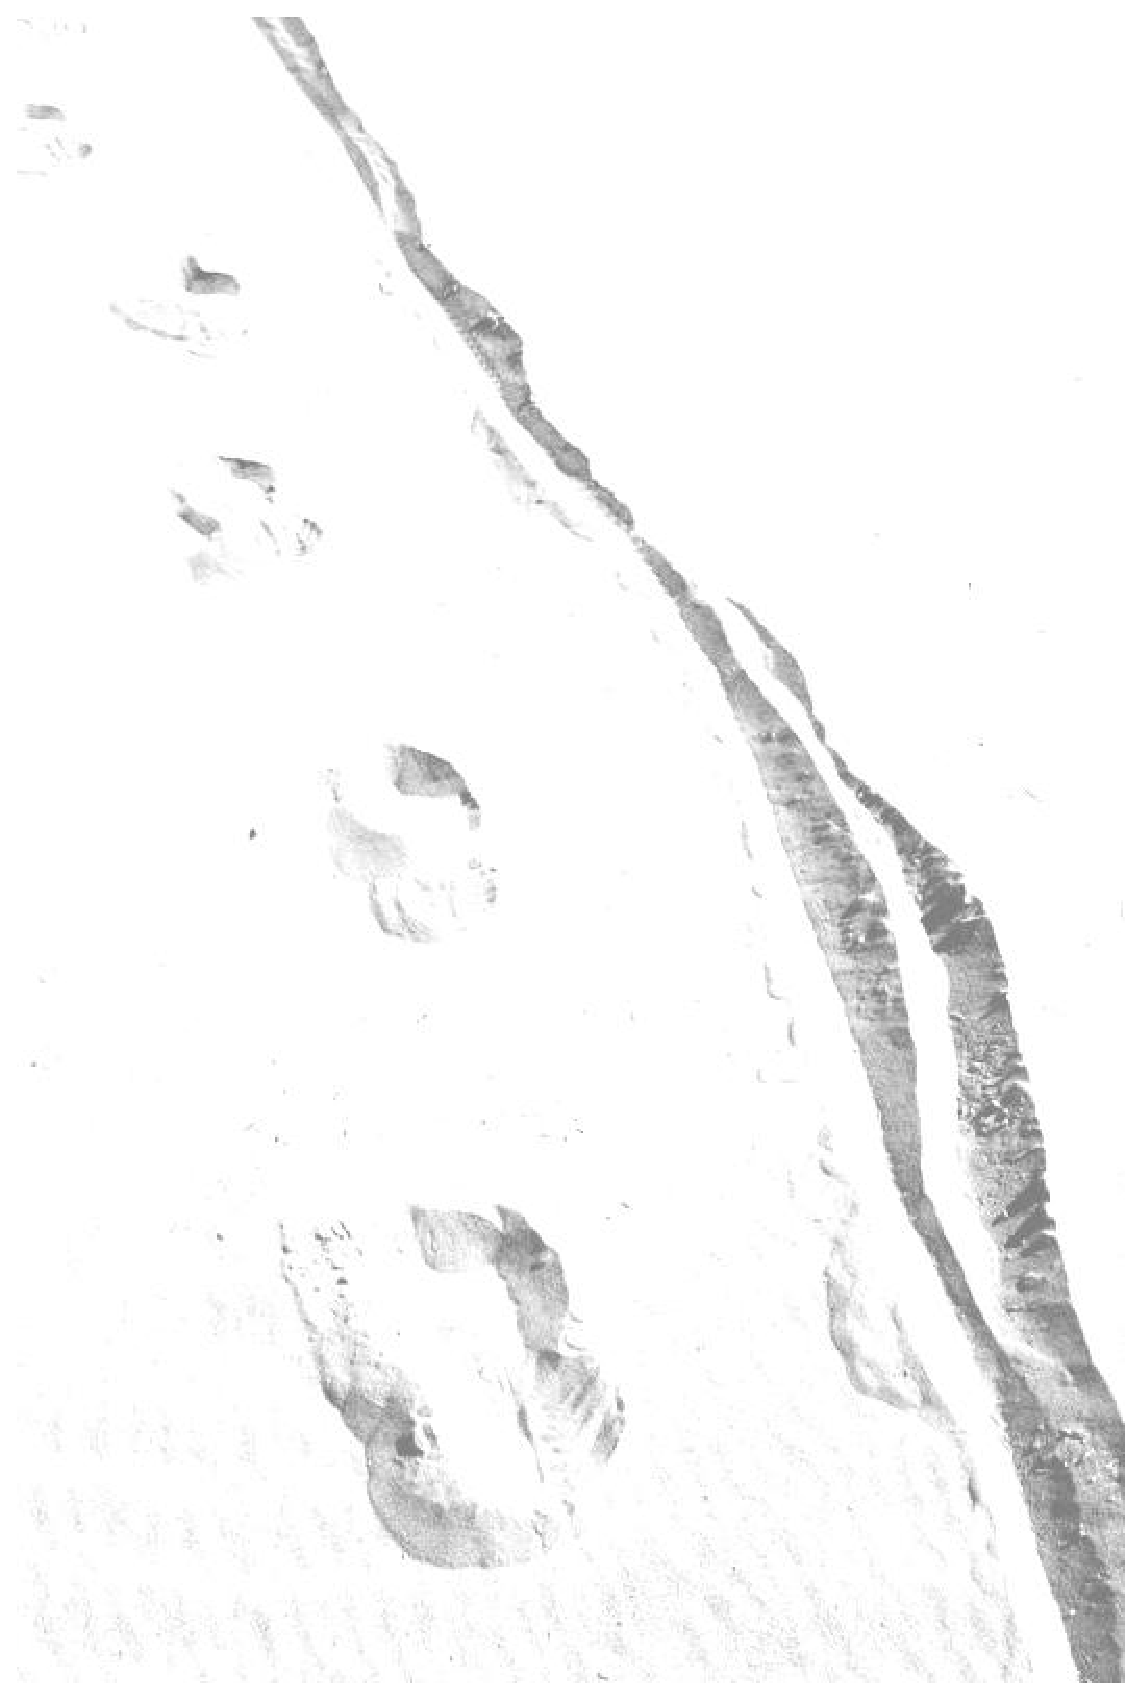
\includegraphics[width=0.55\paperwidth, height = \paperheight]{Figures/Track.eps}}}
  \begin{frame}{\normalsize Outline}
  \tableofcontents[currentsection]
  \end{frame}}
}



\title[AI for Decisions]{AI for Operational Decisions\\ Some perspectives from recent research
}
\author[S. Gros]{\large Prof. Sebastien Gros}
\institute[NTNU]{Department of Cybernetic \\ Faculty of Information Technology \\  NTNU}
\date[Fall 2025]{Freiburg PhD School}


%%%%%%%%%%%%%%%%%%%%%%%%%%%%%%%%%%%%%%%%%%%%%%%%%%%%%%%%%%%%%%%%%%%%%%%%
% Additions for the policy-differentiation part (slides after
% "How to use this more generally? RL over Policy Training")
%%%%%%%%%%%%%%%%%%%%%%%%%%%%%%%%%%%%%%%%%%%%%%%%%%%%%%%%%%%%%%%%%%%%%%%%
\usetikzlibrary{decorations.pathreplacing,fit,backgrounds}
\usepackage{booktabs}

% Overlay-aware TikZ keys: visible on=<2->, onslide=<3->{red}
\tikzset{
  invisible/.style={opacity=0,text opacity=0},
  visible on/.style={alt={#1{}{invisible}}},
  alt/.code args={<#1>#2#3}{\alt<#1>{\pgfkeysalso{#2}}{\pgfkeysalso{#3}}},
  onslide/.code args={<#1>#2}{\only<#1>{\pgfkeysalso{#2}}},
}
% A small quadrotor icon: \pic[<colour, dash>] at (x,y) {drone=<half arm length>};
\tikzset{pics/drone/.style={code={
  \draw[line width=1.1pt] (-#1,0) -- (#1,0);
  \fill[rounded corners=1pt] (-0.17,-0.08) rectangle (0.17,0.08);
  \draw[line width=0.7pt] (-#1,0) -- (-#1,0.12) (#1,0) -- (#1,0.12);
  \draw[fill=white] (-#1,0.15) ellipse (0.24 and 0.045);
  \draw[fill=white] (#1,0.15) ellipse (0.24 and 0.045);
}}}

% Colour code used throughout the new part:
%   red  = MDP parameters theta (simulator, cost, design)
%   blue = policy parameters nu
\newcommand{\mth}{\textcolor{myRed2}{\vect\theta}}
\newcommand{\pnu}{\textcolor{myBlue3}{\vect\nu}}
\newcommand{\nst}{\textcolor{myBlue3}{\vect\nu}^\star}
\newcommand{\kap}{\boldsymbol\kappa}
\newcommand{\sv}{\vect s}
\newcommand{\av}{\vect a}
\newcommand{\Lth}{L_{\mth}}
\newcommand{\rth}{\rho_{\mth}}
\newcommand{\pin}{\pi_{\pnu}}
\newcommand{\Jh}{\hat J_{\mth}}
\newcommand{\Fres}{\vect F}
\newcommand{\E}{\mathbb E}
\newcommand{\Jreal}{J_{\mathrm{real}}}
\definecolor{myOrangeD}{rgb}{0.85,0.42,0.0}
\newcommand{\LR}{\textcolor{myOrangeD}{\textbf{LR}}}
\newcommand{\PD}{\textcolor{myGreen3}{\textbf{PD}}}

%%%%%%%%%%%%%%%%%%%%%%%%%%%%%%%%%%%%%%%%%%%%%%%%%%%%%%%%%%%%%%%%%%%%%%%%

\begin{document}












\begin{frame}{\normalsize Orientation}
\textbf{What we have seen:} 
\begin{itemize}
\footnotesize
\item RLMPC, why does it work \& different flavors
\end{itemize}
\vspace{.5cm}
\visible<2->{
\textbf{What we will do now:} 
\begin{itemize}
\footnotesize
\item The theory is not about MPC, it is about MDPs (MPC is a special case)
\item It has broader implications for AI and model-based decision making
\item Provide (tentative) practical ideas for in Sim2Real
\end{itemize}}
\end{frame} 


{\usebackgroundtemplate{
 \parbox[c][\paperheight][b]{\paperwidth}{
    \flushright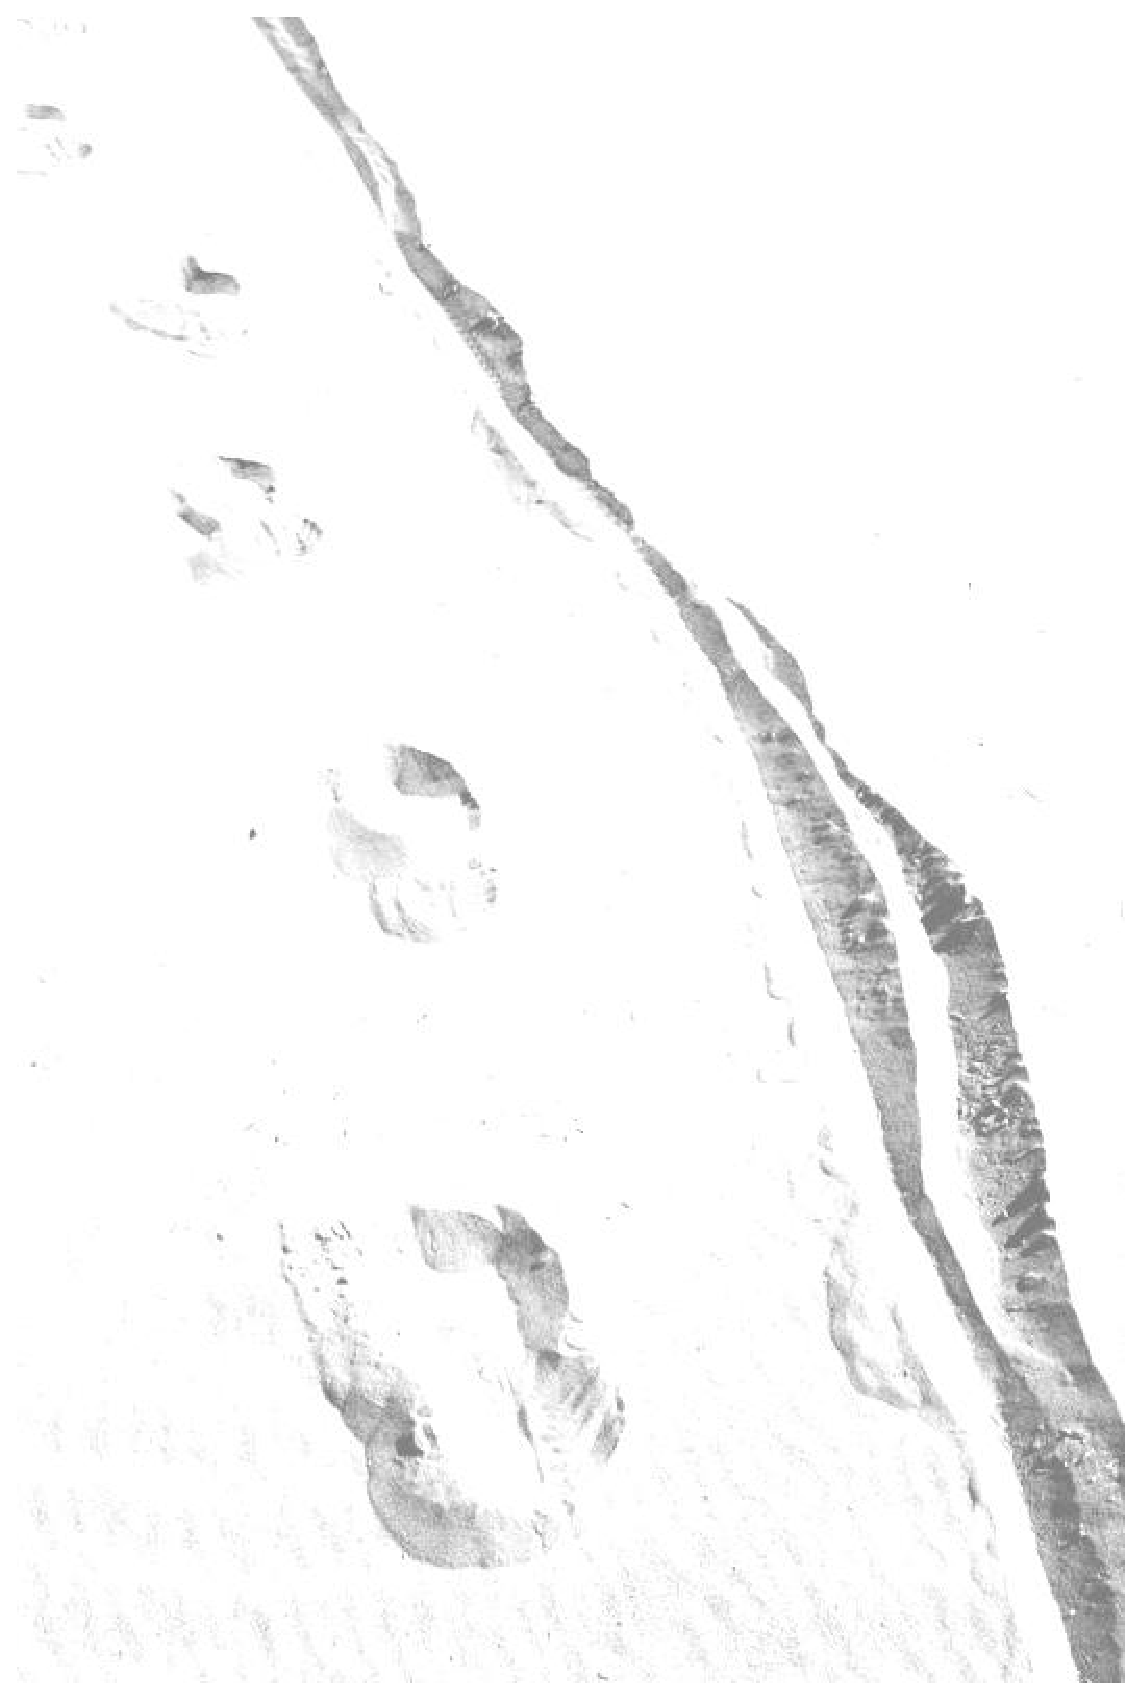
\includegraphics[width=0.55\paperwidth, height = 1\paperheight]{Figures/Track.eps}}}
\begin{frame}
\titlepage
\end{frame}}




%
%\begin{frame}{\normalsize Disclaimer \& Forewords}
%\footnotesize
%\begin{columns}[t]
%\column{0.5\textwidth}
%\textbf{About me} 
%\begin{itemize}
%\item Research in Optimal Control, Markov Decision Processes, Stochastic Optimization, Numerical algorithms, Machine Learning, Reinforcement Learning
%\item Applications in Energy, Energy Economics, Medical Engineering
%\end{itemize}
%
%
%\column{0.5\textwidth}
%\textbf{On this talk}
%\begin{itemize}
%\item This will be a ``high-level" discussion!
%\item Research started in 2018
%\begin{itemize}
%\scriptsize
%\item About 50 papers on the topic
%\item Focused on Reinforcement Learning and MPC, now generalizing
%\end{itemize}
%\item Statistics are underlying everything, great to talk to experts
%\item I will spend time building the background \tiny{(maybe pedestrian, but nothing is ever obvious)}
%\end{itemize}
%\end{columns}
%\vspace{0.25cm}
%\includegraphics[width=1\textwidth,clip]{Figures/SmartGridLab.eps}
%
%\end{frame}

%
%
%\section{Decision making}
%
%\begin{frame}{\normalsize Types of decisions}
%\footnotesize
%\vspace{-.5cm}
%\begin{center}
%\textbf{Focus of this talk is on sequential decision making}
%\end{center}
%\vspace{-.25cm}
%\begin{columns}
%\column{0.7\textwidth}
%\visible<2->{
%\begin{itemize}
%\item At every (discrete) time instant
%\begin{itemize}
%\scriptsize
%\item new information is available
%\item decide of a new action to take on the environment
%\end{itemize}
%\item Information is measurements, forecasts, known future
%\item Rational utility to maximize, guiding the decisions
%\item Actions have ``long-term consequences" on performance
%\item Policy $\vect\pi$ is a function from information  to action
%\item Reality is assumed stochastic
%\end{itemize}
%}
%
%\column{0.3\textwidth}
%
%
%\newcommand{\Sys}{\vspace{-0.25cm}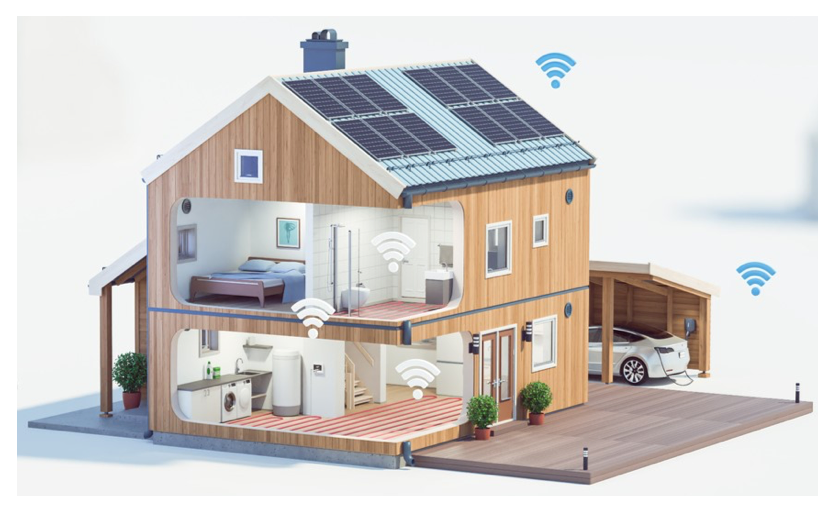
\includegraphics[width=1\textwidth,clip]{Figures/SmartHouse.eps}}
%
%\tikzstyle{Sys_block} = [rectangle, draw, fill=none,  text width=3.cm, text centered, rounded corners, minimum height=4em,inner sep=2pt]
%\tikzstyle{Opt_block} = [rectangle, draw, fill=myLightGreen,  text width=3cm,  text centered, rounded corners]
%\tikzstyle{line} = [draw, -latex']
%
%\begin{tikzpicture}[->,>=stealth']
%
%\node [Sys_block] (sys0) {\Sys};
%
% 
%
% \node [Opt_block, below of=sys0, node distance = 2.7cm] (opt0) {
% \begin{minipage}[c]{3cm}
% \center
%\textbf{Policy} $\vect\pi$\\
%Information to Action
%\end{minipage}
% };
% 
% \path  (sys0) edge[bend left=20]  node[anchor=west] {Information} (opt0)
% (opt0) edge[bend left=20]  node[anchor=east] {Action} (sys0);
%\end{tikzpicture}
%\end{columns}
%
%\vspace{.25cm}
%\visible<3->{
%\textcolor{myBlue2}{\textbf{Ubiquitous problem in our society}}, e.g.
%\begin{itemize}
%\scriptsize
%\item Process control: max revenues, min emissions and wastes / decide on flows, volumes, temperatures
%\item Energy management: min cost of energy / decide on biddings 
%\item Digital healthcare: maximize quality / decide on treatments, clinical pathways
%\item etc.
%\end{itemize}
%}
%
%\visible<4->{\center
%\textbf{Framework to discuss that problem is \textcolor{myRed2}{Markov Decision Processes}}} 
%
%\end{frame}
%
%
%
\section{Decisions from data}
%
%\begin{frame}{\normalsize Markov Decision Processes (MDP)}
%\footnotesize
%\vspace{-.5cm}
%\begin{columns}[t]
%\column{0.49\textwidth}
%\begin{block}{}
%\center
%\textbf{Stochastic state transitions}
%$$\vect s,\vect a\rightarrow \vect s_+$$
%(state-action $\rightarrow$ next state)
%\end{block}
%
%
%
%\column{0.49\textwidth}
%\begin{block}{}
%\center
%\textbf{Utility function} 
%$L(\vect s,\vect a)\in \mathbb R$
%\begin{itemize}
%\item Instantaneous performance
%\item $\infty$ if constraints are violated
%\end{itemize}
%\end{block}
%
%\end{columns}
%
%\begin{columns}[t]
%\column{0.45\textwidth}
%\begin{itemize}
%\item \visible<2->{\textbf{Policy}
%$$\vect a = \vect\pi(\vect s)$$ 
%is how we act on the system}
%\item \visible<3->{ \textbf{Closed-loop performance} 
%\begin{align*}
%J\left(\vect \pi\right) = \mathbb E\left[\left.\sum_{k=0}^\infty \gamma^kL\left(\vect s_k,\vect a_k\right)\,\right|\, \vect a_k = \vect\pi(\vect s_k) \right]
%\end{align*}
%with discount $\gamma \in [0,1]$}
%\item  \visible<4->{ \textbf{Optimal policy}: $\vect \pi^\star$ from
%$$\min_{\vect \pi}\,J\left(\vect \pi\right)$$}
%\end{itemize}
%
%\column{0.45\textwidth}
%
%
%\vspace{-1cm}
%
%%\begin{overlayarea}{\textwidth}{0.25\textheight}
%%\only<1-15>{
%\begin{figure}
%\newcommand{\FS}{.8}
%\begin{overlayarea}{\textwidth}{.4\textheight}
%\only<5>{\includegraphics[width=\FS\textwidth,clip]{Figures/SimpleTrajectories1.eps}}
%\only<6>{\includegraphics[width=\FS\textwidth,clip]{Figures/SimpleTrajectories2.eps}}
%\only<7>{\includegraphics[width=\FS\textwidth,clip]{Figures/SimpleTrajectories3.eps}}
%\only<8>{\includegraphics[width=\FS\textwidth,clip]{Figures/SimpleTrajectories4.eps}}
%\only<9>{\includegraphics[width=\FS\textwidth,clip]{Figures/SimpleTrajectories5.eps}}
%\only<10>{\includegraphics[width=\FS\textwidth,clip]{Figures/SimpleTrajectories6.eps}}
%\only<11>{\includegraphics[width=\FS\textwidth,clip]{Figures/SimpleTrajectories7.eps}}
%\only<12>{\includegraphics[width=\FS\textwidth,clip]{Figures/SimpleTrajectories8.eps}}
%\only<13>{\includegraphics[width=\FS\textwidth,clip]{Figures/SimpleTrajectories9.eps}}
%\only<14>{\includegraphics[width=\FS\textwidth,clip]{Figures/SimpleTrajectories10.eps}}
%\only<15->{\includegraphics[width=\FS\textwidth,clip]{Figures/SimpleTrajectories11.eps}}
%\end{overlayarea}
%\end{figure}
%%}
%\visible<16->{
%\begin{alertblock}{}
%\center
%Decisions at time $k$ taken based on current information $\vect s_k$, knowing that the future is uncertain, and that more information will be available for subsequent decisions
%\end{alertblock}
%}
%%\end{overlayarea}
%
%
%\end{columns}
%
%\end{frame}
%
%\end{document}
%
%
%\begin{frame}{\normalsize Policy from repeated planning (MPC)}
%\footnotesize
%\vspace{-.45cm}
%\begin{center}
%\textbf{Optimize a plan over finite horizon, apply first action, repeat}
%\end{center}
%\vspace{-.75cm}
%\begin{columns}[t]
%\column{0.4\textwidth}
%\begin{block}{}
%\textbf{MPC}: at {\color{blue}current state $\vect s$}
%\vspace{-.5cm}\\
%
%\begin{align*}
%\min_{\vect x,{\color{myGreen3}\vect u}}&\quad  T\left(\vect x_N\right) + \sum_{k=0}^{N-1}\gamma^k L\left(\vect x_k,\vect u_k\right)  \\
%\mathrm{s.t.}&\quad \vect x_{k+1} = \vect f\left(\vect x_k,\vect u_k\right)\\
%%&\quad  \vect h\left(\vect x_k,\vect u_k\right)\leq 0\\
%&\quad \vect{x}_0 = {\color{blue}\vect s}
%\end{align*}
%apply {\color{myGreen3}action $\vect a = \vect u_0^\star$} to the system
%%policy $\vect\pi^\mathrm{MPC}\left(\vect s\right) = {\color{myGreen3}\vect u^\star_{0}}$
%\end{block}
%
%\column{0.6\textwidth}
%\vspace{-.2cm}
%\begin{figure}
%\newcommand{\FS}{.8}
%\begin{overlayarea}{\textwidth}{0.45\textheight}
%\only<1>{\includegraphics[width=\FS\textwidth,clip]{Figures/MPC0.eps}}
%\only<2>{\includegraphics[width=\FS\textwidth,clip]{Figures/MPC1.eps}}
%\only<3>{\includegraphics[width=\FS\textwidth,clip]{Figures/MPC2.eps}}
%\only<4>{\includegraphics[width=\FS\textwidth,clip]{Figures/MPC3.eps}}
%\only<5>{\includegraphics[width=\FS\textwidth,clip]{Figures/MPC4.eps}}
%\only<6>{\includegraphics[width=\FS\textwidth,clip]{Figures/MPC5.eps}}
%\only<7>{\includegraphics[width=\FS\textwidth,clip]{Figures/MPC6.eps}}
%\only<8->{\includegraphics[width=\FS\textwidth,clip]{Figures/MPC7.eps}}
%\end{overlayarea}
%\end{figure}
%\end{columns}
%
%\vspace{.1cm}
%
%\begin{columns}
%\column{0.45\textwidth}
%\visible<9->{
%\begin{block}{}
%\textbf{MPC} 
%\begin{itemize}
%\item is \textbf{based on planning} the future
%\item  \textbf{Policy} from repeated planning $$\vect\pi^\mathrm{MPC}\left(\vect s\right) = {\color{myGreen3}\vect u^\star_{0}}$$
%\end{itemize}}
%\end{block}
%
%\column{0.5\textwidth}
%
%\visible<10->{
%\begin{alertblock}{}
%\textbf{Repeated planning (MPC)}
%\begin{itemize}
%\item Builds a policy for the cost of planning 
%\item Complex relationship \\ ``optimal plan" $\leftrightarrow$ ``optimal policy" 
%\item Stochastic versions exist
%\end{itemize}
%
%\end{alertblock}
%}
%
%\end{columns}
%\visible<11->{
%\center
%\textbf{We will get back to that...}
%}
%
%
%\end{frame}
%
%





\begin{frame}{\normalsize Model-Free Pathway - ``Pure" Reinforcement Learning}
\footnotesize

\newcommand{\Sys}{\vspace{-0.25cm}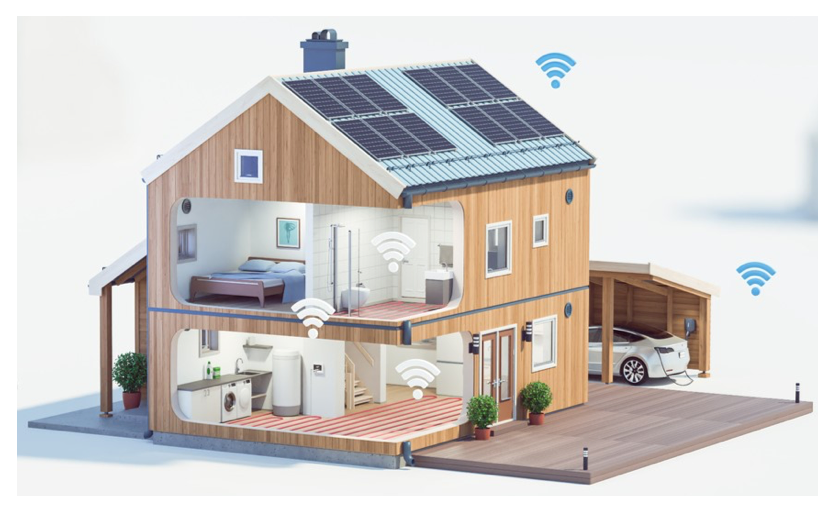
\includegraphics[width=1\textwidth,clip]{Figures/SmartHouse.eps}}

\tikzstyle{Sys_block} = [rectangle, draw, fill=none,  text width=3.cm, text centered, rounded corners, minimum height=4em,inner sep=2pt]
\tikzstyle{Opt_block} = [rectangle, draw, fill=myLightGreen,  text width=3cm,  text centered, rounded corners]
\tikzstyle{RL_block} = [rectangle, draw, fill=myLightBlue,  text width=2.75cm, text centered, rounded corners]    
\tikzstyle{line} = [draw, -latex']

\begin{columns}[t]
\column{0.6\textwidth}



\begin{tikzpicture}[->,>=stealth']

\node [Sys_block] (sys0) {\Sys};

  \visible<2->{
\node [RL_block, left of=sys0, node distance = 4.75cm] (RL0) {
 \begin{minipage}[c]{2.75cm}
\textbf{RL} estimates
\begin{align*}
\nabla_{\vect\theta}J\left(\vect\pi_{\vect \theta}\right)
\end{align*}
\flushright from data
\end{minipage}
 };}
 

 \node [Opt_block, below of=sys0, node distance = 2.7cm] (opt0) {
 \begin{minipage}[c]{3cm}
 \center
\textbf{Policy}
 \vspace{-0.1cm}
\begin{align*}
\vect a = \vect\pi_{\vect \theta}(\vect{s})
\end{align*}

\end{minipage}
 };
 
 
 \path  (sys0) edge[bend left=20]  node[anchor=west] {State} (opt0)
 (opt0) edge[bend left=20]  node[anchor=east] {Actions} (sys0);
 \visible<2->{ \path  (sys0) edge  node[anchor=south] {Real Data} (RL0);}
 \visible<3->{  \path  (RL0) edge[bend right=20]  node[anchor=north east,xshift=0em] {$\vect\theta\leftarrow \vect\theta-\alpha\nabla_{\vect\theta}J\left(\vect\pi_{\vect \theta}\right)$ } (opt0);}
\end{tikzpicture}


\column{0.375\textwidth}
\begin{itemize}
\item Define policy $\vect\pi_{\vect \theta}$ as a parametrized function 
\item Optimize policy as:
\begin{equation*}
\min_{\vect\theta}\,\, J\left(\vect\pi_{\vect \theta}\right)
\end{equation*}
%\item \visible<2->{$\nabla_{\vect\theta}J\left(\vect\pi_{\vect \theta}\right)$ can be estimated from data}
\item \visible<3->{Gradient descent can be used to optimize policy}
\end{itemize} 
\end{columns}
\vspace{.5cm}
 \visible<4->{
\textbf{Remarks}
\begin{itemize}
\item $\vect\pi_{\vect \theta}(\vect{s})$ often from DNN
\item End-to-end training requires a lot of data and effort
\item Difficult to provide explainability and guarantees on the policy we obtain
\item Poor track record of industrial adoption (exception chatbots)
%, generate artificial data that ``look like" reality, etc.
\end{itemize}}
 \visible<5->{\flushright $\rightarrow$policy is often trained on \textcolor{myBlue2}{\textbf{high-fidelity simulations}}: embed knowledge, reduce costs, manage safety, promote explainability, control the training
}

\end{frame}



%\begin{frame}{\normalsize Predictive AI Models}
%\footnotesize
%\begin{center}
%\textbf{``Any tool" turning data into predictions on how reality will evolve}\\ {\scriptsize(My definition, big stretch, I know...)}\\\vspace{.5cm} 
%\textbf{
%\textcolor{myBlue2}{My point will not so much on how we predict but ``what" we predict}
%}
%\end{center}
%
%
%
%\begin{columns}[t]
%\column{0.5\textwidth}
%
%\visible<2->{
%\textbf{Applies to}
%\begin{itemize}
%\item Classic AI tools {\tiny(DNN, LSTM, TFT, etc)}
%\item Statistics of time series
%\item Hybrid modelling
%\item Linear predictors
%\item etc.
%\end{itemize}}
%
%\column{0.5\textwidth}
%
%\visible<3->{
%\textbf{Deliver}
%\begin{itemize}
%\item Probabilistic predictions, e.g.
%\begin{itemize}
%\scriptsize
%\item sampling-based 
%\item scenarios
%\item approximate distribution
%\end{itemize}
%\item Deterministic predictions
%\begin{itemize}
%\scriptsize
%\item distill statistics in ``single-point"
%\item expected value, MLE, etc
%\end{itemize}
%\end{itemize}}
%\end{columns}
%
%
%\end{frame}


\begin{frame}{\normalsize Model-based Pathway - Predictive AI Models \scriptsize{(data-driven, ML, etc)}}
\footnotesize
\vspace{-0.25cm}
\begin{columns}
\column{0.4\textwidth}
\visible<2->{
\begin{block}{\scriptsize One-step model}
\textbf{AI model} e.g.
\vspace{-0.1cm}
\begin{align*}
\hat{\vect{s}}_{k+1} \sim  \rho_{\vect{\theta}}(\cdot\,|\,\vect{s}_k,\vect{a}_k)
\end{align*}
\vspace{-0.75cm}
\flushright fitting data %$\rho$ 
\end{block}
}



\column{0.55\textwidth}
\begin{overlayarea}{\textwidth}{.3\textheight}
\only<1-3>{
\vspace{.4cm} 
\textbf{Real world}: ${\vect{s}}_{k+1} \sim  \rho(\cdot\,|\,\vect{s}_k,\vect{a}_k)$
\vspace{-0.1cm}
\begin{itemize}
\item Data with enough ``richness" 
\end{itemize} 


%\begin{figure}
%\newcommand{\FS}{.8}
%\psfrag{x0}[Bl][Bl][1]{$\vect{s}_k$}
%\psfrag{t}[Bl][Bl][.7]{Time}
%\psfrag{P}[Bl][Bl][1]{$\rho_{\vect\theta}$}
%%\includegraphics[width=\FS\textwidth,clip]{Figures/StatePropagationStochastic.eps}
%\includegraphics[width=\FS\textwidth,clip]{Figures/StatePropagation.eps}
%\end{figure}

}
\only<4->{
\begin{alertblock}{}
\center
Virtual data from ``simulating" $\hat{\vect{s}}_{k+1} \sim  \rho_{\vect{\theta}}(\cdot\,|\,\vect{s}_k,\vect{a}_k)$ forward (Monte Carlo)
\end{alertblock}
\vspace{-.25cm}
}
\visible<5->{
\begin{alertblock}{}
\center
In most cases, $\rho_{\vect{\theta}}$ is a fairly simple representation of reality $\rho$, easy to sample from
\end{alertblock}
 }
\end{overlayarea}


\end{columns}
\vspace{-.2cm}
\visible<2->{
\begin{center}
\textit{Here we no longer need the model $\rho_{\vect{\theta}}$ to be ``optimization-friendly"}
\end{center}
}
%\vspace{.2cm}
%\begin{overlayarea}{\textwidth}{.5\textheight}
%\only<3-5>{
\visible<3->{
\textbf{Model parameters $\vect\theta$}
\begin{itemize}
\item Selected such that model $\rho_{\vect{\theta}}$ ``ressembles" reality $\rho$, using data (+ physics)
\item Deterministic models are a special case of $\rho_{\vect{\theta}}$
\item Many methods, from Least Squares and MLE to Bayesian and Adversarial Learning
\item Still, in most cases $\rho_{\vect{\theta}}$ ``simplifies" $\rho$ because
\begin{itemize}
\scriptsize
\item need for huge amounts of data to decide $\vect\theta$ if model is very rich
\item computationally demanding simulations if $\rho_{\vect{\theta}}$ is expensive to sample from
\end{itemize}
\item Then
\begin{itemize}
\scriptsize
\item biases in case of insufficiently rich model structure
\item validity is limited to some parts of the state-action space
\item only few first moments are correct (typ. mean + variance)
\end{itemize}
\end{itemize}}


\end{frame}


\begin{frame}{\normalsize Back to MPC - A ``Classical" View on Decision Making}
\footnotesize
\begin{columns}
\column{0.45\textwidth}
\begin{block}{}
\textbf{Policy} $\vect\pi_{\vect \theta}(\vect{s})$ given implicitly by 
\vspace{-.5cm}\\
\begin{align*}
\min_{\vect x,{\color{myGreen3}\vect u}}&\quad  \mathbb E\left[ T\left(\vect x_N\right) + \sum_{k=0}^{N-1} L\left(\vect x_k,\vect u_k\right) \right] \\
\mathrm{s.t.}&\quad \vect x_{k+1} \sim \rho_{\vect\theta}\left(\vect x_k,\vect u_k\right)\\
%&\quad  \vect h\left(\vect x_k,\vect u_k\right)\leq 0\\
&\quad \vect{x}_0 = {\color{blue}\vect s}
\end{align*}
\flushright use $\vect\pi_{\vect \theta}(\vect{s}) = {\color{myGreen3}\vect u_0^\star}$ on the system
\end{block}

\column{0.525\textwidth}
\vspace{-0.3cm}
\begin{overlayarea}{\textwidth}{0.3\textheight}
\only<3>{
\begin{alertblock}{}
\textbf{\textcolor{black}{Defines a paradigm}}...\\
\vspace{0.1cm}
\begin{itemize}
\item Performance from model accuracy
$$\text{i.e. }\rho_{\vect\theta}\text{ ``close enough" to }\rho$$
\item ``Ignore" that we replan all the time
\end{itemize}
\end{alertblock}
}
\only<4->{

\textbf{Relationship $\vect\pi_{\vect\theta}$ to $\vect\pi^\star$??}
\begin{itemize}
\scriptsize
\item They match if $\rho_{\vect{\theta}}$ is exact and deterministic
\item But it usually cannot be...
\end{itemize}
 \vspace{-0.3cm}
\visible<5->{
\begin{alertblock}{}
\center\textbf{
``Standard methods" for choosing $\vect \theta$ in general do not yield the best $\vect\pi_{\vect \theta}$.\\
RL over MPC can fix that, $L$ becomes part of the model}
\end{alertblock}
}}
\end{overlayarea}




\end{columns}

\newcommand{\Sys}{\vspace{-0.25cm}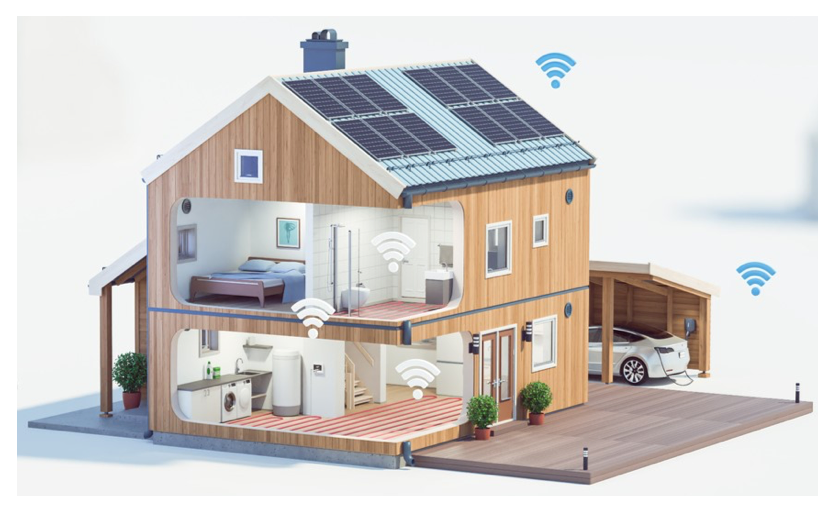
\includegraphics[width=1\textwidth,clip]{Figures/SmartHouse.eps}}

\tikzstyle{Sys_block} = [rectangle, draw, fill=none,  text width=3.cm, text centered, rounded corners, minimum height=4em,inner sep=2pt]
\tikzstyle{Opt_block} = [rectangle, draw, fill=myLightGreen,  text width=2.85cm,  text centered, rounded corners]
\tikzstyle{ID_block} = [rectangle, draw, fill=myLightBlue,  text width=3cm, text centered, rounded corners]    
\tikzstyle{line} = [draw, -latex']

\begin{tikzpicture}%[node distance = 4cm, auto]

\node [Sys_block] (sys0) {\Sys};
\node [Opt_block, left of=sys0, node distance = 4cm] (opt0) {
 \begin{minipage}[c]{2.75cm}
 \center
\textbf{MPC policy}
 \vspace{-0.1cm}
\begin{align*}
\vect\pi_{\vect \theta}(\vect{s})
\end{align*}
\textbf{from model}
\begin{align*}
\vect{s}_{k+1} \sim {\rho}_{\vect{\theta}}(.\,|\,\vect{s}_k,\vect{a}_k)
\end{align*}
\end{minipage}
 };
 
\visible<2->{
\node [ID_block, right of=sys0, node distance = 4.75cm] (ID0) {
 \begin{minipage}[c]{3cm}
\textbf{AI model} 
\begin{align*}
\hat{\vect{s}}_{+} \sim \rho_{\vect{\theta}}\left(\cdot\,|\,\vect{s},\vect{a}\right)
\end{align*}
\vspace{-.75cm}
\flushright fitting data $\rho$
\end{minipage}
 };
%\node [ID_block, right of=sys0, node distance = 4.5cm] (ID0) {
% \begin{minipage}[c]{3.0cm}
%\center
%\textbf{AI model} adjust ${\vect{\theta}}$ to fit model ${\rho}_{\vect{\theta}}$ to data $\vect{s}_k,\vect{a}_k,\vect{s}_{k+1}$
%\end{minipage}
% }; 
 }
\path [line] (opt0) -- node [ anchor=south] {$\vect{a}$} (sys0);
\path [line] (sys0.south)  -- ++(0,-0.5) -| node [ anchor=north] {$\vect{s}$} (opt0.south);
\visible<2->{\path [line] (sys0) -- node [ anchor=center,xshift=-.5em] { \begin{minipage}[c]{1cm}
  \center
 Data\\ knowledge
 \end{minipage}} (ID0);}
\visible<2->{\path [line] (ID0.north) -- ++(0,0.6) -| node [ anchor=south] {${\vect{\theta}}$} (opt0.north);}
 \end{tikzpicture}
 \vspace{-.25cm}
\center
\visible<6->{\textbf{This is not the only way of taking decisions from models}}
\end{frame}




\begin{frame}{\normalsize Decision policy from AI models (Sim2Real)}
\footnotesize


\newcommand{\Sys}{\vspace{-0.25cm}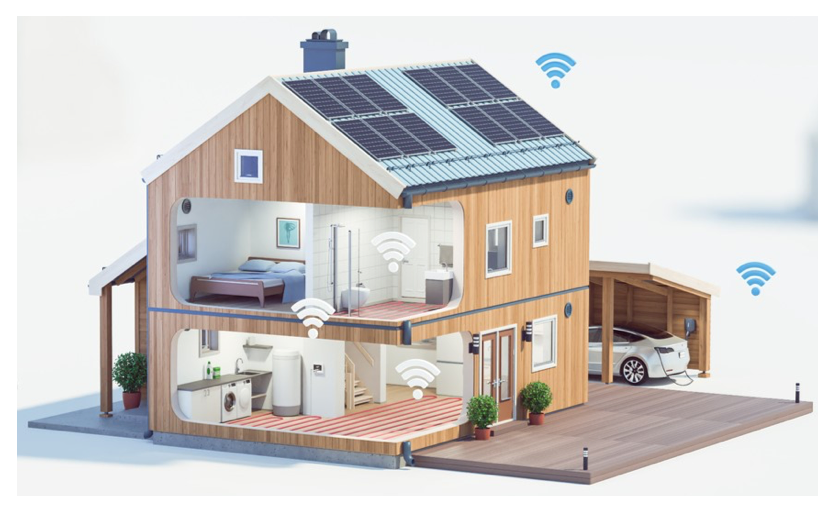
\includegraphics[width=1\textwidth,clip]{Figures/SmartHouse.eps}}

\tikzstyle{Sys_block} = [rectangle, draw, fill=none,  text width=3.cm, text centered, rounded corners, minimum height=4em,inner sep=2pt]
\tikzstyle{Obj_block} = [rectangle, draw, fill=myLightRed,  text width=2.7cm, text centered, rounded corners, minimum height=4em,inner sep=2pt]
\tikzstyle{Opt_block} = [rectangle, draw, fill=myLightGreen,  text width=3cm,  text centered, rounded corners]
\tikzstyle{ID_block} = [rectangle, draw, fill=myLightBlue,  text width=3cm, text centered, rounded corners]    
\tikzstyle{line} = [draw, -latex']

\begin{tikzpicture}[->,>=stealth']

\node [Sys_block] (sys0) {\Sys};

\node [ID_block, left of=sys0, node distance = 5cm] (ID0) {
 \begin{minipage}[c]{3cm}
\textbf{AI model} 
\begin{align*}
\hat{\vect{s}}_{+} \sim \rho_{\vect{\theta}}\left(\cdot\,|\,\vect{s},\vect{a}\right)
\end{align*}
\vspace{-.75cm}
\flushright fitting data $\rho$
\end{minipage}
 };


 \visible<2->{
 \node [Opt_block, below of=ID0, node distance = 2.5cm] (opt0) {
 \begin{minipage}[c]{3cm}
 \center
\textbf{Policy}
 \vspace{-0.2cm}\\
 \begin{overlayarea}{\textwidth}{0.1\textheight}
\only<1-4>{
 \vspace{-0.2cm}
\begin{align*}
\vect a=\vect \pi_{\vect \nu}(\vect{s})
\end{align*}
}
\only<5->{
 \vspace{-0.2cm}
\begin{align*}
\vect a=\vect \pi_{\vect \theta}(\vect{s})
\end{align*}}
\end{overlayarea}
optimal for AI model
\end{minipage}
 };}
 
 \visible<2->{
 \node [Obj_block, left of=opt0, node distance = 4cm] (Obj0) {
 \begin{minipage}[c]{2.7cm}
\textbf{Objective}
\vspace{-.5cm}\\
\begin{align*}
L\left(\vect s,\vect a\right)
\end{align*}
\vspace{-0.8cm}
\flushright possibly unbounded
\end{minipage}
 };}
 
 \path 
 (sys0) edge  node[anchor=center,xshift=-.5em] {
  \begin{minipage}[c]{1cm}
  \center
 Data\\ knowledge
 \end{minipage}} (ID0);
 
\visible<2->{ \path  (ID0) edge[bend left=20]  node[anchor=west] {Virtual data} (opt0);}
\visible<2->{ \path   (opt0) edge[bend left=20]  node[anchor=east] {Actions} (ID0);}
\visible<3->{ \path  (opt0) edge[bend right=20]  node[anchor=west,xshift=1em] {Policy} (sys0);}
\visible<2->{ \path  (Obj0) edge  node[anchor=south] {Cost} (opt0) ;}
\end{tikzpicture}



\begin{overlayarea}{\textwidth}{0.45\textheight}
\only<1-4>{\visible<1-4>{
\vspace{-.25cm}
\textbf{Classical Process:}}
\begin{itemize}
\item \visible<1-4>{Fit AI model $\rho_{\vect\theta}$ to real data}
\item \visible<2-4>{Develop optimal policy for $L$ and $\rho_{\vect\theta}$ from AI model, e.g. using In-Sim RL
\begin{itemize}
\scriptsize
\item Define parametrized policy $\vect\pi_{\vect\nu}$
\item Optimize policy parameters $\vect\nu$ for performance w.r.t. AI model: $\rho_{\vect\theta},L\,\rightarrow\,\vect\nu^\star$
\end{itemize}}
\item \visible<3-4>{Transfer policy $\vect\pi_{\vect\nu^\star}$ into the real world}
\end{itemize}
%\vspace{-.4cm}
\center
\visible<4>{\textbf{Note: policy parameters $\vect\nu^\star$ optimal for AI model become function of $\vect\theta$ \\ Let's then label $\vect\pi_{\vect\theta} = \vect\pi_{\vect\nu^\star}$ for simplicity}}
}
\only<5->{
\textbf{Remarks}
\begin{itemize}
\scriptsize
\item Relationship $\vect\pi_{\vect\theta}$ to $\vect\pi^\star$??
\begin{itemize}
\scriptsize
\item They match if $\rho_{\vect{\theta}}=\rho$, i.e. if model is exact
\item But $\rho_{\vect{\theta}}$ is (almost always) an approximation
\end{itemize}
\end{itemize}}
 \vspace{-0.3cm}
\visible<6->{
\begin{alertblock}{}
\center
\textbf{Are ``standard methods" for choosing $\vect \theta$ resulting in a good policy $\vect\pi_{\vect \theta}$?? Empirically the answer is ``no". Then how to choose $\vect \theta$ to get a good policy?}
\end{alertblock}
}


\end{overlayarea}

\end{frame}

\begin{frame}{\normalsize MPC or Sim2Real - It's the same question...}
\footnotesize
\vspace{-.1cm}
\visible<2->{
\begin{center}
\textit{The theory is about model-based decisions, and equivalences between MDPs}
\end{center}}
\vspace{-.6cm}
\begin{columns}[t]
\column{0.49\textwidth}
\visible<3->{
\begin{block}{\footnotesize \textcolor{myRed}{World} \textcolor{black}{MDP}}
\textbf{World MDP definition} 
\begin{itemize}
\item States $\vect s$ and actions $\vect a$
\item Cost $\textcolor{myRed}{L}\left(\vect s,\vect a\right)$
\item Transition $\vect s_+\sim\textcolor{myRed}{\rho}\left[\,\cdot\,|\vect s,\vect a\right]$
\end{itemize}
\visible<4->{
\textbf{Optimal value functions}
\vspace{-.1cm}
\begin{align*}
V^\star\left(\vect s\right) &= \min_{\vect a}\,Q^\star\left(\vect s,\vect a\right) \\
Q^\star\left(\vect s,\vect a\right)&= \textcolor{myRed}{L}\left(\vect s,\vect a\right)+\gamma \mathbb E_{\vect s_+\sim\textcolor{myRed}{\rho}}\left[V^\star\left(\vect s_+\right)|\vect s,\vect a\right]\\
\end{align*}}
\vspace{-1cm}\\
\visible<5->{
\textbf{Optimal policy}
\vspace{-0.2cm}
\begin{align*}
\vect\pi^\star\left(\vect s\right)=\argmin_{\vect a}\,Q^\star\left(\vect s,\vect a\right)
\end{align*}}
\vspace{-.4cm}
\end{block}}
\column{0.001\textwidth}
\column{0.49\textwidth}
\visible<6->{
\begin{block}{\footnotesize \textcolor{myBlue2}{Model} \textcolor{black}{MDP (simulation environment)}}
\textbf{Model MDP definition} 
\begin{itemize}
\item States $\vect s$ and actions $\vect a$
\item Cost $\textcolor{myBlue2}{\hat L}\left(\vect s,\vect a\right)$
\item Transition $\vect s_+\sim\textcolor{myBlue2}{\hat \rho}\left[\,\cdot\,|\vect s,\vect a\right]$
\end{itemize}
\visible<6->{
\textbf{Optimal value functions}
\vspace{-.1cm}
\begin{align*}
\hat V^\star\left(\vect s\right) &= \min_{\vect a}\,\hat Q^\star\left(\vect s,\vect a\right) \\
\hat Q^\star\left(\vect s,\vect a\right)&= \textcolor{myBlue2}{\hat L}\left(\vect s,\vect a\right)+\gamma \mathbb E_{\vect s_+\sim\textcolor{myBlue2}{\hat\rho}}\left[\left.\,V^\star\left(\hat{\vect s}_+\right)\right|\,\vect s,\vect a\right]\\
\end{align*}}
\vspace{-1cm}\\
\visible<6->{
\textbf{Optimal policy}
\vspace{-0.2cm}
\begin{align*}
\hat{\vect\pi}^\star\left(\vect s\right)=\argmin_{\vect a}\,\hat Q^\star\left(\vect s,\vect a\right)
\end{align*}}
\vspace{-.4cm}
\end{block}}
\end{columns}
\visible<7->{
\begin{alertblock}{}
\vspace{-.1cm}
\center \textbf{Theory says} that - under some technical conditions - there is a $\textcolor{myBlue2}{\hat L}$ such that $\hat Q^\star = Q^\star$
\end{alertblock}}
\visible<8->{
\underline{Proof}: telescopic sum, some non-trivial assumptions to prevent $\infty-\infty$ cancellations}
\end{frame}


\begin{frame}{\normalsize More on MDP Equivalence}
\footnotesize
\vspace{-.25cm}
\begin{columns}[t]
\column{0.49\textwidth}
\begin{block}{\footnotesize \textcolor{myRed}{World} \textcolor{black}{MDP}}
\begin{itemize}
\item States $\vect s$ and actions $\vect a$
\item Cost $\textcolor{myRed}{L}\left(\vect s,\vect a\right)$
\item Transition $\vect s_+\sim\textcolor{myRed}{\rho}\left[\,\cdot\,|\vect s,\vect a\right]$
\end{itemize}
\end{block}
\column{0.001\textwidth}
\column{0.49\textwidth}

\begin{block}{\footnotesize \textcolor{myBlue2}{Model} \textcolor{black}{MDP}}
\begin{itemize}
\item States $\vect s$ and actions $\vect a$
\item Cost $\textcolor{myBlue2}{\hat L}\left(\vect s,\vect a\right)$
\item Transition $\vect s_+\sim\textcolor{myBlue2}{\hat \rho}\left[\,\cdot\,|\vect s,\vect a\right]$
\end{itemize}
\end{block}


\end{columns}

\visible<2->{
\begin{alertblock}{}
\vspace{-.1cm}
\textbf{Theory says} that 
\vspace{-.1cm}
\begin{itemize}
\scriptsize
\item Under some technical conditions there is a $\textcolor{myBlue2}{\hat L}$ such that $\hat Q^\star = Q^\star$
\item \visible<3->{For $\textcolor{myBlue2}{\hat L}=L$ there is a (non-unique) ``optimal" model $\textcolor{myBlue2}{\hat\rho}$ such that $\hat Q^\star = Q^\star$}
\item \visible<4->{Conditions for model $\textcolor{myBlue2}{\hat\rho}$ ``optimality" $\neq$ min of classical loss functions (except. LQR)}
\item \visible<5->{World MDP and Model MDP do not need to use the same discount $\gamma$}
\end{itemize}
\end{alertblock}}
\vspace{.25cm}
\begin{overlayarea}{\textwidth}{0.5\textheight}
\only<6>{
\textbf{In-Sim policy training uses a Model MDP}
\begin{itemize}
\scriptsize
\item Practitioners mostly work on model $\textcolor{myBlue2}{\hat \rho}$, but ``unsure" on how to tune it
\item In the ML communities, people talk about ``value alignment", we are trying to make this ``MDP equivalence" understood
%\item Finite horizon: ok if correct terminal cost
%\item Scenario tree: rough $\textcolor{myGreen2}{\hat \rho}$
\end{itemize}
}
\only<7->{
\vspace{-.5cm}
\begin{columns}
\column{0.725\textwidth}
\textbf{Remarks}
\begin{itemize}
\scriptsize
\item Non-unique optimal model $\textcolor{myBlue2}{\hat \rho}$ leaves room for aligning it to the real world (classical fitting)
\item \visible<8->{If $V^\star$ is continuous and support of $\textcolor{myRed}{\rho}$ is bounded(?) and path-connected, then we can have support $\textcolor{myBlue2}{\hat \rho}$ $\subset$ support of  $\textcolor{myRed}{\rho}$ }
\item \visible<11->{\textit{More simply said}: we can build optimal models $\textcolor{myBlue2}{\hat \rho}$ that make ``plausible" predictions about the real world.}
\end{itemize}
\column{0.275\textwidth}
\begin{overlayarea}{\textwidth}{0.33\textheight}
\only<9>{
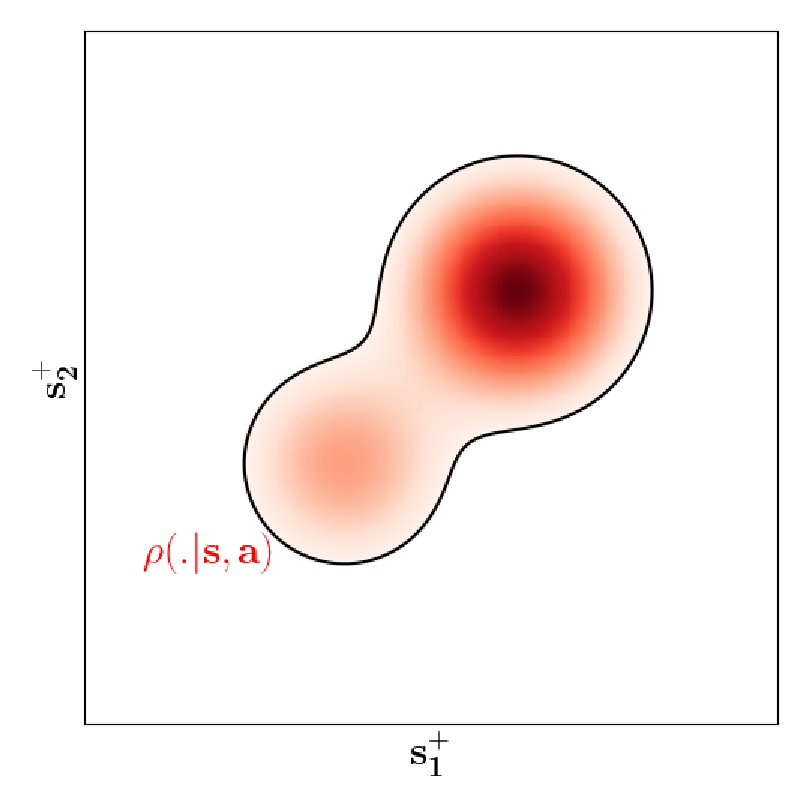
\includegraphics[width=1\textwidth,clip]{Codes/MDPEquivalence/World.eps}
}
\only<10->{
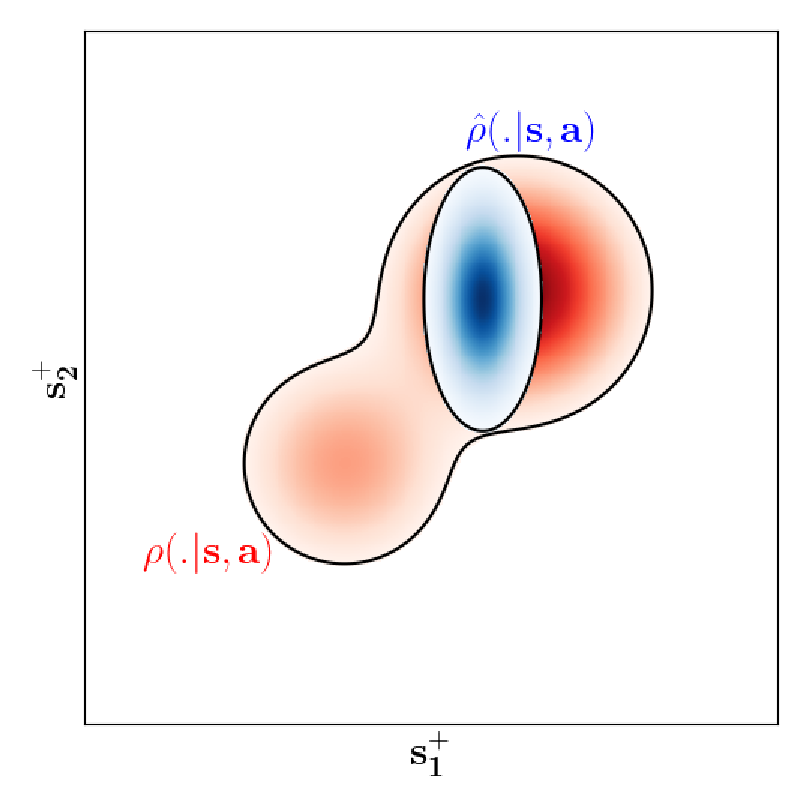
\includegraphics[width=1\textwidth,clip]{Codes/MDPEquivalence/Model.eps}
}
\end{overlayarea}

\end{columns}
}

\end{overlayarea}


\end{frame}
%
%\begin{frame}{\normalsize Is there a catch? A side track...}
%\footnotesize
%\vspace{-1cm}
%\begin{columns}[t]
%\column{0.49\textwidth}
%\begin{block}{\footnotesize \textcolor{myRed}{World} \textcolor{black}{MDP}}
%\begin{itemize}
%\item States $\vect s$ and actions $\vect a$
%\item Cost $\textcolor{myRed}{L}\left(\vect s,\vect a\right)$
%\item Transition $\vect s_+\sim\textcolor{myRed}{\rho}\left[\,\cdot\,|\vect s,\vect a\right]$
%\end{itemize}
%\end{block}
%\column{0.001\textwidth}
%\column{0.49\textwidth}
%
%\begin{block}{\footnotesize \textcolor{myBlue2}{Model} \textcolor{black}{MDP}}
%\begin{itemize}
%\item States $\vect s$ and actions $\vect a$
%\item Cost $\textcolor{myBlue2}{\hat L}\left(\vect s,\vect a\right)$
%\item Transition $\vect s_+\sim\textcolor{myBlue2}{\hat \rho}\left[\,\cdot\,|\vect s,\vect a\right]$
%\end{itemize}
%\end{block}
%
%
%\end{columns}
%\begin{alertblock}{}
%\vspace{-.1cm}
%\center \textbf{Theory says} that - under some technical conditions - there is a $\textcolor{myBlue2}{\hat L}$ such that $\hat Q^\star = Q^\star$
%\end{alertblock}
%\vspace{.25cm}
%\begin{overlayarea}{\textwidth}{0.3\textheight}
%\only<2-4>{
%\textbf{But we are making a strong assumption} (in plain sight)
%\visible<3->{
%\begin{itemize}
%\item Theory assumes that World MDP and Model MDP have the same state $\vect s$
%\item I.e. we need to know the state of the World MDP to build a correct Model MDP
%\item That is often impossible...
%\end{itemize}}
%\flushright\visible<4->{\textbf{The end of a nice theory? No, but it is a word of caution...}}
%}
%\only<5->{\textbf{Eventually the Markov state $\vect s$ boils down to the history of past observations}
%\vspace{-.25cm}
%\begin{flushright}\textit{How to embed that in a model?}\end{flushright}
%\vspace{-.35cm}
%\begin{enumerate}
%\item \visible<6->{``Input-output models": ARX, multi-step predictors (more in a bit), etc.}
%\item \visible<7->{Latent states (a.k.a. embeddings or compressed representations) giving an AI-driven lower-dimensional version of that history}
%\item \visible<8->{State observers giving a model-based lower-dimensional version of that history (more in next slide)}
%\end{enumerate}
% \visible<9->{\center Options 2 and 3 are part of the decision-making process, back-propagate through policy + state ``constructor". }
%}
%\end{overlayarea}
%\end{frame}
%
%\begin{frame}{\normalsize State Estimation in the Learning Loop}
%\footnotesize
%
%\newcommand{\Sys}{\vspace{-0.25cm}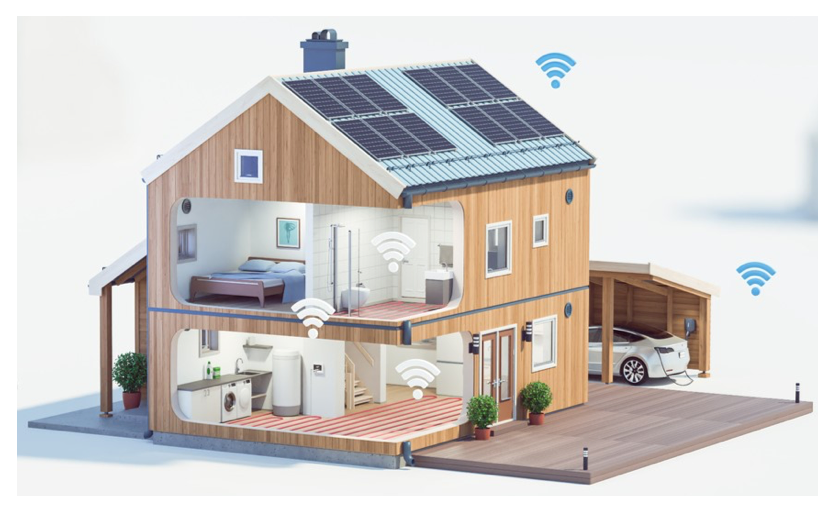
\includegraphics[width=1\textwidth,clip]{Figures/SmartHouse.eps}}
%
%\tikzstyle{Sys_block} = [rectangle, draw, fill=none,  text width=2.5cm, text centered, rounded corners, minimum height=4em,inner sep=2pt]
%\tikzstyle{Opt_block} = [rectangle, draw, fill=myLightGreen,  text width=2cm,  text centered, rounded corners]
%\tikzstyle{ID_block} = [rectangle, draw, fill=myLightBlue,  text width=2.5cm, text centered, rounded corners]    
%\tikzstyle{Obs_block} = [rectangle, draw, fill=myLightRed,  text width=2cm, text centered, rounded corners]    
%\tikzstyle{line} = [draw, -latex']
%
%\begin{tikzpicture}%[node distance = 4cm, auto]
%
%\node [Sys_block] (sys0) {\Sys};
%
%\node [Opt_block, left of=sys0, node distance = 3cm] (opt0) {
% \begin{minipage}[c]{2cm}
% \center
%\textbf{\footnotesize Policy} 
% \vspace{-.1cm}
%$$\vect\pi_{\textcolor{myGreen3}{\vect\theta}}\left({\color{blue}\vect s} \right)$$
%\end{minipage}
% };
%
%\visible<2->{
%\node [Obs_block, below of=opt0, node distance = 1.75cm] (obs0) {
% \begin{minipage}[c]{2cm}
% \center
%\textbf{\footnotesize State estimation} 
% \vspace{-.25cm}
%$${\color{blue}\vect s} = \varphi_{\textcolor{myGreen3}{\vect\theta}}\left(\text{\textcolor{myRed2}{Data}}\right)$$
%%$$\text{Data}\xrightarrow[]{\textcolor{myGreen3}{\vect\theta}} {\color{blue}\vect s}$$
%\end{minipage}
% };
%}
% 
%\node [ID_block, right of=sys0, node distance = 4.2cm] (ID0) {
% \begin{minipage}[c]{2.5cm}
%\textbf{RL} estimates
%\begin{align*}
%\nabla_{\textcolor{myGreen3}{\vect\theta}}J\left(\vect\pi_{\textcolor{myGreen3}{\vect\theta}}\right) 
%\end{align*}
%\flushright from data
%\end{minipage}
% };
% 
%  \visible<3->{
%  \draw[blue,thick] ($(opt0.north east)+(+0.15,0.15)$)  rectangle ($(obs0.south west)+(-0.15,-0.15)$);
%  }
%  
%  
%\path [line] (opt0) -- node [ anchor=south] {$\vect{a}$} (sys0);
%\visible<1>{\path [line] (sys0.south)  -- ++(0,-.5) -| node [ anchor=north] {${\color{blue}\vect s}$} (opt0.south);}
%\path [line] (sys0) -- node [ anchor=south] {\textcolor{myRed2}{Data}} (ID0);
%\path [line] (ID0.north) -- ++(0,0.25) -| node [ anchor=east] {$\textcolor{myGreen3}{\vect\theta}$} (opt0.north);
%
%\visible<2->{\path [line] (sys0.south)   |- node [ anchor=north] {\textcolor{myRed2}{Data}} (obs0.east);}
%\visible<2->{\path [line] (obs0.north)  -- node [ anchor=west] {${\color{blue}\vect s}$} (opt0.south);}
%
%  \visible<3->{
%\path [line] (ID0.south)  -- ++(0,-2) -| node [ anchor=north] {$\textcolor{myGreen3}{\vect\theta}$} (obs0.south);
%  }
%
% \end{tikzpicture}
% 
%
%
%
%
%\begin{columns}
%\column{0.65\textwidth}
%
%\begin{overlayarea}{\textwidth}{0.5\textheight}
%\only<4-6>{
%
%\textbf{Remarks}
%\begin{itemize}
%\scriptsize
%%\item State Estimation (SE) gives ${\color{blue}\vect s} = \varphi_{\textcolor{myGreen3}{\vect\theta}}\left(\text{\textcolor{myRed2}{Data}}\right)$
%\item \visible<4->{Policy is ${\vect\pi}^\text{D}_{\textcolor{myGreen3}{\vect\theta}}\left(\text{\textcolor{myRed2}{Data}}\right) = \vect\pi_{\textcolor{myGreen3}{\vect\theta}}\left(\varphi_{\textcolor{myGreen3}{\vect\theta}}\left(\text{\textcolor{myRed2}{Data}}\right)\right)$}
%\item \visible<5->{Gradient of the policy now is:
%\begin{align*}
%\nabla_{\textcolor{myGreen3}{\vect\theta}} {\vect\pi}^\text{D}_{\textcolor{myGreen3}{\vect\theta}}\left(\text{\textcolor{myRed2}{Data}}\right) = \nabla_{\textcolor{myGreen3}{\vect\theta}}\vect\pi_{\textcolor{myGreen3}{\vect\theta}}\left({\color{blue}\vect s}\right) + \nabla_{\textcolor{myGreen3}{\vect\theta}}\varphi_{\textcolor{myGreen3}{\vect\theta}}\left(\text{\textcolor{myRed2}{Data}}\right) \nabla_{{\color{blue}\vect s}}\vect\pi_{\textcolor{myGreen3}{\vect\theta}}\left({\color{blue}\vect s}\right)
%\end{align*}}
%\vspace{-.5cm}
%\item \visible<6->{Critic is looking at $\text{\textcolor{myRed2}{Data}}\xrightarrow[]{\textcolor{myGreen3}{\vect\theta}} \vect a$, i.e. $Q^{{\vect\pi}^\text{D}_{\textcolor{myGreen3}{\vect\theta}}}\left(\text{\textcolor{myRed2}{Data}},\vect a\right)$}
%\end{itemize}
%
%}
%
%\only<7->{
%\textbf{If $\varphi_{\textcolor{myGreen3}{\vect\theta}}\left(\text{\textcolor{myRed2}{Data}}\right)$ is}
%\begin{itemize}
%\scriptsize
%\item MHE, then its gradient is computed using NLP sensitivities (same as MPC)
%\item DNN, then efficient sensitivity computations exist
%\item Bayesian inference? Belief state? Open research topic...
%\end{itemize}
%}
%
%
%\end{overlayarea}
%
%\column{0.35\textwidth}
%\vspace{-1cm}
%\visible<8->{
%\includegraphics[width=1\textwidth,clip,trim= 0 0 0 0]{Figures/RL_BL_TD}
%}
%
%
%\end{columns}
%
%
%	
%
%
%\end{frame}
%
%\begin{frame}{\normalsize Multi-Step Predictive Control}%: RL for Data-driven Input-Output Multi-steps Predictors}
%\footnotesize
%\begin{columns}
%\column{0.35\textwidth}
%%\vspace{-0.5cm}
%\begin{overlayarea}{\textwidth}{0.55\textheight}
%\only<1-2>{
%
%\textbf{Systems with}
%\begin{itemize}
%\item $\sim$Linear dynamics
%\item Input-output data
%\item Significant stochasticity  
%\item Modelling is difficult
%\end{itemize}
%%\textbf{Challenges}
%%\begin{itemize}
%%\item PEM may backfire
%%\item State-space SYSID non-convex
%%\end{itemize}
%%severe difficulties in some applications
%}
%
%\only<3-6>{
%
%\begin{block}{}
%\textbf{SPC} for $\textcolor{cyan}{\vect u}$, $\textcolor{cyan}{\vect y}$ given
%\begin{align*}
%\min_{\textcolor{myGreen}{\vect u},\, \textcolor{myRed}{\hat{\vect y}}} &\quad \sum_{k=0}^{N}\, L\left(\textcolor{myRed}{\hat{\vect y}_k}, \textcolor{myGreen}{\vect u_{k}} \right) \\
%\mathrm{s.t.} &\quad \textcolor{myRed}{\hat{\vect y}} = \Phi  \matr{c}{\textcolor{cyan}{\vect u}\\ \textcolor{cyan}{\vect y} \\ \textcolor{myGreen}{\vect u}} \\
%&\quad \vect h\left(\textcolor{myRed}{\hat{\vect y}_k}, \textcolor{myGreen}{\vect u_{k}} \right)\leq 0
%\end{align*}
%\flushright yields policy $\vect\pi\left(\textcolor{cyan}{\vect u}, \textcolor{cyan}{\vect y}\right) = \textcolor{myGreen}{\vect u_{0}^\star}$
%\end{block}
%}
%
%\only<7->{
%\begin{block}{}
%\textbf{MSPC} for $\textcolor{cyan}{\vect u}$, $\textcolor{cyan}{\vect y}$ given
%\begin{align*}
%\min_{\textcolor{myGreen}{\vect u},\, \textcolor{myRed}{\hat{\vect y}}} &\quad \Psi_{\textcolor{myGreen3}{\vect\theta}}\left(\textcolor{myGreen}{\vect u},\, \textcolor{myRed}{\hat{\vect y}},\textcolor{cyan}{\vect u}, \textcolor{cyan}{\vect y} \right) \\
%\mathrm{s.t.} &\quad \textcolor{myRed}{\hat{\vect y}} = \Phi_{\textcolor{myGreen3}{\vect\theta}}  \matr{c}{\textcolor{cyan}{\vect u}\\ \textcolor{cyan}{\vect y} \\ \textcolor{myGreen}{\vect u}} \\
%&\quad \vect H_{\textcolor{myGreen3}{\vect\theta}}\left(\textcolor{myGreen}{\vect u},\, \textcolor{myRed}{\hat{\vect y}},\textcolor{cyan}{\vect u}, \textcolor{cyan}{\vect y} \right)\leq 0
%\end{align*}
%\flushright yields policy $\vect\pi_{\textcolor{myGreen3}{\vect\theta}}\left(\textcolor{cyan}{\vect u}, \textcolor{cyan}{\vect y}\right) = \textcolor{myGreen}{\vect u_{0}^\star}$
%\end{block}
%}
%\end{overlayarea}
%\visible<5>{
%\vspace{-.5cm}
%\begin{block}{}\center
%If $R$ promotes a dynamic system structure, regression well-posed even with limited data (and $\Phi$ high-dimensional)
%\end{block}
%}
%\visible<5->{
%\begin{alertblock}{}
%\center But best model fit $\not \Rightarrow$ best policy
%\end{alertblock}
%}
%
%
%\column{0.6\textwidth}
%
%\begin{overlayarea}{\textwidth}{0.8\textheight}
%\only<2-5>{
%\textbf{Multi-step linear predictors}
%\begin{equation*}
%\textcolor{myRed}{\hat{\vect y}} = \Phi  \matr{c}{\textcolor{cyan}{\vect u}\\ \textcolor{cyan}{\vect y} \\ \textcolor{myGreen}{\vect u}}
%%\textcolor{myRed}{\hat{\vect y}_{i,N}} = \Phi  \matr{c}{\textcolor{cyan}{\vect u_{i,-n}}\\ \textcolor{cyan}{\vect y_{i,-n}} \\ \textcolor{myGreen}{\vect u_{i,N}}}
%%\matr{c}{\textcolor{myRed}{\vect y_{k}}\\ \vdots \\ \textcolor{myRed}{\vect y_{k+N}}} = \Phi  \matr{c}{\textcolor{cyan}{\vect u_{k-n}}\\ \textcolor{cyan}{\vect y_{k-n}}\\ \vdots \\ \textcolor{cyan}{\vect u_{k-1}}\\ \textcolor{cyan}{\vect y_{k-1}} \\ \textcolor{myGreen}{\vect u_{k}} \\ \vdots \\ \textcolor{myGreen}{\vect u_{k+N}}}
%\end{equation*}
%\vspace{-.2cm}
%\begin{itemize}
%%\item \textcolor{cyan}{Recent inputs-outputs} $\textcolor{cyan}{\vect u_{i,-n}},\textcolor{cyan}{\vect y_{i,-n}}$
%%\item \textcolor{myGreen}{Planned inputs} $\textcolor{myGreen}{\vect u_{i,N}}$
%%\item \textcolor{myRed}{Predicted outputs} $\textcolor{myRed}{\hat{\vect y}_{i,N}}$
%%\item \textcolor{magenta}{Measured outputs} $\textcolor{magenta}{{\vect y}_{i,N}}$
%\item \textcolor{cyan}{Recent history of input-output sequence} $\textcolor{cyan}{\vect u},\textcolor{cyan}{\vect y}$
%\item \textcolor{myGreen}{Planned input sequence} $\textcolor{myGreen}{\vect u}$
%\item \textcolor{myRed}{Predicted output sequence} $\textcolor{myRed}{\hat{\vect y}}$
%\item \visible<4->{\textcolor{magenta}{Measured output sequences} $\textcolor{magenta}{{\vect y}}$}
%\end{itemize}
%\vspace{.2cm}
%
%\visible<4->{
%matrix $\Phi$ can be \textbf{built from past data $\mathcal D$}, e.g.
%\begin{align*}
%\min_\Phi&\quad \sum_{i\in \mathcal D} \frac{1}{2}\left\|\, \textcolor{magenta}{\vect y_{i}} - \Phi  \matr{c}{\textcolor{cyan}{\vect u_{i}}\\ \textcolor{cyan}{\vect y_{i}} \\ \textcolor{myGreen}{\vect u_{i}}} \,\right\|^2 + R(\Phi) \\
%\mathrm{s.t.}&\quad \Phi\text{  causal}
%%\min_\Phi&\quad \sum_{i\in \mathcal D} \frac{1}{2}\left\| \textcolor{magenta}{\vect y_{i,N}} - \Phi  \matr{c}{\textcolor{cyan}{\vect u_{i,-n}}\\ \textcolor{cyan}{\vect y_{i,-n}} \\ \textcolor{myGreen}{\vect u_{i,N}}} \right\|^2 + R(\Phi) \\
%%\mathrm{s.t.}&\quad C(\Phi)=0
%\end{align*}
%or alternative loss functions (e.g. quantile)
%}
%}
%
%
%
%\only<6->{
%%\textbf{Markov Decision Process?}
%%\begin{itemize}
%%\scriptsize
%%\item Theory hinges on MPC having an underlying MDP
%%\item SPC does not (necessarily) have that... because the predictor does not (necessarily) have an underlying Markov Chain
%%\end{itemize}
%%\visible<6->{
%%\begin{alertblock}{}
%%\center
%%TODO
%%%\textbf{Subset of} $\Phi$ such that SPC $\equiv$ MDP (+ terminal cost). Theory applies in that subset. Full set of $\Phi$ is a ``relaxation".
%%\end{alertblock}}
%\vspace{1cm}
%%\visible<7->{
%\textbf{Can we close the gap via RL? \textcolor{blue}{Yes!}}
%\begin{itemize}
%%\scriptsize
%\item RL-MPC theory applies with some twists
%\item State becomes $\textcolor{cyan}{\vect u}$, $\textcolor{cyan}{\vect y}$ (window of input-output)
%\item \visible<7->{Modifications in principle not localized in time}
%\item \visible<8->{High-dimensional parameter space for RL}
%\end{itemize}
%
%\visible<9->{
%\begin{alertblock}{}
%\center
%\textbf{
%We need a add-on in Leap-C for high-speed MPC + sensitivity on this type of model structure!}
%\end{alertblock}
%}
%
%}
%
%\end{overlayarea}
%
%
%
%
%\end{columns}
%\center
%\visible<10->{\textbf{Nonlinear extension possible. Best way to do it is to be investigated.}}
%
%\end{frame}







\section{AI models for Decision}

\begin{frame}{\normalsize AI models for Decisions?}
\footnotesize
\newcommand{\Sys}{\vspace{-0.25cm}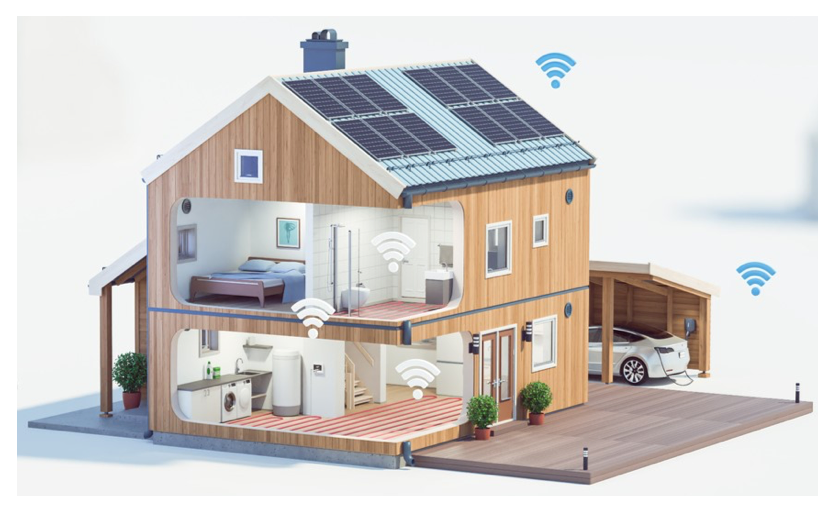
\includegraphics[width=1\textwidth,clip]{Figures/SmartHouse.eps}}

\tikzstyle{Sys_block} = [rectangle, draw, fill=none,  text width=3.cm, text centered, rounded corners, minimum height=4em,inner sep=2pt]
\tikzstyle{Obj_block} = [rectangle, draw, fill=myLightRed,  text width=2.7cm, text centered, rounded corners, minimum height=4em,inner sep=2pt]
\tikzstyle{Opt_block} = [rectangle, draw, fill=myLightGreen,  text width=3cm,  text centered, rounded corners]
\tikzstyle{ID_block} = [rectangle, draw, fill=myLightBlue,  text width=3cm, text centered, rounded corners]    
\tikzstyle{line} = [draw, -latex']

\begin{tikzpicture}[->,>=stealth']

\node [Sys_block] (sys0) {\Sys};

\node [ID_block, left of=sys0, node distance = 5cm] (ID0) {
 \begin{minipage}[c]{3cm}
\textbf{AI model} e.g.
\begin{align*}
\hat{\vect{s}}_{+} \sim \rho_{\vect{\theta}}\left(\cdot\,|\,\vect{s},\vect{a}\right)
\end{align*}
\vspace{-.75cm}
\flushright fitting data $\rho$
\end{minipage}
 };


 
 \node [Opt_block, below of=ID0, node distance = 2.7cm] (opt0) {
 \begin{minipage}[c]{3cm}
 \center
\textbf{Policy}\\
 \vspace{-0.6cm}
\begin{align*}
\vect\pi_{\vect\theta}(\vect{s})
\end{align*}
 \vspace{-0.5cm}\\
optimal for AI model 
\end{minipage}
 };
 
 \node [Obj_block, left of=opt0, node distance = 4cm] (Obj0) {
 \begin{minipage}[c]{2.7cm}
\textbf{Objective}
\vspace{-.5cm}\\
\begin{align*}
L\left(\vect s,\vect a\right)
\end{align*}
\vspace{-1.25cm}\\
\flushright possibly unbounded
\end{minipage}
 };
 
 \path 
 (sys0) edge  node[anchor=center,xshift=-.5em] {
  \begin{minipage}[c]{1cm}
  \center
 Data\\ knowledge
 \end{minipage}} (ID0)
 (ID0) edge[bend left=20]  node[anchor=west] {Predictions} (opt0)
 (opt0) edge[bend left=20]  node[anchor=east] {Actions} (ID0)
 (opt0) edge[bend right=20]  node[anchor=west,xshift=1em] {Policy} (sys0)
 (Obj0) edge  node[anchor=south] {Cost} (opt0)
 ;
\end{tikzpicture}

\textbf{Learning model $\rho_{\vect{\theta}}$ should aim at identifying 
}
\begin{align}
\label{eq:Jmin}
\vect{\theta}^\star =\argmin_{\vect{\theta} }\,J\left(\vect\pi_{\vect{\theta} }\right)
\end{align}
\vspace{-.6cm}
\visible<2->{
\begin{itemize}
\item Closed-loop performance $J$ is intricate ($\vect\theta\,\rightarrow\,$simulations$\,\rightarrow\,$policy$\,\rightarrow\,$real system)
\item \visible<3->{$\nabla_{\vect\theta}J\left(\vect\pi_{\vect\theta}\right)$ is to be estimated from data, i.e. data hungry, noisy, possible biases}
\item \visible<4->{\eqref{eq:Jmin} is in general different than model fitting, i.e. no loss function does  \eqref{eq:Jmin}}
\end{itemize}
}


\end{frame}




\begin{frame}{\normalsize Optimal AI models for Decision - A Paradigm Shift}
\footnotesize

\newcommand{\Sys}{\vspace{-0.25cm}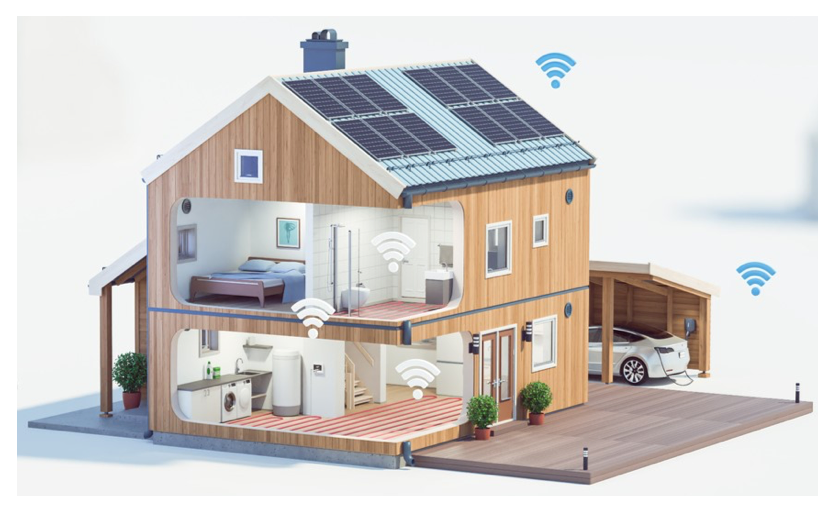
\includegraphics[width=1\textwidth,clip]{Figures/SmartHouse.eps}}

\tikzstyle{Sys_block} = [rectangle, draw, fill=none,  text width=3.cm, text centered, rounded corners, minimum height=4em,inner sep=2pt]
\tikzstyle{Obj_block} = [rectangle, draw, fill=myLightRed,  text width=2.7cm, text centered, rounded corners, minimum height=4em,inner sep=2pt]
\tikzstyle{Opt_block} = [rectangle, draw, fill=myLightGreen,  text width=3cm,  text centered, rounded corners]
\tikzstyle{ID_block} = [rectangle, draw, fill=myLightBlue,  text width=3cm, text centered, rounded corners]    
\tikzstyle{line} = [draw, -latex']

\begin{tikzpicture}[->,>=stealth']

\node [Sys_block] (sys0) {\Sys};

\node [ID_block, left of=sys0, node distance = 5cm] (ID0) {
 \begin{minipage}[c]{3cm}
\textbf{AI model} 
\begin{align*}
\hat{\vect{s}}_{+} \sim \rho_{\vect{\theta}}\left(\cdot\,|\,\vect{s},\vect{a}\right)
\end{align*}
\vspace{-.75cm}
 \visible<1-3>{\flushright fitting data $\rho$}
\end{minipage}
 };


 
 \node [Opt_block, below of=ID0, node distance = 3cm] (opt0) {
 \begin{minipage}[c]{3cm}
 \center
\textbf{Policy}
 \vspace{-0.1cm}
\begin{align*}
\vect\pi_{\vect \theta}(\vect{s})
\end{align*}
optimal for AI model
\end{minipage}
 };
 
 \node [Obj_block, left of=opt0, node distance = 4cm] (Obj0) {
 \begin{minipage}[c]{2.7cm}
\textbf{Objective}
\vspace{-.5cm}\\
\begin{overlayarea}{\textwidth}{0.1\textheight}
\only<1-2>{
\begin{align*}
L\left(\vect s,\vect a\right)
\end{align*}
}
\only<3->{
\begin{align*}
L_{\vect\theta}\left(\vect s,\vect a\right)
\end{align*}
}
\end{overlayarea}
\flushright possibly unbounded
\end{minipage}
 };
 
 \path 
 (sys0) edge  node[anchor=center,xshift=-.5em] {
  \begin{minipage}[c]{1cm}
  \center
 Data\\ knowledge
 \end{minipage}} (ID0)
 (ID0) edge[bend left=20]  node[anchor=west] {Predictions} (opt0)
 (opt0) edge[bend left=20]  node[anchor=east] {Actions} (ID0)
 (opt0) edge[bend right=20]  node[anchor=west,xshift=1em] {Policy} (sys0)
 (Obj0) edge  node[anchor=south] {Cost} (opt0)
 ;
 

 \visible<2->{\draw[blue,thick] ($(ID0.north east)+(+0.15,0.15)$)  rectangle ($(Obj0.south west)+(-0.15,-0.3)$);}
 
 
\end{tikzpicture}


\begin{overlayarea}{\textwidth}{0.25\textheight}



\only<2-4>{
\begin{itemize}
\item  The model is not $ \rho_{\vect{\theta}}$, it is the entire \textcolor{blue}{``decision-making box"}
\item  \visible<3->{The model includes objective $L_{\vect \theta}$ used to build the policy$^\star$}
\item  \visible<4->{Best model $\rho_{\vect\theta}$ should \textit{not necessarily} represent the data in a ``classical sense"}
\end{itemize}
\vspace{.5cm}
\visible<3->{\scriptsize $^\star$ policy performance on real system still assessed via $L$}
}

\only<5->{
\begin{alertblock}{}
\center
\textbf{Theorem}: under some (technical) assumptions, there is a $L_{\vect \theta}$ such that $\vect\pi_{\vect \theta}=\vect\pi_\star$, even if $ \rho_{\vect{\theta}}$ does not represent real world $\rho$ correctly
\end{alertblock}
}

\end{overlayarea}


\end{frame}







\begin{frame}{\normalsize How to use this more generally? RL over Policy Training}
\footnotesize

\newcommand{\Sys}{\vspace{-0.25cm}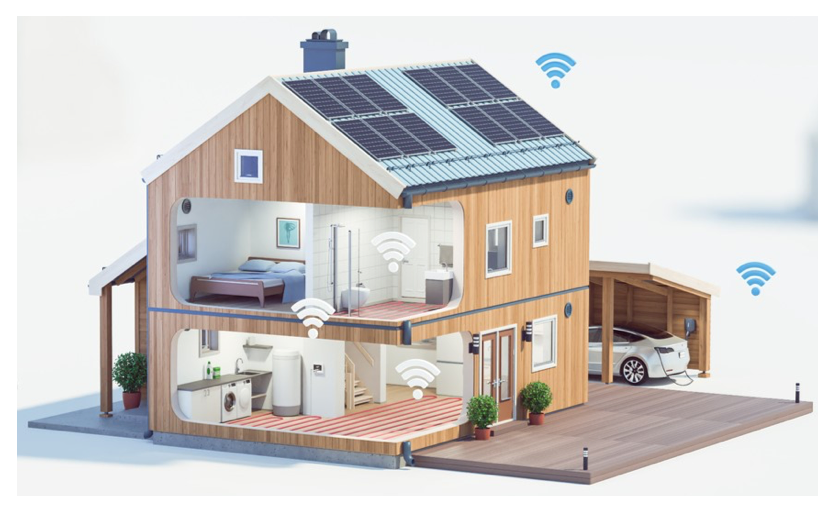
\includegraphics[width=1\textwidth,clip]{Figures/SmartHouse.eps}}

\tikzstyle{Sys_block} = [rectangle, draw, fill=none,  text width=3.cm, text centered, rounded corners, minimum height=4em,inner sep=2pt]
\tikzstyle{Obj_block} = [rectangle, draw, fill=myLightRed,  text width=2.7cm, text centered, rounded corners, minimum height=4em,inner sep=2pt]
\tikzstyle{Opt_block} = [rectangle, draw, fill=myLightGreen,  text width=3cm,  text centered, rounded corners]
\tikzstyle{ID_block} = [rectangle, draw, fill=myLightBlue,  text width=3cm, text centered, rounded corners]    

\tikzstyle{RL_block} = [rectangle, draw, fill=none,  text width=3.cm, text centered, rounded corners, minimum height=4em,inner sep=2pt]

\tikzstyle{line} = [draw, -latex']

\begin{tikzpicture}[->,>=stealth']

\node [Sys_block] (sys0) {\Sys};

\node [ID_block, left of=sys0, node distance = 5cm] (ID0) {
 \begin{minipage}[c]{3cm}
\textbf{AI model} 
 \vspace{-0.2cm}
\begin{align*}
\hat{\vect{s}}_{+} \sim \rho_{\vect{\theta}}\left(\cdot\,|\,\vect{s},\vect{a}\right)
\end{align*}
%\vspace{-.75cm}
% \visible<1-4>{\flushright fitting data}
\end{minipage}
 };

\visible<2->{
\node [RL_block, above of=ID0, node distance = 2cm] (RL0) {
 \begin{minipage}[c]{3cm}
\textbf{RL} 
\vspace{-.1cm} 
\begin{align*}
\Delta\vect\theta = \alpha\nabla_{\vect\theta} J\left(\vect\pi_{\vect \theta}\right)
\end{align*}
\vspace{-.85cm}
\flushright from data
\end{minipage}
 };}

 
 \node [Opt_block, below of=ID0, node distance = 2.0cm] (opt0) {
 \begin{minipage}[c]{3cm}
 \center
\textbf{Policy}
 \vspace{-0.2cm}
\begin{align*}
\vect\pi_{\vect \theta}(\vect{s})
\end{align*}
% \vspace{-0.25cm}\\
optimal for AI model
\end{minipage}
 };
 
 \node [Obj_block, left of=opt0, node distance = 4cm] (Obj0) {
 \begin{minipage}[c]{2.7cm}
\textbf{In-Sim Objective}
\vspace{-.5cm}\\
\begin{align*}
L_{\vect \theta}\left(\vect s,\vect a\right)
\end{align*}
\end{minipage}
 };
 
  \visible<2->{
  \node [Obj_block, left of=RL0, node distance = 4cm] (Obj1) {
 \begin{minipage}[c]{2.7cm}
\textbf{In-Real Objective}
\vspace{-.5cm}\\
\begin{align*}
L\left(\vect s,\vect a\right)
\end{align*}
\end{minipage}
 };}
 
 \path 
 (sys0) edge  node[anchor=center,xshift=-.5em] {
  \begin{minipage}[c]{1cm}
  \center
 Data\\ knowledge
 \end{minipage}} (ID0)
 (ID0) edge[bend left=20]  node[anchor=west] {Predictions} (opt0)
 (opt0) edge[bend left=20]  node[anchor=east] {Actions} (ID0)
 (opt0) edge[bend right=20]  node[anchor=west,xshift=1em] {Policy} (sys0)
 (Obj0) edge  node[anchor=south] {Cost} (opt0)
 ;
 
 \visible<2->{
 \path   (sys0) edge[bend right=20]  node[anchor=south west] {
  \begin{minipage}[c]{1cm}
  \center
 Data\\ knowledge
 \end{minipage}} (RL0)
   (RL0) edge[bend right=20]  node[anchor=south east] {$\Delta\vect\theta$} (Obj0)
  (RL0) edge  node[anchor=west] {$\Delta\vect\theta$} (ID0)
   (Obj1) edge  node[anchor=south east] {} (RL0)
  ;}


\draw[blue,thick] ($(ID0.north east)+(+0.15,0.15)$)  rectangle ($(Obj0.south west)+(-0.15,-0.3)$);
 
 
\end{tikzpicture}
\vspace{.2cm}
\begin{overlayarea}{\textwidth}{0.25\textheight}
\only<3>{\textbf{Policy gradient}
$$\nabla_{\vect \theta}J(\vect\pi_{\vect\theta}) = \mathbb E\left[ \nabla_{\vect \theta}\vect\pi_{\vect\theta} \nabla_{\vect a} Q^{\vect\pi_{\vect\theta}}\right]$$
\vspace{-.5cm}
\begin{itemize}
\item $Q^{\vect\pi_{\vect\theta}}$ is the critic, well-established RL tool
\item $\nabla_{\vect \theta}\vect\pi_{\vect\theta}$ requires differentiating the closed-loop simulation...
\end{itemize}
}
\only<4->{
\begin{block}{}
\center
\textbf{Difficulty}: computing $\nabla_{\vect \theta}\vect\pi_{\vect\theta}$ requires total differentiation through the simulation-based policy optimization process: \\
\textcolor{myBlue2}{$\vect\theta\,\rightarrow\,$simulations\textcolor{myRed2}{$\,\rightarrow\,$}optimal policy for $\rho_{\vect\theta}$}\\
Differentiating through policy optimization can be \textcolor{myRed2}{computationally heavy}
%\begin{itemize}
%\item ...
%\end{itemize}
%\textbf{Ingredients:}
%\begin{itemize}
%\item $Q^{\vect\pi_{\vect\theta}}$ is the ``critic", well-established RL methods to compute it
%\item $\nabla_{\vect \theta}\vect\pi_{\vect\theta}$ requires differentiating the optimal planning at every time step. Efficient methods are now available.
%\end{itemize}
\end{block}
}
\end{overlayarea}
\end{frame}

%%%%%%%%%%%%%%%%%%%%%%%%%%%%%%%%%%%%%%%%%%%%%%%%%%%%%%%%%%%%%%%%%%%%%%%%
%%%%%%%%%%%%%%%%%%%%%%%%%%%%%%%%%%%%%%%%%%%%%%%%%%%%%%%%%%%%%%%%%%%%%%%%
%  NEW PART: differentiating policy training w.r.t. MDP parameters
%  Colour code: red theta = MDP (simulator / cost / design) parameters,
%               blue nu   = policy parameters,
%               orange LR = likelihood-ratio, green PD = pathwise.
%%%%%%%%%%%%%%%%%%%%%%%%%%%%%%%%%%%%%%%%%%%%%%%%%%%%%%%%%%%%%%%%%%%%%%%%
%%%%%%%%%%%%%%%%%%%%%%%%%%%%%%%%%%%%%%%%%%%%%%%%%%%%%%%%%%%%%%%%%%%%%%%%

\section{Differentiating Policy Training}

%-----------------------------------------------------------------------
\begin{frame}{\normalsize What we need: the sensitivity of a trained policy}
\footnotesize
\tikzstyle{ID_block} = [rectangle, draw, fill=myLightBlue, text centered, rounded corners, minimum height=3.3em, inner sep=3pt]
\tikzstyle{Opt_block} = [rectangle, draw, fill=myLightGreen, text centered, rounded corners, minimum height=3.3em, inner sep=3pt]
\begin{center}
\begin{tikzpicture}[->,>=stealth', node distance=0.6cm]
\node (th) {$\mth$};
\node[ID_block, right=of th] (sim) {\begin{minipage}{1.9cm}\centering\textbf{Simulator}\\[2pt] $\rth,\ \Lth$\end{minipage}};
\node[Opt_block, right=of sim] (rl) {\begin{minipage}{2.8cm}\centering\textbf{In-sim RL}\\[2pt] many noisy updates of $\pnu$\end{minipage}};
\node[right=of rl] (nu) {$\nst(\mth)$};
\draw (th) -- (sim); \draw (sim) -- (rl); \draw (rl) -- (nu);
\end{tikzpicture}
\end{center}
\vspace{-.3cm}
\begin{columns}[T]
\column{0.47\textwidth}
\textbf{In-sim policy training}, for a given $\mth$
\begin{align*}
\nst(\mth) &= \argmin_{\pnu}\ \Jh(\pnu)\\
\Jh(\pnu) &= \E_{\rth,\,\pin}\Big[\sum\nolimits_{k}\gamma^k \Lth(\sv_k,\av_k)\Big]
\end{align*}
\column{0.51\textwidth}
\visible<2->{
\textbf{Policy sensitivity}
\begin{align*}
\kap := \frac{\mathrm d\nst}{\mathrm d\mth}\in\mathbb R^{\dim\pnu\times\dim\mth}
\end{align*}

\vspace{-.15cm}
{\scriptsize This is the missing piece of the previous slide: \ $\nabla_{\vect\theta}\vect\pi_{\vect\theta}=\nabla_{\pnu}\pin\big|_{\nst}\,\kap$}}
\end{columns}
\vspace{.1cm}
\visible<3->{
\textbf{How to get} $\kap$\textbf{?}
\begin{enumerate}
\scriptsize
\item \textbf{Unroll training}: backpropagate through all updates $\pnu_{j+1}=\pnu_j-\beta\,\hat g_j$\\
\textcolor{myRed2}{\ding{56}} cost $\propto$ number of updates
\item \visible<4->{\textbf{Differentiate the Bellman optimality equations} (Nikishin et al., 2022)\\
\textcolor{myRed2}{\ding{56}} needs $\pi=$ softmax$(Q^\star)$}
\item \visible<5->{\textbf{Implicitly differentiate the \emph{end point} of training}\\
\textcolor{myGreen3}{\ding{52}} any policy class, any policy gradient}
\end{enumerate}}
\visible<6->{
\begin{alertblock}{}
\center So first: How do we differentiate through an MDP at all?
\end{alertblock}}
\end{frame}

%-----------------------------------------------------------------------
\begin{frame}{\normalsize Two ways to differentiate an expectation}
\footnotesize
\begin{itemize}
\item \textbf{Problem}: estimate $\nabla_{\psi}\,\E_{x\sim p_{\psi}}\big[f(x)\big]$ from samples $x_1,\dots,x_n\sim p_\psi$ \ {\scriptsize($\psi$: later $\mth$ or $\pnu$)}
\item<2-> \textbf{Idea}: a gradient is the change of the sample average when $\psi$ moves a little\\[2pt]
\hspace*{1cm}$\displaystyle\nabla_\psi\E\big[f(x)\big]\approx\frac{\E_{\psi+\mathrm d\psi}[f]-\E_{\psi}[f]}{\mathrm d\psi},\qquad \E_{\psi}[f]\approx\frac1n\sum\nolimits_i f(x_i)$
\item<2-> \textbf{Question}: how to get the \emph{new} average $\E_{\psi+\mathrm d\psi}[f]$ from the \emph{same} samples?
\end{itemize}
\vspace{-.2cm}
\begin{columns}[T,onlytextwidth]
\column{0.485\textwidth}
\visible<3->{
\begin{block}{\footnotesize \LR\ (likelihood ratio): \textbf{re-weight} samples}
\vspace{-.3cm}
\begin{align*}
\nabla_\psi \E\big[f(x)\big] = \E\Big[f(x)\,\textcolor{myOrangeD}{\nabla_\psi\log p_\psi(x)}\Big]
\end{align*}

\vspace{-.35cm}
\begin{center}
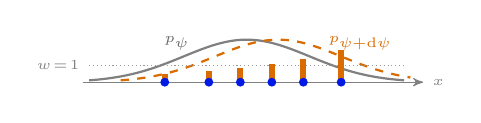
\begin{tikzpicture}[x=0.8cm, y=0.72cm, >=stealth']
\draw[->, black!50] (-2.6,0) -- (2.8,0) node[right, font=\tiny]{$x$};
\draw[black!50, thick] plot[domain=-2.5:2.5, samples=60, smooth] (\x,{0.75*exp(-\x*\x/2)});
\node[font=\tiny, text=black!60, anchor=east] at (-0.75,0.68) {$p_\psi$};
\draw[myOrangeD, thick, dashed, visible on=<5->] plot[domain=-2.0:2.6, samples=60, smooth] (\x,{0.75*exp(-(\x-0.5)*(\x-0.5)/2)});
\node[font=\tiny, text=myOrangeD, anchor=west, visible on=<5->] at (1.15,0.68) {$p_{\psi+\mathrm d\psi}$};
\draw[black!40, densely dotted, visible on=<4->] (-2.5,0.3) -- (2.5,0.3);
\node[font=\tiny, text=black!50, anchor=east, visible on=<4->] at (-2.5,0.3) {$w\!=\!1$};
\foreach \x/\w in {-1.3/0.46, -0.6/0.65, -0.1/0.84, 0.4/1.08, 0.9/1.38, 1.5/1.87}{
  \draw[myOrangeD, line width=2.2pt, visible on=<4->] (\x,0) -- (\x,{0.3*\w});
  \fill[myBlue3] (\x,0) circle (1.6pt);
}
\end{tikzpicture}
\end{center}
\vspace{-.25cm}
\scriptsize
\setlength{\leftmargini}{1.4em}
\begin{itemize}
\setlength{\itemsep}{3pt}
\item samples $x_i\sim p_\psi$ stay where they are
\item<4-> $w_i=\frac{p_{\psi+\mathrm d\psi}}{p_\psi}(x_i)\approx1+\textcolor{myOrangeD}{\nabla_\psi\log p_\psi(x_i)}\,\mathrm d\psi$
\item<5-> new average $\approx\frac1n\sum_i w_i\,f(x_i)$
\end{itemize}
\end{block}}
\column{0.485\textwidth}
\visible<6->{
\begin{block}{\footnotesize \PD\ (reparameterization): \textbf{move} samples}
\vspace{-.3cm}
\begin{align*}
\nabla_\psi \E\big[f(x)\big] = \E_{\varepsilon}\Big[\textcolor{myGreen3}{\nabla_x f(x)\,\nabla_\psi g_\psi(\varepsilon)}\Big]
\end{align*}

\vspace{-.35cm}
\begin{center}
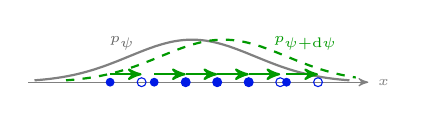
\begin{tikzpicture}[x=0.8cm, y=0.72cm, >=stealth']
\draw[->, black!50] (-2.6,0) -- (2.8,0) node[right, font=\tiny]{$x$};
\draw[black!50, thick] plot[domain=-2.5:2.5, samples=60, smooth] (\x,{0.75*exp(-\x*\x/2)});
\node[font=\tiny, text=black!60, anchor=east] at (-0.75,0.68) {$p_\psi$};
\draw[myGreen3, thick, dashed, visible on=<8->] plot[domain=-2.0:2.6, samples=60, smooth] (\x,{0.75*exp(-(\x-0.5)*(\x-0.5)/2)});
\node[font=\tiny, text=myGreen3, anchor=west, visible on=<8->] at (1.15,0.68) {$p_{\psi+\mathrm d\psi}$};
\foreach \x in {-1.3, -0.6, -0.1, 0.4, 0.9, 1.5}{
  \draw[->, myGreen3, thick, visible on=<7->] (\x,0.14) -- ({\x+0.5},0.14);
  \fill[myBlue3] (\x,0) circle (1.6pt);
  \draw[myBlue3, visible on=<7->] ({\x+0.5},0) circle (1.6pt);
}
\end{tikzpicture}
\end{center}
\vspace{-.25cm}
\scriptsize
\setlength{\leftmargini}{1.4em}
\begin{itemize}
\setlength{\itemsep}{3pt}
\item samples $x_i=g_\psi(\varepsilon_i)$, \ noise $\varepsilon_i\sim p(\varepsilon)$
\item<7-> keep $\varepsilon_i$, move: $x_i'\approx x_i+\textcolor{myGreen3}{\nabla_\psi g_\psi(\varepsilon_i)}\,\mathrm d\psi$
\item<8-> new average $\approx\frac1n\sum_i f(x_i')$
\end{itemize}
\end{block}}
\end{columns}
\visible<3->{\vspace{.1cm}\centering
{\scriptsize Pictures: $\psi=\mu$, \ $x=\mu+\varepsilon$, \ $\varepsilon\sim\mathcal N(0,1)$; \ gray $=p_\psi$, \ dashed $=p_{\psi+\mathrm d\psi}$}\par}
\end{frame}

%-----------------------------------------------------------------------
\begin{frame}{\normalsize Two families of policy gradients}
\footnotesize
\textbf{RL}: \ $x\to$ trajectory $\tau=(\sv_0,\av_0,\sv_1,\dots)$, \ $\psi\to\pnu$, \ $f\to\sum_k\gamma^k\Lth(\sv_k,\av_k)$\\[3pt]
\begin{columns}[T,onlytextwidth]
\column{0.485\textwidth}
\visible<2->{
\begin{block}{\footnotesize \LR\ (score function): \textbf{re-weight} trajectories}
\scriptsize
\setlength{\leftmargini}{1.4em}\setlength{\leftmarginii}{1.4em}
\setbeamerfont{itemize/enumerate subbody}{size=\scriptsize}
\begin{itemize}
\setlength{\itemsep}{3pt}
\item $\tau$ has a \textbf{density}:\\ $p(\tau)=\rho_0(\sv_0)\prod_k\pin(\av_k|\sv_k)\,\rth(\sv_{k+1}|\sv_k,\av_k)$
\item<3-> score: $\nabla_{\pnu}\log p(\tau)=\sum_k\textcolor{myOrangeD}{\nabla_{\pnu}\log\pin(\av_k|\sv_k)}$
\begin{itemize}
\item<4-> the model $\rth$ drops out
\end{itemize}
\end{itemize}
\end{block}}
\column{0.485\textwidth}
\visible<5->{
\begin{block}{\footnotesize \PD\ (pathwise): \textbf{move} trajectories}
\scriptsize
\setlength{\leftmargini}{1.4em}\setlength{\leftmarginii}{1.4em}
\setbeamerfont{itemize/enumerate subbody}{size=\scriptsize}
\begin{itemize}
\setlength{\itemsep}{3pt}
\item $\tau$ is a \textbf{function} of fixed noise $(\varepsilon_k,\xi_k)$:\\ $\av_k=g_{\pnu}(\sv_k,\varepsilon_k)$, \ $\sv_{k+1}=f_{\mth}(\sv_k,\av_k,\xi_k)$
\item<6-> gradients: $\textcolor{myGreen3}{\tfrac{\mathrm d\sv_{k+1}}{\mathrm d\pnu}}=\nabla_{\sv}f_{\mth}\tfrac{\mathrm d\sv_{k}}{\mathrm d\pnu}+\nabla_{\av}f_{\mth}\tfrac{\mathrm d\av_{k}}{\mathrm d\pnu}$
\begin{itemize}
\item<7-> the model $f_{\mth}$ stays in
\end{itemize}
\end{itemize}
\end{block}}
\end{columns}
\vspace{.05cm}
\visible<8->{\textbf{The policy gradient in the two views}}
\begin{alignat*}{2}
\visible<8->{\LR:\quad\nabla_{\pnu}\Jh}&\visible<8->{=\E\Big[\sum\nolimits_k\gamma^k\,\textcolor{myOrangeD}{\nabla_{\pnu}\log\pin(\av_k|\sv_k)}\,Q^{\pin}_{\mth}(\sv_k,\av_k)\Big]}
&&\quad\visible<8->{\text{\scriptsize REINFORCE, A2C, PPO}}\\
\visible<9->{\PD:\quad\nabla_{\pnu}\Jh}&\visible<9->{=\E_\omega\Big[\sum\nolimits_k\gamma^k\big(\nabla_{\sv}\Lth\,\textcolor{myGreen3}{\tfrac{\mathrm d\sv_k}{\mathrm d\pnu}}+\nabla_{\av}\Lth\,\textcolor{myGreen3}{\tfrac{\mathrm d\av_k}{\mathrm d\pnu}}\big)\Big]}
&&\quad\visible<9->{\text{\scriptsize BPTT, SVG, SAC (SVG(0))}}
\end{alignat*}
\visible<10->{
\begin{alertblock}{}
\textbf{Two estimates of the same gradient, but the simulator $\mth$ sits in different places}:\\
\LR: only in the \textbf{sampling} ($\rth$) and the critic $Q_{\mth}$; \quad \PD: inside each path, through the \textbf{Jacobians} of $f_{\mth}$.\\
{\scriptsize This decides how we will differentiate training with respect to $\mth$ later.}
\end{alertblock}}
\end{frame}

%-----------------------------------------------------------------------
\begin{frame}{\normalsize LR or PD? Requirements, bias and variance}
\footnotesize
\begin{center}
\renewcommand{\arraystretch}{1.45}
\setlength{\tabcolsep}{6pt}
\begin{tabular}{l|l|l}
 & \LR\ (re-weight) & \PD\ (move)\\ \hline
needs & samples and $\nabla_{\pnu}\log\pin$ & derivatives of $f_{\mth}$, $g_{\pnu}$, $\Lth$\\
\uncover<2->{simulator} & \uncover<2->{black box is fine} & \uncover<2->{must be differentiable}\\
\uncover<3->{bias} & \uncover<3->{none} & \uncover<3->{at jumps (contacts, $\min$/$\max$)}\\
\uncover<4->{variance grows with} & \uncover<4->{size of $Q$, horizon} & \uncover<4->{products of Jacobians $\nabla f_{\mth}$}\\
\uncover<5->{reduce variance} & \uncover<5->{baseline, critic: $Q-V$} & \uncover<5->{short horizon $+$ critic (SVG, SHAC)}\\
\end{tabular}
\end{center}
\vspace{-.1cm}
\begin{columns}[c,onlytextwidth]
\column{0.5\textwidth}
\centering
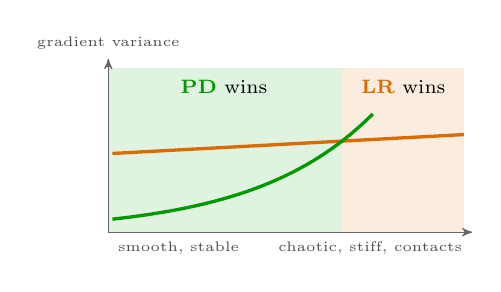
\begin{tikzpicture}[x=1.05cm, y=0.8cm, >=stealth', visible on=<6->]
\fill[myGreen3!12, visible on=<7->] (0,0) rectangle (2.83,2.6);
\fill[myOrangeD!12, visible on=<7->] (2.83,0) rectangle (4.3,2.6);
\node[font=\scriptsize, visible on=<7->] at (1.4,2.3) {\PD\ wins};
\node[font=\scriptsize, visible on=<7->] at (3.57,2.3) {\LR\ wins};
\draw[->, black!60] (0,0) -- (4.4,0);
\draw[->, black!60] (0,0) -- (0,2.75) node[above, font=\tiny, text=black!70]{gradient variance};
\draw[myOrangeD, very thick] (0.05,1.25) -- (4.3,1.55);
\draw[myGreen3, very thick, domain=0.05:3.2, samples=40] plot (\x,{0.2*exp(0.7*\x)});
\node[font=\tiny, text=black!70, anchor=north west] at (0,0) {smooth, stable};
\node[font=\tiny, text=black!70, anchor=north east] at (4.4,0) {chaotic, stiff, contacts};
\end{tikzpicture}
\column{0.47\textwidth}
\visible<7->{
\begin{alertblock}{}
\textbf{Neither always has lower variance.}\\[3pt]
\PD\ is far less noisy on smooth, stable systems, but can be far noisier than \LR\ on chaotic, stiff or contact-rich ones.\\[2pt]
{\scriptsize (Parmas et al., 2018; Suh et al., 2022)}
\end{alertblock}}
\end{columns}
\end{frame}

%-----------------------------------------------------------------------
\begin{frame}{\normalsize The Bellman computational tree}
\footnotesize
\begin{columns}[T]
\column{0.58\textwidth}
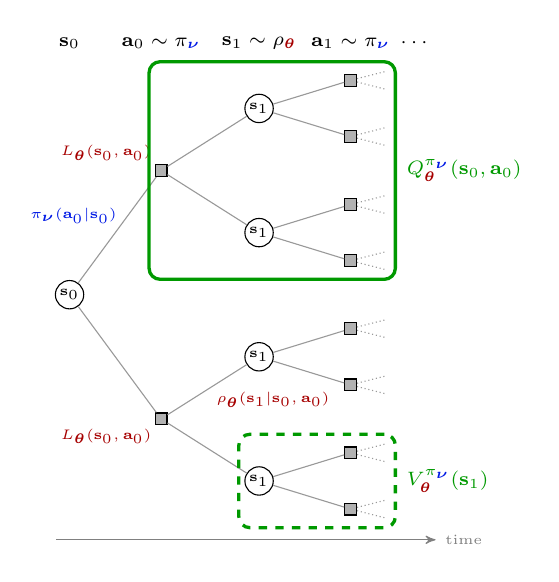
\begin{tikzpicture}[scale=0.83, >=stealth',
  st/.style={circle, draw, fill=white, inner sep=0pt, minimum size=0.36cm, font=\tiny},
  ac/.style={rectangle, draw, fill=black!30, inner sep=0pt, minimum size=0.15cm},
  pe/.style={draw=black!40, onslide=<2->{draw=myBlue3, thick}},
  me/.style={draw=black!40, onslide=<3->{draw=myRed2, thick}}]
% column headers
\foreach \x/\t in {0/{$\sv_0$}, 1.4/{$\av_0\sim\pin$}, 2.9/{$\sv_1\sim\rth$}, 4.3/{$\av_1\sim\pin$}, 5.3/{$\cdots$}}
  \node[font=\scriptsize] at (\x,3.85) {\t};
\draw[->, black!50] (-0.2,-3.75) -- (5.6,-3.75) node[right, font=\tiny]{time};
% tree
\node[st] (r) at (0,0) {$\sv_0$};
\foreach \i/\y in {1/1.9,2/-1.9}{
  \node[ac] (a\i) at (1.4,\y) {};
  \draw[pe] (r) -- (a\i);
  \foreach \j/\dy in {1/0.95,2/-0.95}{
    \node[st] (s\i\j) at (2.9,{\y+\dy}) {$\sv_1$};
    \draw[me] (a\i) -- (s\i\j);
    \foreach \k/\ddy in {1/0.43,2/-0.43}{
      \node[ac] (a\i\j\k) at (4.3,{\y+\dy+\ddy}) {};
      \draw[pe] (s\i\j) -- (a\i\j\k);
      \draw[me, densely dotted] (a\i\j\k) -- ++(0.55,0.14);
      \draw[me, densely dotted] (a\i\j\k) -- ++(0.55,-0.14);
    }
  }
}
% edge labels
\node[visible on=<2->, font=\tiny, text=myBlue3, anchor=south east, inner sep=1pt] at ($(r)!0.55!(a1)$) {$\pin(\av_0|\sv_0)$};
\node[visible on=<3->, font=\tiny, text=myRed2, anchor=north west, inner sep=1pt] at ($(a2)!0.5!(s21)+(0.05,-0.02)$) {$\rth(\sv_1|\sv_0,\av_0)$};
% costs at action nodes
\node[visible on=<3->, font=\tiny, text=myRed2, anchor=south east, inner sep=1pt] at (a1.north west) {$\Lth(\sv_0,\av_0)$};
\node[visible on=<3->, font=\tiny, text=myRed2, anchor=north east, inner sep=1pt] at (a2.south west) {$\Lth(\sv_0,\av_0)$};
% subtrees (values)
\coordinate (t1) at ($(a111)+(0.6,0.2)$);
\coordinate (t2) at ($(a122)+(0.6,-0.2)$);
\node[visible on=<4->, draw=myGreen3, very thick, rounded corners, fit=(a1)(a111)(a122)(t1)(t2), inner sep=2pt] (subQ) {};
\node[visible on=<4->, text=myGreen3, font=\scriptsize, anchor=west] at (subQ.east) {$Q^{\pin}_{\mth}(\sv_0,\av_0)$};
\coordinate (t3) at ($(a221)+(0.6,0.2)$);
\coordinate (t4) at ($(a222)+(0.6,-0.2)$);
\node[visible on=<4->, draw=myGreen3, very thick, dashed, rounded corners, fit=(s22)(a221)(a222)(t3)(t4), inner sep=2pt] (subV) {};
\node[visible on=<4->, text=myGreen3, font=\scriptsize, anchor=west] at (subV.east) {$V^{\pin}_{\mth}(\sv_1)$};
\end{tikzpicture}
\column{0.4\textwidth}
\textbf{All possible histories}: every root-to-leaf path is one trajectory; its probability is the product of its edge probabilities
\begin{align*}
\Jh(\pnu) = \sum_{\text{paths}}P(\text{path})\sum_k\gamma^k\Lth
\end{align*}

\vspace{-.3cm}
\visible<2->{\begin{itemize}
\item \textcolor{myBlue3}{\textbf{Policy edges}} $\pin(\av|\sv)$: \\$\pnu$ lives here
\item \visible<3->{\textcolor{myRed2}{\textbf{Model edges}} $\rth(\sv'|\sv,\av)$ and \textcolor{myRed2}{\textbf{costs}} $\Lth(\sv,\av)$ at the action nodes: $\mth$ lives here}
\end{itemize}}
\visible<4->{
\textcolor{myGreen3}{\textbf{Value of a subtree}} (Bellman)
\begin{align*}
Q(\sv,\av)&=\Lth(\sv,\av)+\gamma\,\E_{\sv'\sim\rth}\big[V(\sv')\big]\\
V(\sv)&=\E_{\av\sim\pin}\big[Q(\sv,\av)\big]
\end{align*}}
\end{columns}
\vspace{-.55cm}
\visible<5->{
\begin{alertblock}{}
\scriptsize In the \LR\ policy gradient $\E\big[\sum_k\gamma^k\nabla_{\pnu}\log\pin\,Q\big]$, $\mth$ acts in two places: the \textcolor{myRed2}{\textbf{edges above}} a node (which histories are sampled) and the \textcolor{myGreen3}{\textbf{subtree below}} it ($Q$). \textbf{Differentiating training with respect to $\mth$ means tracking both.}
\end{alertblock}}
\end{frame}

%-----------------------------------------------------------------------
\begin{frame}{\normalsize Stochastic trajectories: sampling the tree}
\footnotesize
\begin{columns}[T]
\column{0.4\textwidth}
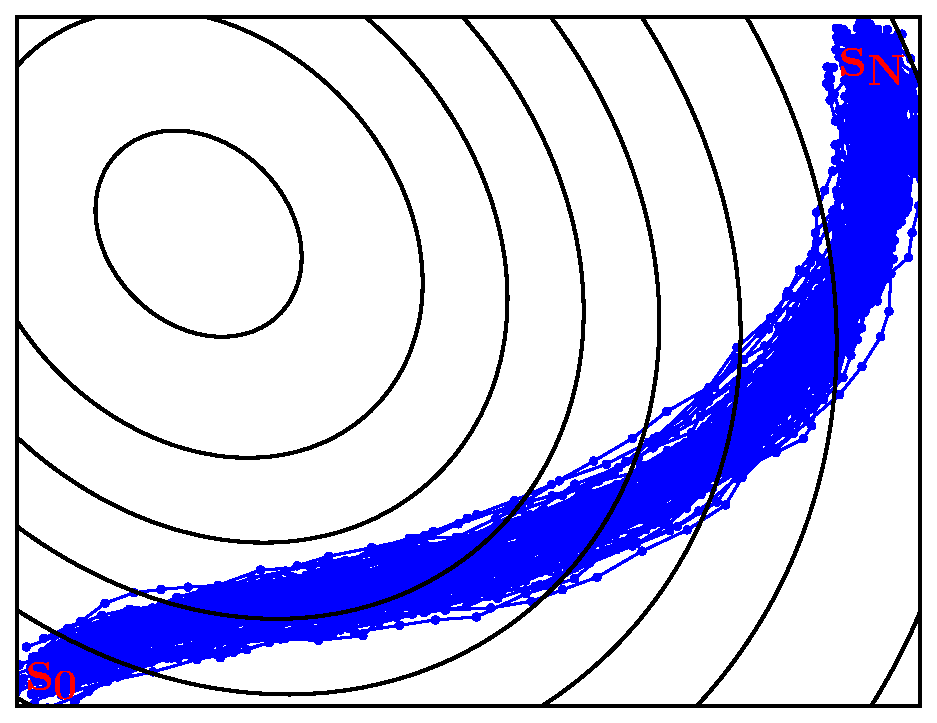
\includegraphics[width=\textwidth]{RLRL/ProbabilisticModel.pdf}\\[2pt]
{\scriptsize The tree has $(|\mathcal A||\mathcal S|)^N$ paths: we never enumerate it, we \textbf{sample} it.\\[2pt]
$n$ simulated closed-loop trajectories from $\sv_0$ to $\sv_N$ = $n$ sampled root-to-leaf paths of the tree}
\begin{align*}
\Jh(\pnu)\approx\frac1n\sum_{i=1}^n\sum_{k=0}^N\gamma^k\Lth(\sv_k^i,\av_k^i)
\end{align*}
\column{0.58\textwidth}
\visible<2->{\textbf{Perturb} $\mth\to\mth+\mathrm d\mth$: what happens to the samples?\\[3pt]
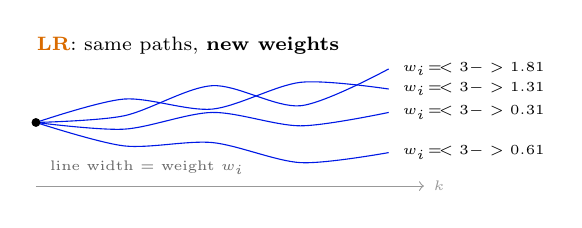
\begin{tikzpicture}[x=1.12cm,y=0.85cm]
\node[anchor=west, font=\scriptsize] at (-0.1,1.15) {\LR: same paths, \textbf{new weights}};
\draw[->, black!40] (0,-0.95) -- (4.4,-0.95) node[right, font=\tiny]{$k$};
% line width = weight: all equal at \mth (overlay 2), re-weighted at \mth+d\mth (overlay 3)
\draw[myBlue3, alt=<3->{line width=2.2pt}{line width=1.2pt}] plot[smooth] coordinates {(0,0)(1,0.1)(2,0.55)(3,0.25)(4,0.8)};
\draw[myBlue3, alt=<3->{line width=1.6pt}{line width=1.2pt}] plot[smooth] coordinates {(0,0)(1,0.35)(2,0.2)(3,0.6)(4,0.5)};
\draw[myBlue3, alt=<3->{line width=0.35pt}{line width=1.2pt}] plot[smooth] coordinates {(0,0)(1,-0.1)(2,0.15)(3,-0.05)(4,0.15)};
\draw[myBlue3, alt=<3->{line width=0.7pt}{line width=1.2pt}] plot[smooth] coordinates {(0,0)(1,-0.35)(2,-0.3)(3,-0.6)(4,-0.45)};
\fill (0,0) circle (1.6pt);
\foreach \y/\w in {0.8/1.8, 0.5/1.3, 0.15/0.3, -0.45/0.6}
  \node[font=\tiny, anchor=west, alt=<3->{text=myOrangeD}{text=black!60}] at (4.05,\y) {$w_i\!=\!\alt<3->{\w}{1}$};
\node[font=\tiny, anchor=south west, text=black!60] at (0.05,-0.93) {line width $=$ weight $w_i$};
\end{tikzpicture}\\
\visible<3->{{\scriptsize $w_i=\dfrac{p_{\mth+\mathrm d\mth}(\tau_i)}{p_{\mth}(\tau_i)}\approx 1+\sum_k\textcolor{myOrangeD}{\nabla_{\mth}\log\rth(\sv^i_{k+1}|\sv^i_k,\av^i_k)}\,\mathrm d\mth$}}}\\[4pt]
\visible<4->{
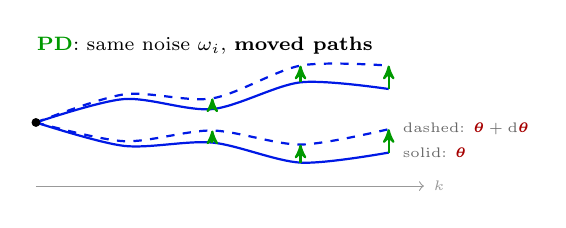
\begin{tikzpicture}[x=1.12cm,y=0.85cm]
\node[anchor=west, font=\scriptsize] at (-0.1,1.15) {\PD: same noise $\omega_i$, \textbf{moved paths}};
\draw[->, black!40] (0,-0.95) -- (4.4,-0.95) node[right, font=\tiny]{$k$};
\draw[myBlue3, thick] plot[smooth] coordinates {(0,0)(1,0.35)(2,0.2)(3,0.6)(4,0.5)};
\draw[myBlue3, thick, dashed, visible on=<5->] plot[smooth] coordinates {(0,0)(1,0.42)(2,0.36)(3,0.85)(4,0.85)};
\draw[myBlue3, thick] plot[smooth] coordinates {(0,0)(1,-0.35)(2,-0.3)(3,-0.6)(4,-0.45)};
\draw[myBlue3, thick, dashed, visible on=<5->] plot[smooth] coordinates {(0,0)(1,-0.28)(2,-0.12)(3,-0.33)(4,-0.1)};
\foreach \x/\a/\b in {2/0.2/0.36, 3/0.6/0.85, 4/0.5/0.85, 2/-0.3/-0.12, 3/-0.6/-0.33, 4/-0.45/-0.1}
  \draw[->, myGreen3, thick, >=stealth', visible on=<5->] (\x,\a) -- (\x,\b);
\fill (0,0) circle (1.6pt);
\node[font=\tiny, anchor=west, text=black!60] at (4.05,-0.45) {solid: $\mth$};
\node[font=\tiny, anchor=west, text=black!60, visible on=<5->] at (4.05,-0.1) {dashed: $\mth+\mathrm d\mth$};
\end{tikzpicture}\\
\visible<5->{{\scriptsize $\sv^i_k(\mth+\mathrm d\mth)\approx\sv^i_k(\mth)+\textcolor{myGreen3}{S^i_k}\,\mathrm d\mth$, \ with \ $\textcolor{myGreen3}{S_k=\mathrm d\sv_k/\mathrm d\mth}$ \ (chain rule along the path)}}}
\end{columns}
\vspace{-.15cm}
\visible<6->{
\begin{alertblock}{}
\center \LR\ changes \textbf{how likely} each history is; \ \PD\ changes \textbf{where} it goes
\end{alertblock}}
\end{frame}

%-----------------------------------------------------------------------
\begin{frame}{\normalsize Differentiating the tree, LR style: edges pass their score down}
\footnotesize
\begin{columns}[T]
\column{0.36\textwidth}
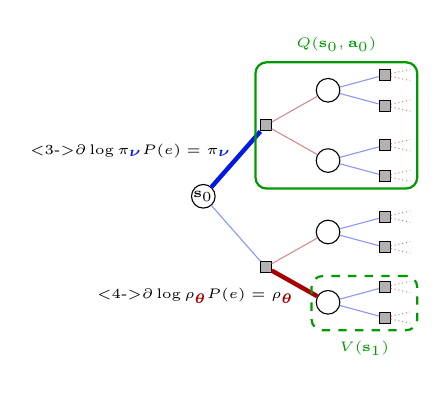
\begin{tikzpicture}[scale=0.72, >=stealth',
  st/.style={circle, draw, fill=white, inner sep=0pt, minimum size=0.3cm, font=\tiny},
  ac/.style={rectangle, draw, fill=black!30, inner sep=0pt, minimum size=0.14cm},
  pe/.style={draw=myBlue3!45},
  me/.style={draw=myRed2!45}]
\node[st] (r) at (0,0) {$\sv_0$};
\foreach \i/\y in {1/1.25,2/-1.25}{
  \node[ac] (a\i) at (1.1,\y) {};
  \draw[pe] (r) -- (a\i);
  \foreach \j/\dy in {1/0.62,2/-0.62}{
    \node[st] (s\i\j) at (2.2,{\y+\dy}) {};
    \draw[me] (a\i) -- (s\i\j);
    \foreach \k/\ddy in {1/0.27,2/-0.27}{
      \node[ac] (a\i\j\k) at (3.2,{\y+\dy+\ddy}) {};
      \draw[pe] (s\i\j) -- (a\i\j\k);
      \draw[me, densely dotted] (a\i\j\k) -- ++(0.45,0.1);
      \draw[me, densely dotted] (a\i\j\k) -- ++(0.45,-0.1);
    }
  }
}
% overlay 2: P(e) on a policy edge and on a model edge; overlay 3: perturb the policy edge
\draw[visible on=<3->, myBlue3, line width=1.6pt] (r) -- (a1);
\node[font=\tiny, visible on=<2->, alt=<3->{text=myOrangeD}{text=myBlue3}, inner sep=1pt, anchor=south east] at ($(r)!0.5!(a1)$) {\alt<3->{$\partial\log\pin$}{$P(e)=\pin$}};
\coordinate (u1) at ($(a111)+(0.5,0.15)$);
\coordinate (u2) at ($(a122)+(0.5,-0.15)$);
\node[visible on=<3->, draw=myGreen3, thick, rounded corners, fit=(a1)(a111)(a122)(u1)(u2), inner sep=1.5pt] (sq) {};
\node[visible on=<3->, font=\tiny, text=myGreen3, anchor=south] at (sq.north) {$Q(\sv_0,\av_0)$};
% overlay 4: perturb the model edge
\draw[visible on=<4->, myRed2, line width=1.6pt] (a2) -- (s22);
\node[font=\tiny, visible on=<2->, alt=<4->{text=myOrangeD}{text=myRed2}, inner sep=1pt, anchor=north east] at ($(a2)!0.5!(s22)$) {\alt<4->{$\partial\log\rth$}{$P(e)=\rth$}};
\coordinate (v1) at ($(a221)+(0.5,0.12)$);
\coordinate (v2) at ($(a222)+(0.5,-0.15)$);
\node[visible on=<4->, draw=myGreen3, thick, dashed, rounded corners, fit=(s22)(a221)(a222)(v1)(v2), inner sep=1.5pt] (sv) {};
\node[visible on=<4->, font=\tiny, text=myGreen3, anchor=north] at (sv.south) {$V(\sv_1)$};
\end{tikzpicture}
\column{0.62\textwidth}
\textbf{One rule}: $\partial P(\tau)=P(\tau)\,\partial\log P(\tau)$, \ $\log P(\tau)=\sum_{e\in\tau}\log P(e)$ \ $\Rightarrow$ \ each edge $e$ contributes\\[3pt]
{\centering\textcolor{myOrangeD}{$\partial\log P(e)$} $\ \times\ $ \textcolor{myGreen3}{(discounted cost of the subtree below $e$)}\par}
\vspace{2pt}
\visible<2->{{\scriptsize \textcolor{myOrangeD}{$\partial\log P(e)$}: relative change of $P(e)=\textcolor{myBlue3}{\pin}$ or $\textcolor{myRed2}{\rth}$}}\\[3pt]
\visible<3->{
\textcolor{myBlue3}{\textbf{Policy edges}}, $\partial=\nabla_{\pnu}$: below $(\sv_k,\av_k)$ hangs $Q$ \ ({\it recall}: the \LR\ policy gradient)
\begin{align*}
\nabla_{\pnu}\Jh = \E\Big[\sum_k\gamma^k\,\textcolor{myOrangeD}{\nabla_{\pnu}\log\pin(\av_k|\sv_k)}\,\textcolor{myGreen3}{Q^{\pin}_{\mth}(\sv_k,\av_k)}\Big]
\end{align*}}
\end{columns}
\visible<4->{
\textcolor{myRed2}{\textbf{Model edges and costs}}, $\partial=\nabla_{\mth}$: below $\sv_{k+1}$ hangs $V$ \ (\textbf{new})
\begin{align*}
\nabla_{\mth}\Jh = \E\Big[\sum_k\gamma^k\Big(\nabla_{\mth}\Lth(\sv_k,\av_k)+\gamma\,\textcolor{myOrangeD}{\nabla_{\mth}\log\rth(\sv_{k+1}|\sv_k,\av_k)}\,\textcolor{myGreen3}{V^{\pin}_{\mth}(\sv_{k+1})}\Big)\Big]
\end{align*}}

\vspace{-.25cm}
\visible<5->{
\textbf{Two tools we reuse later}, to differentiate the policy gradient itself:
\vspace{-.1cm}
{\setlength{\leftmargini}{1.2em}
\begin{itemize}
\item \textbf{Critic sensitivity}: $Q(\sv,\av)$ is a subtree too, so the same rule gives $\nabla_{\mth}Q$, $\nabla_{\pnu}Q$
\item<6-> \textbf{Markov-chain sensitivity}: $\partial\,\E[\eta(\sv_k,\av_k)]=\E[\eta\,W_k]$, \ $W_k=\sum_{e\text{ above }k}\partial\log P(e)$
\item<7->[] {\scriptsize $\checkmark$ no derivatives of $\Lth$ in $(\sv,\av)$: costs may be non-smooth, states and actions discrete\\
\ding{56} $\nabla_{\mth}$ needs a simulator \emph{density} $\rth$ \qquad \ding{56} variance $\propto|V|$}
\end{itemize}}}
\end{frame}

%-----------------------------------------------------------------------
\begin{frame}{\normalsize Differentiating PD style: no tree needed, follow each sampled path}
\footnotesize
\begin{center}
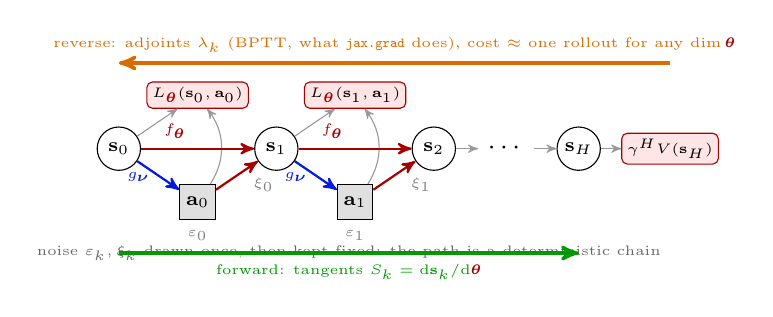
\begin{tikzpicture}[>=stealth', x=0.8cm, y=0.68cm,
  st/.style={circle, draw, fill=white, inner sep=0pt, minimum size=0.55cm, font=\scriptsize},
  ac/.style={rectangle, draw, fill=black!12, inner sep=1pt, minimum size=0.45cm, font=\scriptsize},
  co/.style={rectangle, rounded corners=2pt, draw=myRed2, fill=myLightRed, inner sep=2pt, font=\tiny},
  nz/.style={font=\tiny, text=black!50}]
% step 1: the policy acts, a_0 = g_nu(s_0, eps_0)
\node[st] (s0) at (0,0) {$\sv_0$};
\node[ac] (a0) at (1.25,-1.0) {$\av_0$};
\draw[->, myBlue3, thick] (s0) -- node[left, font=\tiny, pos=0.55]{$g_{\pnu}$} (a0);
\node[nz, anchor=north] at (a0.south) {$\varepsilon_0$};
% step 2: the cost
\node[co, visible on=<2->] (L0) at (1.25,1.0) {$\Lth(\sv_0,\av_0)$};
\draw[->, black!40, visible on=<2->] (s0) -- (L0);
\draw[->, black!40, visible on=<2->] (a0) to[bend right=35] (L0);
% step 3: the simulator, s_1 = f_theta(s_0, a_0, xi_0)
\node[st, visible on=<3->] (s1) at (2.5,0) {$\sv_1$};
\draw[->, myRed2, thick, visible on=<3->] (s0) -- node[above, font=\tiny, pos=0.3]{$f_{\mth}$} (s1);
\draw[->, myRed2, thick, visible on=<3->] (a0) -- (s1);
\node[nz, visible on=<3->] at (2.3,-0.68) {$\xi_0$};
% step 4: the same for k = 1
\node[ac, visible on=<4->] (a1) at (3.75,-1.0) {$\av_1$};
\draw[->, myBlue3, thick, visible on=<4->] (s1) -- node[left, font=\tiny, pos=0.55]{$g_{\pnu}$} (a1);
\node[nz, anchor=north, visible on=<4->] at (a1.south) {$\varepsilon_1$};
\node[co, visible on=<4->] (L1) at (3.75,1.0) {$\Lth(\sv_1,\av_1)$};
\draw[->, black!40, visible on=<4->] (s1) -- (L1);
\draw[->, black!40, visible on=<4->] (a1) to[bend right=35] (L1);
\node[st, visible on=<4->] (s2) at (5.0,0) {$\sv_2$};
\draw[->, myRed2, thick, visible on=<4->] (s1) -- node[above, font=\tiny, pos=0.3]{$f_{\mth}$} (s2);
\draw[->, myRed2, thick, visible on=<4->] (a1) -- (s2);
\node[nz, visible on=<4->] at (4.8,-0.68) {$\xi_1$};
% step 5: and so on, up to s_H
\node[visible on=<5->] (dots) at (6.15,0) {$\cdots$};
\node[st, visible on=<5->] (sH) at (7.3,0) {$\sv_H$};
\draw[->, black!40, visible on=<5->] (s2) -- (dots);
\draw[->, black!40, visible on=<5->] (dots) -- (sH);
\node[font=\tiny, text=black!60, visible on=<3-5>] at (3.65,-1.95) {noise $\varepsilon_k,\xi_k$ drawn once, then kept fixed: the path is a deterministic chain};
% step 8: a critic bootstraps the tail
\node[co, visible on=<12->] (V) at (8.75,0) {$\gamma^H V(\sv_H)$};
\draw[->, black!40, visible on=<12->] (sH) -- (V);
% forward tangent and reverse adjoint sweeps
\draw[visible on=<6->, ->, myGreen3, very thick] (0,-1.95) -- node[below, font=\tiny]{forward: tangents $S_k=\mathrm d\sv_k/\mathrm d\mth$} (7.3,-1.95);
\draw[visible on=<10->, <-, myOrangeD, very thick] (0,1.6) -- node[above, font=\tiny]{reverse: adjoints $\lambda_k$ (BPTT, what \texttt{jax.grad} does), cost $\approx$ one rollout for any $\dim\mth$} (8.75,1.6);
\end{tikzpicture}
\end{center}
\vspace{-.45cm}
\begin{columns}[T]
\column{0.53\textwidth}
\visible<6->{\textbf{Forward sensitivities} (one path, noise $\omega$ fixed)}
\begin{align*}
\visible<6->{A_k}&\visible<6->{= \nabla_{\sv} g_{\pnu}\,S_k,\qquad S_0=0}\\
\visible<7->{S_{k+1}}&\visible<7->{= \partial_{\mth} f_{\mth}+\nabla_{\sv}f_{\mth}\,S_k+\nabla_{\av}f_{\mth}\,A_k}\\
\visible<8->{\nabla_{\mth}\Jh}&\visible<8->{= \E_\omega\Big[\sum_k\gamma^k\big(\partial_{\mth}\Lth+\nabla_{\sv}\Lth\, S_k+\nabla_{\av}\Lth\, A_k\big)\Big]}
\end{align*}

\vspace{-.25cm}
\visible<9->{{\scriptsize For $\nabla_{\pnu}$: same recursion with $A_k=\nabla_{\sv}g_{\pnu}S_k+\nabla_{\pnu}g_{\pnu}$, no $\partial f$ term.}}
\column{0.45\textwidth}
\visible<11->{\textbf{Catch}: $S_k$ contains $\prod_i\nabla_{\sv}f_{\mth}$, which explodes or vanishes for long horizons, contacts, chaos}\\[3pt]
\visible<12->{\textbf{Fix} (SVG, SHAC): differentiate only $H$ steps and bootstrap the tail with a critic
\begin{align*}
\hat J_{H}=\E_\omega\big[\textstyle\sum_{k=0}^{H-1}\gamma^k\Lth(\sv_k,\av_k)+\gamma^H V(\sv_H)\big]
\end{align*}}
\end{columns}
\vspace{-.3cm}
\visible<13->{
{\scriptsize $\checkmark$ exact per-path gradients; low variance if the dynamics are smooth\\
\ding{56} needs differentiable $f_{\mth},g_{\pnu},\Lth$ (smooth surrogates for contact, $\min$, $\max$) and continuous $\av$, $\mth$}}
\end{frame}

%-----------------------------------------------------------------------
\begin{frame}{\normalsize Implicit differentiation of policy training}
\footnotesize
\begin{columns}[T]
\column{0.56\textwidth}
\textbf{A trained policy is a stationary point} of the in-sim objective
\begin{align*}
\Fres(\nst,\mth):=\nabla_{\pnu}\Jh(\nst)=0
\end{align*}

\vspace{-.3cm}
\visible<2->{{\scriptsize \LR: \ $\E\big[\sum_k\gamma^k\nabla_{\pnu}\log\pin\,Q^{\pin}_{\mth}\big]=0$ \hfill (PPO)\\
\PD: \ $\E_\omega\big[\sum_k\gamma^k\big(\nabla_{\sv}\Lth\,\tfrac{\mathrm d\sv_k}{\mathrm d\pnu}+\nabla_{\av}\Lth\,\tfrac{\mathrm d\av_k}{\mathrm d\pnu}\big)\big]=0$ \hfill (SVG)}}\\[3pt]
\visible<3->{\textbf{Assumptions}}
\begin{enumerate}
\scriptsize
\item<3-> \textbf{Smooth}: $\pin,\rth$ (\LR) or $g_{\pnu},f_{\mth}$ (\PD), and $\Lth$ are $C^2$
\item<4-> \textbf{$\nabla$ and $\E$ commute} (\LR: densities $>0$; \PD: integrable derivatives)
\item<5-> \textbf{Converged}: $\Fres(\nst,\mth)=0$; a \emph{local} optimum is enough
\item<6-> \textbf{Regular}: $\nst$ isolated, $A:=\nabla_{\pnu}\Fres$ nonsingular (e.g.\ $A\succ0$)
\item<7-> \textbf{Same spaces}: $\mth$ changes neither $\mathcal S$ nor $\mathcal A$
\end{enumerate}
\column{0.42\textwidth}
\begin{center}
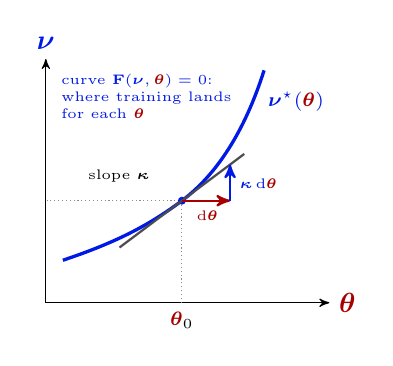
\begin{tikzpicture}[>=stealth', scale=0.72]
\draw[->] (0,0) -- (5.0,0) node[right]{$\mth$};
\draw[->] (0,0) -- (0,4.3) node[above]{$\pnu$};
\draw[myBlue3, very thick] (0.3,0.75) .. controls (1.2,1.05) and (1.8,1.35) .. (2.4,1.8) .. controls (3.0,2.25) and (3.5,3.0) .. (3.85,4.1);
\node[myBlue3, font=\scriptsize, anchor=west] at (3.75,3.55) {$\nst(\mth)$};
\node[myBlue3, font=\tiny, anchor=north west, align=left] at (0.1,4.2) {curve $\Fres(\pnu,\mth)=0$:\\where training lands\\for each $\mth$};
\draw[black!45, densely dotted] (2.4,0) -- (2.4,1.8) -- (0,1.8);
\node[font=\scriptsize, below] at (2.4,0) {$\mth_0$};
\fill[myBlue3] (2.4,1.8) circle (2pt);
\draw[visible on=<8->, black!70, thick] (1.3,0.975) -- (3.5,2.625);
\draw[visible on=<8->, ->, myRed2, thick] (2.4,1.8) -- (3.25,1.8);
\draw[visible on=<8->, ->, myBlue3, thick] (3.25,1.8) -- (3.25,2.4375);
\node[visible on=<8->, font=\tiny, below, text=myRed2] at (2.85,1.8) {$\mathrm d\mth$};
\node[visible on=<8->, font=\tiny, right, text=myBlue3] at (3.25,2.1) {$\kap\,\mathrm d\mth$};
\node[visible on=<8->, font=\tiny, anchor=south east] at (2.0,1.95) {slope $\kap$};
\end{tikzpicture}
\end{center}
\visible<9->{
{\scriptsize\textbf{Toy}: $\Jh(\pnu)=\frac a2\pnu^2-\mth\pnu$, \ so $\nst=\mth/a$\\
$\Fres=a\pnu-\mth$, \ $A=a$, \ $B=-1$\\
$\kap=-A^{-1}B=1/a$ \ $\checkmark$}}
\end{columns}
\vspace{-.25cm}
\visible<8->{
\begin{alertblock}{}
\textbf{IFT}: differentiate $\Fres\big(\nst(\mth),\mth\big)\equiv0$ \ $\Rightarrow$ \ $A\,\kap+B=0$ \ $\Rightarrow$ \ $\boxed{\kap=-A^{-1}B}$, \ \ $B:=\nabla_{\mth}\Fres$\\
{\scriptsize Only the \textbf{end point} of training matters: no unrolling, any policy class, any policy-gradient method.}
\end{alertblock}}
\end{frame}

%-----------------------------------------------------------------------
\begin{frame}{\normalsize Computing $A$ and $B$ for \LR\ policies (PPO, A2C)}
\footnotesize
\textbf{Recall}: $A=\nabla_{\pnu}\Fres$, \ $B=\nabla_{\mth}\Fres$, \ $\Fres=\E_{\tau\sim p_{\pnu,\mth}}\big[\sum_k\gamma^k\nabla_{\pnu}\log\pi_k\,Q_k\big]$: both the integrand ($Q_k$) and the \textbf{Markov chain} $p_{\pnu,\mth}$ depend on $(\pnu,\mth)$\\[4pt]
\begin{block}{\footnotesize The parameters act from three places \ (Anand et al., 2026, Theorem 1)}
$\pi_k=\pin(\av_k|\sv_k)$, \ $Q_k=Q^{\pin}_{\mth}(\sv_k,\av_k)$:
\begin{align*}
A&=\E\Big[\sum_k\gamma^k\Big(\underbrace{\nabla^2_{\pnu\pnu}\log\pi_k\,Q_k}_{\text{the node itself}}\visible<2->{{}+\underbrace{\nabla_{\pnu}\log\pi_k\,(\nabla_{\pnu}Q_k)^\top}_{\text{edges below (critic)}}}\visible<3->{{}+\underbrace{\nabla_{\pnu}\log\pi_k\,Q_k\,(W^{\pnu}_k)^\top}_{\text{edges above: the Markov chain}}}\Big)\Big]\\[4pt]
\visible<4->{B}&\visible<4->{=\E\Big[\sum_k\gamma^k\Big(\underbrace{\nabla_{\pnu}\log\pi_k\,(\nabla_{\mth}Q_k)^\top}_{\text{edges below (critic)}}+\underbrace{\nabla_{\pnu}\log\pi_k\,Q_k\,(W^{\mth}_k)^\top}_{\text{edges above: the Markov chain}}\Big)\Big]}
\end{align*}
\end{block}
\visible<5->{
\begin{itemize}
\item \textbf{Markov-chain sensitivity} (edges above): $W^{\pnu}_k=\sum_{i\le k}\nabla_{\pnu}\log\pi_i$, \ $W^{\mth}_k=\sum_{i\le k}\nabla_{\mth}\log\rho_{\mth,i}$
\item<6-> \textbf{Critic sensitivities} (edges below): $\nabla_{\pnu}Q_k$, $\nabla_{\mth}Q_k$, learned like a critic
\item<7-> \textbf{Only} $B$ differentiates in $\mth$: through the model edges $\rth$ and the costs $\Lth$ \ (PPO: $Q\to$ advantage)
\end{itemize}}
\vfill
\parbox{0.8\textwidth}{\tiny A.\,S.~Anand et al., \textit{Bi-Level Reinforcement Learning Pathway for Sim-to-Real Optimality}, RLC 2026.}
\end{frame}

%-----------------------------------------------------------------------
\begin{frame}{\normalsize Computing $A$ and $B$ for \PD\ policies (SVG)}
\footnotesize
\textbf{Recall}: the noise $\omega$ has a \textbf{fixed} distribution, so the Markov chain changes only by \textbf{moving the path} $z_k=(\sv_k,\av_k)$, smoothly in $(\pnu,\mth)$:
\begin{align*}
\Fres=\nabla_{\pnu}\Jh=\E_\omega\Big[\sum_k\gamma^k\,\nabla_{z}\Lth(z_k)\,Z^{\pnu}_k\Big],\qquad Z^{\pnu}_k=\frac{\mathrm dz_k}{\mathrm d\pnu},\quad Z^{\mth}_k=\frac{\mathrm dz_k}{\mathrm d\mth}\ \ \text{(forward sensitivities)}
\end{align*}
\visible<2->{\textbf{Differentiate once more along the same path} \ (A.S. Anand, 2026)}
\begin{align*}
\visible<2->{A}&\visible<2->{=\E_\omega\Big[\sum_k\gamma^k\Big(\underbrace{(Z^{\pnu}_k)^\top\nabla^2_{zz}\Lth\,Z^{\pnu}_k}_{\text{curvature of the cost}}+\underbrace{\nabla_z\Lth\,Z^{\pnu\pnu}_k}_{\text{curvature of the path}}\Big)\Big]}\\[4pt]
\visible<3->{B}&\visible<3->{=\E_\omega\Big[\sum_k\gamma^k\Big(\underbrace{(Z^{\pnu}_k)^\top\partial_{\mth}\nabla_z\Lth}_{\mth\text{ in the cost}}}\visible<4->{{}+\underbrace{(Z^{\pnu}_k)^\top\nabla^2_{zz}\Lth\,Z^{\mth}_k}_{\text{the path moves with }\mth}}\visible<5->{{}+\underbrace{\nabla_z\Lth\,Z^{\pnu\mth}_k}_{\mth\text{ bends the sensitivities}}}\visible<3->{\Big)\Big]}
\end{align*}
\visible<5->{{\scriptsize $Z^{\pnu\pnu}_k$, $Z^{\pnu\mth}_k$: second-order sensitivities; they bring in $\nabla^2 f_{\mth}$, \ $\nabla^2 g_{\pnu}$, \ $\partial_{\mth}\nabla f_{\mth}$}}
\begin{itemize}
\item<6-> $A\,v$ = \texttt{jvp} of $\Fres$, \ $B^\top w$ = \texttt{vjp} of $\Fres$ in $\mth$ \ (a few rollouts each)
\item<7-> \textbf{In practice} $A$ may be ill-conditioned or indefinite: use $A+\varepsilon I$ or a truncated eigendecomposition
\end{itemize}
\vfill
\parbox{0.8\textwidth}{\tiny A.\,S.~Anand et al., \textit{Gradient-Based Co-Design of Reinforcement Learning Policies with Differentiable Simulators}, TMLR 2026}
\end{frame}

%-----------------------------------------------------------------------
\begin{frame}{\normalsize Where do we use $\kap$? (1) Sim-to-real: tune the simulator}
\footnotesize
Motivation: a policy is trained in a simulator, then deployed on a real system.
\begin{center}
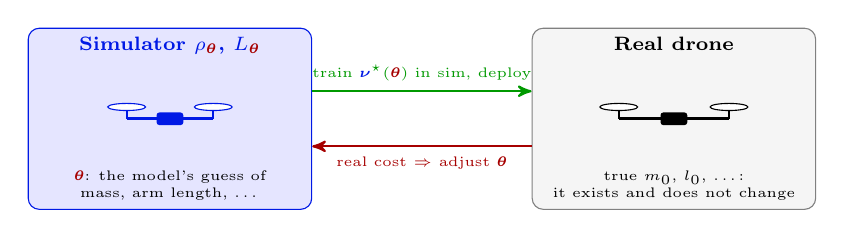
\begin{tikzpicture}[>=stealth', x=1cm, y=1cm]
\node[draw=myBlue3, fill=myLightBlue, rounded corners, minimum width=3.6cm, minimum height=2.3cm] (simp) at (0,0) {};
\node[font=\scriptsize\bfseries, text=myBlue3, anchor=north] at (simp.north) {Simulator $\rth$, $\Lth$};
\pic[myBlue3] at (0,0.0) {drone=0.55};
\node[font=\tiny, align=center, anchor=south] at (simp.south) {$\mth$: the model's guess of\\ mass, arm length, \dots};
\node[visible on=<2->, draw=black!50, fill=black!4, rounded corners, minimum width=3.6cm, minimum height=2.3cm] (realp) at (6.4,0) {};
\node[visible on=<2->, font=\scriptsize\bfseries, anchor=north] at (realp.north) {Real drone};
\pic[black, visible on=<2->] at (6.4,0.0) {drone=0.7};
\node[visible on=<2->, font=\tiny, align=center, anchor=south] at (realp.south) {true $m_0$, $l_0$, \dots:\\ it exists and does not change};
\draw[visible on=<2->, ->, thick, myGreen3] ($(simp.east)+(0,0.35)$) -- node[above, font=\tiny]{train $\nst(\mth)$ in sim, deploy} ($(realp.west)+(0,0.35)$);
\draw[visible on=<3->, <-, thick, myRed2] ($(simp.east)+(0,-0.35)$) -- node[below, font=\tiny]{real cost $\Rightarrow$ adjust $\mth$} ($(realp.west)+(0,-0.35)$);
\end{tikzpicture}
\end{center}
\begin{itemize}
\item<2-> Changing $\mth$ changes the \textbf{simulator}, our model of it
\item<3-> Goal: the policy trained in the simulator should do \textbf{best on the real robot}
\begin{align*}
\min_{\mth}\ \Jreal\big(\nst(\mth)\big),\qquad \nst(\mth)\ \text{trained in the simulator with parameters }\mth
\end{align*}
\item<4-> Not system identification: the best $\mth$ for \textbf{decisions} need not be the most accurate model 
\end{itemize}
\end{frame}

%-----------------------------------------------------------------------
\begin{frame}{\normalsize Where do we use $\kap$? (2) Co-design: design the system and its policy}
\footnotesize
The system is \textbf{to be designed}: $\mth$ as the \textbf{design space} (arm length, motor size; battery size, \dots)
\begin{center}
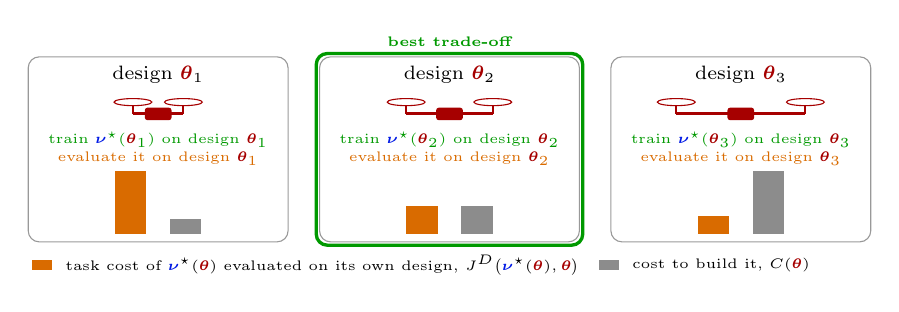
\begin{tikzpicture}[>=stealth', x=1cm, y=1cm]
\foreach \i/\x/\l/\tc/\bc in {1/0/0.32/0.8/0.2, 2/3.7/0.55/0.36/0.36, 3/7.4/0.82/0.24/0.8}{
  \node[draw=black!40, rounded corners, minimum width=3.3cm, minimum height=2.35cm] (p\i) at (\x,0) {};
  \node[font=\scriptsize, anchor=north] at (p\i.north) {design $\mth_{\i}$};
  \pic[myRed2] at (\x,0.45) {drone=\l};
  \node[visible on=<2->, font=\tiny, text=myGreen3] at (\x,0.12) {train $\nst(\mth_{\i})$ on design $\mth_{\i}$};
  \node[visible on=<3->, font=\tiny, text=myOrangeD] at (\x,-0.12) {evaluate it on design $\mth_{\i}$};
  \fill[visible on=<3->, myOrangeD] (\x-0.55,-1.08) rectangle ++(0.4,\tc);
  \fill[visible on=<4->, black!45] (\x+0.15,-1.08) rectangle ++(0.4,\bc);
}
\node[visible on=<5->, draw=myGreen3, very thick, rounded corners, fit=(p2), inner sep=1pt] {};
\node[visible on=<5->, font=\tiny\bfseries, text=myGreen3, anchor=south] at (p2.north) {best trade-off};
\fill[visible on=<3->, myOrangeD] (-1.6,-1.53) rectangle ++(0.25,0.12);
\node[visible on=<3->, font=\tiny, anchor=west] at (-1.3,-1.47) {task cost of $\nst(\mth)$ evaluated on its own design, $J^D\big(\nst(\mth),\mth\big)$};
\fill[visible on=<4->, black!45] (5.6,-1.53) rectangle ++(0.25,0.12);
\node[visible on=<4->, font=\tiny, anchor=west] at (5.9,-1.47) {cost to build it, $C(\mth)$};
\end{tikzpicture}
\end{center}
\vspace{-.2cm}
\begin{itemize}
\item<2-> Changing $\mth$ changes the \textbf{real system} itself, hence its MDP: the policy must be \textbf{re-trained}, $\nst(\mth)$
\item<3-> Each trained policy is \textbf{evaluated on its own design}: the system it is judged on changes with $\mth$ \ldots
\item<4-> \ldots\ plus what it costs to build: \quad $\min_{\mth}\ J^D\big(\nst(\mth),\mth\big)+C(\mth)$
\end{itemize}
\visible<5->{
\begin{alertblock}{}
\centering Sim-to-real: $\mth$ changes only the \textbf{model}. \qquad Co-design: $\mth$ changes the \textbf{robot itself}.
\end{alertblock}}
\end{frame}

%-----------------------------------------------------------------------
\begin{frame}{\normalsize Where is the trained policy evaluated?}
\footnotesize
\begin{center}
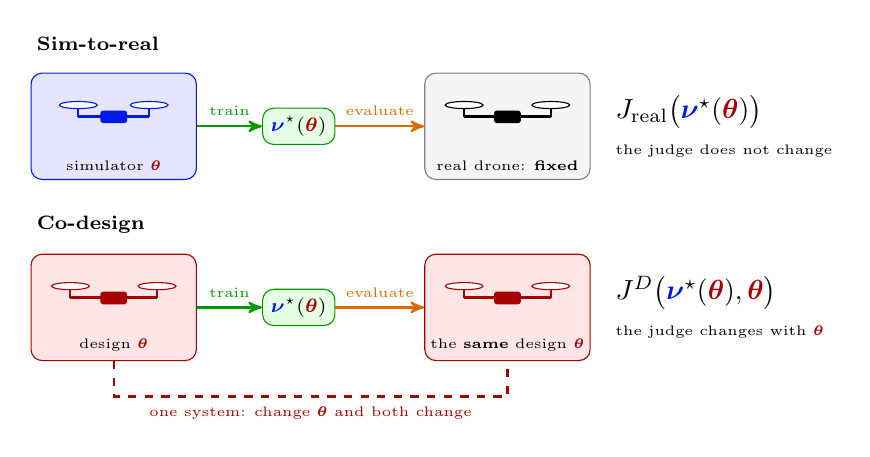
\begin{tikzpicture}[>=stealth', x=1cm, y=1cm,
  bx/.style={rounded corners, minimum width=2.1cm, minimum height=1.35cm},
  pol/.style={draw=myGreen3, fill=myLightGreen, rounded corners, inner sep=3pt, font=\scriptsize},
  capt/.style={font=\tiny, anchor=south}]
% ---- sim-to-real
\node[font=\scriptsize\bfseries, anchor=west] at (-0.1,1.05) {Sim-to-real};
\node[bx, draw=myBlue3, fill=myLightBlue] (s1) at (1,0) {};
\pic[myBlue3] at (1,0.12) {drone=0.45};
\node[capt] at (s1.south) {simulator $\mth$};
\node[pol] (n1) at (3.35,0) {$\nst(\mth)$};
\draw[->, thick, myGreen3] (s1) -- node[above, font=\tiny]{train} (n1);
\node[visible on=<2->, bx, draw=black!50, fill=black!4] (r1) at (6.0,0) {};
\pic[black, visible on=<2->] at (6.0,0.12) {drone=0.55};
\node[visible on=<2->, capt] at (r1.south) {real drone: \textbf{fixed}};
\draw[visible on=<2->, ->, thick, myOrangeD] (n1) -- node[above, font=\tiny]{evaluate} (r1);
\node[visible on=<2->, anchor=west, align=left] at (7.25,0) {$\Jreal\big(\nst(\mth)\big)$\\[1pt] {\tiny the judge does not change}};
% ---- co-design
\node[visible on=<3->, font=\scriptsize\bfseries, anchor=west] at (-0.1,-1.25) {Co-design};
\node[visible on=<3->, bx, draw=myRed2, fill=myLightRed] (s2) at (1,-2.3) {};
\pic[myRed2, visible on=<3->] at (1,-2.18) {drone=0.55};
\node[visible on=<3->, capt] at (s2.south) {design $\mth$};
\node[visible on=<3->, pol] (n2) at (3.35,-2.3) {$\nst(\mth)$};
\draw[visible on=<3->, ->, thick, myGreen3] (s2) -- node[above, font=\tiny]{train} (n2);
\node[visible on=<4->, bx, draw=myRed2, fill=myLightRed] (r2) at (6.0,-2.3) {};
\pic[myRed2, visible on=<4->] at (6.0,-2.18) {drone=0.55};
\node[visible on=<4->, capt] at (r2.south) {the \textbf{same} design $\mth$};
\draw[visible on=<4->, ->, thick, myOrangeD] (n2) -- node[above, font=\tiny]{evaluate} (r2);
\node[visible on=<4->, anchor=west, align=left] at (7.25,-2.3) {$J^D\big(\nst(\mth),\mth\big)$\\[1pt] {\tiny the judge changes with $\mth$}};
\draw[visible on=<4->, dashed, myRed2, thick] (s2.south) -- ++(0,-0.45) -| node[pos=0.25, below, font=\tiny]{one system: change $\mth$ and both change} (r2.south);
\end{tikzpicture}
\end{center}
\visible<5->{
\begin{center}
\renewcommand{\arraystretch}{1.5}
\begin{tabular}{lll}
sim-to-real: & $\Jreal\big(\nst(\mth)\big)$ & $\mth$ acts only through the \textbf{policy}\\
co-design: & $J^D\big(\nst(\mth),\mth\big)$ & $\mth$ acts through the \textbf{policy} \emph{and} the \textbf{evaluating system}
\end{tabular}
\end{center}}
\visible<6->{
\begin{alertblock}{}
\centering Co-design: $\mth$ acts \textbf{twice}, through the re-trained policy \emph{and} the system that evaluates it.\\
So only co-design has a \textbf{direct} term $\partial_{\mth}J^D$ (policy fixed, system changed).
\end{alertblock}}
\end{frame}

%-----------------------------------------------------------------------
\begin{frame}{\normalsize Using $\kap$: the gradient of the outer objective}
\footnotesize
\textbf{In both problems} we tune $\mth$ with the gradient of an \textbf{outer objective} $J^{\mathrm{out}}\big(\nst(\mth),\mth\big)$ that \textbf{judges} the trained policy. The blocker of slide 13 was $\nabla_{\mth}\pi_{\mth}=\nabla_{\pnu}\pin\,\kap$: now computable.
\vspace{-.1cm}
\begin{align*}
\nabla_{\mth}J^{\mathrm{out}}\big(\nst(\mth),\mth\big)=\underbrace{\partial_{\mth}J^{\mathrm{out}}}_{\text{direct: }\pnu\text{ fixed}}+\underbrace{\nabla_{\pnu}J^{\mathrm{out}}\,\kap}_{\text{indirect: the policy re-adapts}},\qquad \kap=-A^{-1}B
\end{align*}
\begin{center}
\scriptsize
\renewcommand{\arraystretch}{1.4}
\begin{tabular}{l|l|l}
 & \textbf{Sim-to-real} & \textbf{Co-design}\\ \hline
\uncover<2->{$\mth$} & \uncover<2->{simulator parameters} & \uncover<2->{design of the system}\\
\uncover<3->{$J^{\mathrm{out}}$} & \uncover<3->{$\Jreal(\nst)$, on the real robot} & \uncover<3->{$J^D(\nst,\mth)+C(\mth)$, in the simulator}\\
\uncover<4->{direct term} & \uncover<4->{$0$ (the real robot ignores $\mth$)} & \uncover<4->{$\neq0$ ($\mth$ changes the system)}\\
\uncover<5->{$\nabla_{\pnu}J^{\mathrm{out}}$} & \uncover<5->{\LR, from real rollouts} & \uncover<5->{\PD\ (AD), in the simulator}\\
\end{tabular}
\end{center}
\visible<6->{
\textbf{Adjoint trick} (never form $\kap$): with $g=\nabla_{\pnu}J^{\mathrm{out}}$, \ $g^\top\kap=-g^\top A^{-1}B$, so
\begin{enumerate}
\scriptsize
\item solve $A^\top\lambda=g$: one matrix-free linear solve in $\dim\pnu$ (CG, MINRES, GMRES)
\item<7-> indirect term $=-B^\top\lambda$: one vector--Jacobian product ($>100\times$ faster)
\end{enumerate}}
\end{frame}

%-----------------------------------------------------------------------
% \begin{frame}[fragile]{\normalsize Practical implementation in JAX: (almost) all automatic differentiation}
% \footnotesize
% \begin{columns}[T]
% \column{0.58\textwidth}
% {\tiny
% \begin{semiverbatim}
% import jax
% from jax.scipy.sparse.linalg import gmres

% {\color{gray}# J_sim(nu, theta, key): in-sim training objective}
% {\color{gray}#   PD: plain rollout, fixed noise from key}
% {\color{gray}#   LR: score-function (DiCE) surrogate, see below}
% def F(nu, theta, key):           {\color{gray}# stationarity residual}
%     return jax.grad(J_sim)(nu, theta, key)

% \uncover<2->{def indirect(nu, theta, key, g, eps=1e-3):
%     {\color{gray}# g = dJ_real/dnu at the trained nu = nu*(theta)}
%     _, AT = jax.vjp(lambda n: F(n, theta, key), nu)
%     lam, _ = gmres(lambda v: AT(v)[0] + eps * v, g)
%     _, BT = jax.vjp(lambda t: F(nu, t, key), theta)
%     return -BT(lam)[0]           {\color{gray}# = kappa^T g}}

% \uncover<3->{{\color{gray}# co-design (PD): total design gradient}
% g_dir = jax.grad(J_D, argnums=1)(nu, theta, key)
% g_nu  = jax.grad(J_D, argnums=0)(nu, theta, key)
% grad  = (g_dir + indirect(nu, theta, key, g_nu)
%          + jax.grad(C)(theta))}

% \uncover<4->{{\color{gray}# sim-to-real (LR): g from real rollouts, no g_dir}
% grad  = indirect(nu, theta, key, g_real)}
% \end{semiverbatim}}
% \column{0.4\textwidth}
% \scriptsize
% \renewcommand{\arraystretch}{1.15}
% \begin{tabular}{@{}ll@{}}
% \hline
% object & JAX\\
% \hline
% $\Fres=\nabla_{\pnu}\Jh$ & \texttt{grad}\\
% \uncover<2->{$A\,v$ \ (\PD: a Hessian)} & \uncover<2->{\texttt{jvp} of $\Fres$}\\
% \uncover<2->{$A^\top v$, \ $B^\top v$} & \uncover<2->{\texttt{vjp} of $\Fres$}\\
% \uncover<2->{$A^{-\top}g$} & \uncover<2->{\texttt{cg}, \texttt{gmres}}\\
% \uncover<2->{$\kap^\top g$} & \uncover<2->{1 solve $+$ 1 \texttt{vjp}}\\
% \uncover<3->{direct term} & \uncover<3->{\texttt{grad} in $\mth$}\\
% \hline
% \end{tabular}
% \begin{itemize}
% \item<5-> same \texttt{key} (noise) in every term
% \item<6-> \texttt{jit} $+$ \texttt{vmap} over parallel environments
% \item<7-> flatten $\pnu,\mth$ with \texttt{ravel\_pytree}
% \item<8-> \PD: $A$ is symmetric, so use \texttt{jvp} (forward-over-reverse) and CG or MINRES
% \end{itemize}
% \end{columns}
% \visible<9->{
% \begin{alertblock}{}
% \scriptsize \textbf{\LR\ caveat}: \texttt{grad} of a plain Monte-Carlo average treats the samples as fixed and drops every score term. Use a surrogate whose 1st \emph{and} 2nd derivatives are the \LR\ estimators, e.g.\ DiCE (Foerster et al., 2018):
% $\Jh\approx\sum_k\gamma^k\,\boxdot(W_k)\,\Lth(\sv_k,\av_k)$, \ $\boxdot(W)=e^{\,W-\texttt{stop\_gradient}(W)}=1$, \ $W_k$ = sum of the $\log\pin$, $\log\rth$ terms up to step $k$ (the running score)
% \end{alertblock}}
% \end{frame}

%%%%%%%%%%%%%%%%%%%%%%%%%%%%%%%%%%%%%%%%%%%%%%%%%%%%%%%%%%%%%%%%%%%%%%%%
\section{Examples}

%-----------------------------------------------------------------------
\begin{frame}{\normalsize Example 1: Sim-to-real RL (and Dyna-style MBRL)}
\footnotesize
\tikzstyle{Sys_block} = [rectangle, draw, fill=none, text width=2.3cm, text centered, rounded corners, inner sep=2pt]
\tikzstyle{Opt_block} = [rectangle, draw, fill=myLightGreen, text width=2.0cm, text centered, rounded corners, inner sep=3pt]
\tikzstyle{ID_block} = [rectangle, draw, fill=myLightBlue, text width=2.0cm, text centered, rounded corners, inner sep=3pt]
\tikzstyle{Out_block} = [rectangle, draw, fill=myLightRed, text width=2.3cm, text centered, rounded corners, inner sep=3pt]
\begin{columns}[T]
\column{0.5\textwidth}
\begin{tikzpicture}[->,>=stealth', font=\scriptsize]
\node[ID_block] (sim) at (0,0) {\textbf{Simulator}\\ $\hat\sv_+\sim\rth(\cdot|\sv,\av)$\\ cost $\Lth$};
\node[Opt_block] (pol) at (0,-2.2) {\textbf{In-sim PPO}\\ $\pnu\to\nst(\mth)$};
\node[Sys_block] (real) at (3.25,-2.3) {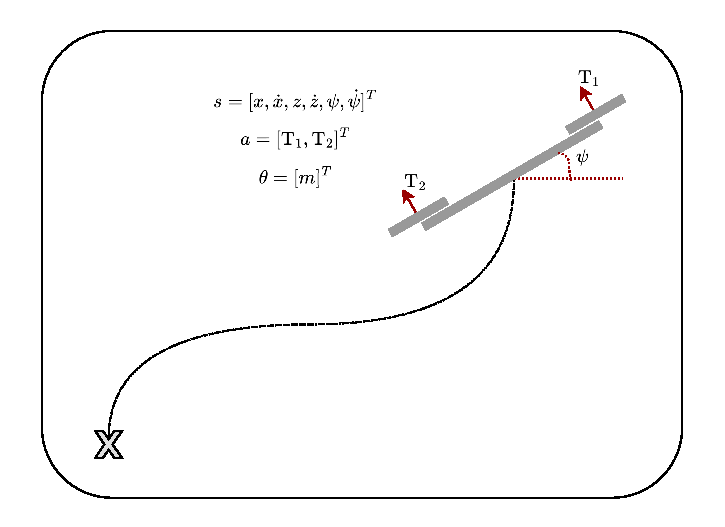
\includegraphics[width=1.9cm]{RLRL/quad2d_task.pdf}\\[-1pt] \textbf{Real system} $\rho$, $L$};
\node[Out_block] (out) at (3.25,0.15) {\textbf{Real-world RL}\\ $\mth\leftarrow\mth-\alpha\,\kap^\top\hat g$};
\path (sim) edge[bend left=22] node[right]{data} (pol)
      (pol) edge[bend left=22] node[left]{$\av$} (sim)
      (pol.east) edge node[above, pos=0.4, font=\tiny]{deploy} (real.west |- pol.east)
      (real) edge node[right]{real data $\hat g$} (out)
      (out) edge node[above]{$\Delta\mth$} (sim);
\draw[myBlue3, dashed, thick] (pol.north east) to[bend right=12] node[pos=0.68, above left=0pt, font=\tiny, fill=white, inner sep=1pt]{$\kap$ (IFT)} ($(out.south west)!0.35!(out.south east)$);
\draw[blue, thick, -] ($(sim.north west)+(-0.15,0.15)$) rectangle ($(pol.south east)+(0.15,-0.15)$);
\node[font=\tiny, text=blue, anchor=north] at ($(pol.south)+(0,-0.15)$) {in-sim};
\end{tikzpicture}\\[2pt]
\visible<4->{{\scriptsize \textbf{Converges} almost surely on three timescales: critics \textbf{fast}, policy $\pnu$ \textbf{medium}, simulator $\mth$ \textbf{slow}}}
\column{0.48\textwidth}
{\scriptsize \textbf{Recall} (slide 26): tune the simulator $\mth$ so that the policy trained in it is best on the real robot.}\\[3pt]
\textbf{Bi-level RL}
\begin{align*}
\min_{\mth}&\quad \Jreal(\pi_{\nst}) = \E_{\rho,\,\pi_{\nst}}\Big[\sum_k\gamma^k L(\sv_k,\av_k)\Big]\\
\text{s.t.}&\quad \nabla_{\pnu}\Jh(\nst)=0
\end{align*}
\begin{itemize}
\item<2-> \textbf{In-sim}: standard RL in the simulator (PPO, \LR)
\item<3-> \textbf{Real world}: \LR\ policy gradient on real data using $\kap$
\end{itemize}
\end{columns}
\vspace{-.25cm}
\visible<5->{
\textbf{Remarks}
\begin{itemize}
\item Optimal $\mth$ are not unique: pick the most ``accurate'' one (fitting loss as regularizer)
\item \visible<6->{\textbf{Dyna-style MBRL}: $\rth$ is learned; the real-world gradient complements MLE}
\item \visible<7->{vs.\ fine-tuning $\pnu$ on hardware: $\mth$ is small, physical and explainable}
\end{itemize}}
\end{frame}

%-----------------------------------------------------------------------
\begin{frame}{\normalsize Bi-level PPO and a quadrotor example}
\footnotesize
\begin{columns}[T]
\column{0.54\textwidth}
\vspace{-.45cm}
\begin{algorithm}[H]
\scriptsize
\caption{\scriptsize Bi-level PPO (costs, minimization)}
\For{real-world iteration $j=1,2,\dots$}{
 \lFor{$N_{\rm in}$ steps}{PPO update of $\pnu$ in $\rth,\Lth$ (warm start)}
 Roll out $\pin$ in sim: estimate $A$, $B$\;
 Roll out $\pin$ on the real system: $\hat g=\nabla_{\pnu}J$\;
 Solve $(A^\top+\varepsilon I)\,\lambda=\hat g$\;
 $\mth\leftarrow\mth+\alpha\,B^\top\lambda$ \tcp*{$=\mth-\alpha\kap^\top\hat g$}
}
\end{algorithm}
\column{0.44\textwidth}
\begin{overlayarea}{\textwidth}{0.4\textheight}
\only<1-4>{
\textbf{2D quadrotor} (safe-control-gym): reach a goal from random initial states
\begin{itemize}
\item<2-> simulator intialized with wrong (mass, length)
\item<3-> policy and critics: neural networks
\end{itemize}}
\only<4->{
\begin{itemize}
\item<5-> in-sim policy (red dotted) misses the goal: the sim-to-real gap
\item<6-> bi-level PPO closes the gap
\item<7-> \textbf{mass $\to\approx0.85\,m_0$}: wrong model, optimal policy
\end{itemize}}
\end{overlayarea}
\end{columns}
\vspace{-.2cm}
\visible<5->{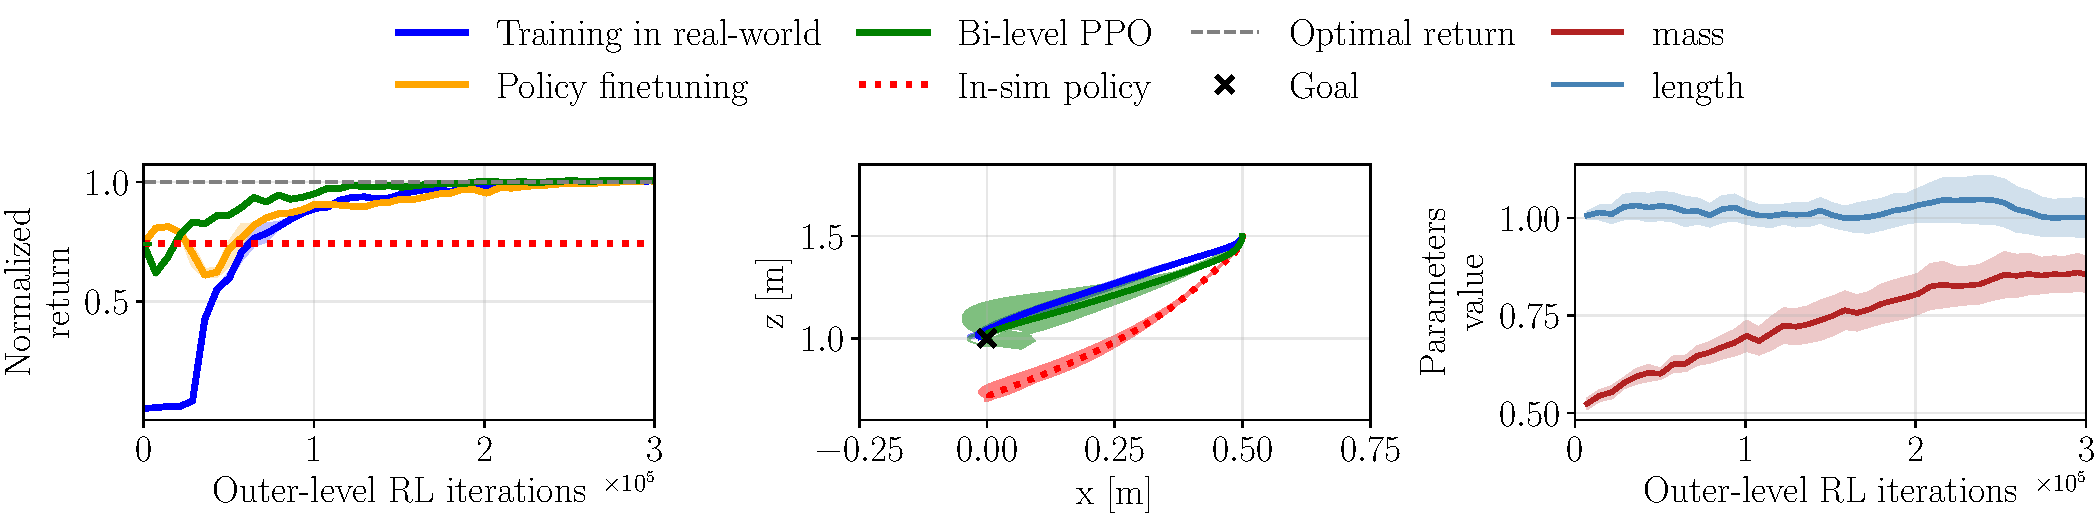
\includegraphics[width=\textwidth]{Figures/SimToReal/quadcopter.pdf}}
\end{frame}

%-----------------------------------------------------------------------
\begin{frame}{\normalsize Example 2: Co-design of a system and its policy}
\footnotesize
\begin{columns}[T]
\column{0.5\textwidth}
{\scriptsize \textbf{Recall} (slide 27): $\mth$ is the design; each design needs its own trained policy.}\\[3pt]
\textbf{Bi-level problem}
\begin{align*}
\min_{\mth}&\quad J^{D}\big(\nst(\mth),\mth\big)+C(\mth)\\
\text{s.t.}&\quad \nst(\mth)\in\argmin_{\pnu}J^{\pi}(\pnu,\mth)
\end{align*}
\begin{itemize}
\item<2-> $J^\pi$: \textbf{operational} cost, trains the policy in-sim (the role of $\Jh$)
\item<3-> $J^D$ \textbf{judges} the design (the role of $J^{\mathrm{out}}$), $C(\mth)$: cost to build it
\item<4-> Usual practice: Bayesian optimization (BO) or evolution strategies (ES) around full RL runs; scales poorly with $\dim\mth$
\item<5-> Here: differentiable simulator, so \PD\ everywhere
\end{itemize}
\column{0.48\textwidth}
\visible<6->{
\textbf{Example: inventory--routing network}\\
{\scriptsize instead of a drone: $\mth$ = capacities, not arm lengths}
\begin{center}
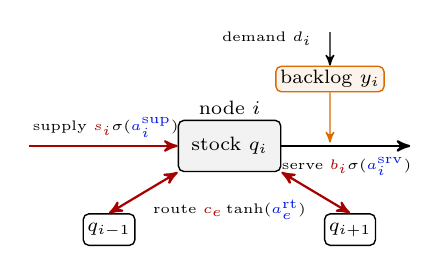
\begin{tikzpicture}[>=stealth', line width=0.5pt, scale=0.85,
  every node/.style={font=\tiny, inner sep=1.5pt}]
\node[draw, rounded corners=2pt, fill=black!5, minimum width=1.3cm, minimum height=0.65cm, font=\scriptsize] (nd) at (0,0) {stock $q_i$};
\node[anchor=south, font=\scriptsize] at (nd.north) {node $i$};
\draw[->, thick, myRed2] (-3.0,0) -- (nd.west);
\node[anchor=south] at (-1.85,0.05) {supply $\textcolor{myRed2}{s_i}\sigma(\textcolor{myBlue3}{a^{\rm sup}_i})$};
\draw[->, thick] (nd.east) -- (2.7,0);
\node[anchor=north] at (1.75,-0.1) {serve $\textcolor{myRed2}{b_i}\sigma(\textcolor{myBlue3}{a^{\rm srv}_i})$};
\node[draw=myOrangeD, rounded corners=2pt, fill=myOrangeD!8, font=\scriptsize] (bl) at (1.5,1.0) {backlog $y_i$};
\draw[->] (1.5,1.7) -- (bl.north);
\node[anchor=east] at (1.3,1.6) {demand $d_i$};
\draw[->, myOrangeD] (bl.south) -- (1.5,0.05);
\node[draw, rounded corners=2pt, minimum height=0.4cm, font=\scriptsize] (jm) at (-1.8,-1.25) {$q_{i-1}$};
\node[draw, rounded corners=2pt, minimum height=0.4cm, font=\scriptsize] (jp) at (1.8,-1.25) {$q_{i+1}$};
\draw[<->, thick, myRed2] (jm.north) -- (nd.south west);
\draw[<->, thick, myRed2] (jp.north) -- (nd.south east);
\node at (0,-0.95) {route $\textcolor{myRed2}{c_e}\tanh(\textcolor{myBlue3}{a^{\rm rt}_e})$};
\end{tikzpicture}
\end{center}
\scriptsize
\begin{itemize}
\item state: stock $q_i$, backlog $y_i$, AR(1) demand $d_i$
\item<7-> $\mth$: \textcolor{myRed2}{supply, service, routing capacities}, $\dim\mth$ from $15$ to $150$
\item<8-> the design bounds the \textcolor{myBlue3}{actions}; softplus-smoothed $\min,\max$
\item<9-> $J^D=J^\pi+\lambda_y\cdot$\textcolor{myOrangeD}{backlog}, \ $C(\mth)$ quadratic
\end{itemize}}
\end{columns}
\end{frame}

%-----------------------------------------------------------------------
\begin{frame}{\normalsize Co-design gradient with pathwise (SVG) in-sim training}
\footnotesize
\begin{columns}[T]
\column{0.58\textwidth}
\begin{align*}
\nabla_{\mth}\big(J^D+C\big)=\underbrace{\textcolor{myOrangeD}{\partial_{\mth}J^D}}_{\text{direct}}+\underbrace{\textcolor{myBlue3}{\nabla_{\pnu}J^D\,\kap}}_{\text{indirect}}+\nabla_{\mth}C
\end{align*}
\visible<3->{\textbf{Along a sampled path}, $\kap$ enters through the actions:}
\begin{align*}
\visible<3->{A_k}&\visible<3->{=\nabla_{\sv}g_{\pnu}\,S_k+\nabla_{\pnu}g_{\pnu}\,\kap}\\
\visible<3->{S_{k+1}}&\visible<3->{=\partial_{\mth}f_{\mth}+\nabla_{\sv}f_{\mth}\,S_k+\nabla_{\av}f_{\mth}\,A_k}
\end{align*}

\vspace{-.2cm}
\visible<4->{
\textbf{Envelope}: indirect term $=0$ if $J^D=J^\pi$; the backlog penalty ($\lambda_y>0$) makes $J^D\neq J^\pi$.}
\column{0.4\textwidth}
\visible<2->{
\begin{center}
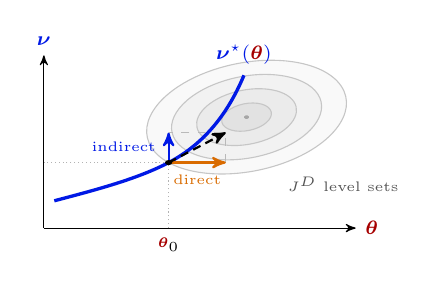
\begin{tikzpicture}[>=stealth', yscale=0.7, scale=0.66]
\begin{scope}[shift={(3.9,3.05)}, rotate=25]
  \foreach \r/\shade in {2.0109/5, 1.51/10, 1.005/16, 0.50/23}
    \filldraw[fill=gray!\shade, draw=gray!45, line width=0.4pt] (0,0) ellipse ({\r} and {0.72*\r});
  \fill[gray!70] (0,0) circle (1.4pt);
\end{scope}
\node[gray!65!black, font=\tiny, anchor=west] at (4.5,1.2) {$J^{D}$ level sets};
\draw[->] (0,0)--(6.0,0) node[right, font=\scriptsize] {$\mth$};
\draw[->] (0,0)--(0,4.75) node[above, font=\scriptsize] {$\pnu$};
\draw[gray!60, densely dotted] (2.4,0)--(2.4,1.8)--(0,1.8);
\node[font=\tiny, below] at (2.4,0) {$\mth_0$};
\draw[myBlue3, very thick] (0.2,0.75) .. controls (1.0,1.05) and (1.8,1.35) .. (2.4,1.8) .. controls (3.0,2.25) and (3.5,3.0) .. (3.85,4.2);
\node[text=myBlue3, font=\scriptsize, anchor=south] at (3.85,4.22) {$\nst(\mth)$};
\draw[gray!55, dashed, line width=0.4pt] (3.5,1.8)--(3.5,2.625)--(2.4,2.625);
\draw[->, myOrangeD, thick] (2.4,1.8) -- (3.5,1.8);
\draw[->, myBlue3, thick] (2.4,1.8) -- (2.4,2.625);
\draw[->, densely dashed, thick] (2.4,1.8) -- (3.5,2.625);
\fill (2.4,1.8) circle (2pt);
\node[text=myOrangeD, font=\tiny, anchor=north] at (2.95,1.74) {direct};
\node[text=myBlue3, font=\tiny, anchor=east] at (2.34,2.25) {indirect};
\end{tikzpicture}
\end{center}
{\scriptsize A design step $=$ a move at fixed policy $+$ the induced policy shift along $\nst(\mth)$}}
\end{columns}
\visible<5->{
\begin{algorithm}[H]
\scriptsize
\caption{\scriptsize Gradient-based co-design (costs, minimization)}
\For{$k=0,1,2,\dots$}{
 A few warm-started SVG steps on $J^\pi(\cdot,\mth_k)$: they only have to \textbf{track} $\nst(\mth_k)$\;
 $g_{\rm dir}\leftarrow\partial_{\mth}J^D$, \ one \texttt{jax.grad} with $\pnu$ fixed\;
 \lIf{$J^D\neq J^\pi$}{$u\leftarrow\nabla_{\pnu}J^D$, \ $g_{\rm ind}\leftarrow-B^\top(A+\varepsilon I)^{-1}u$; \ \textbf{else} $g_{\rm ind}\leftarrow0$}
 $\mth_{k+1}\leftarrow\Pi_\Theta\big(\mth_k-\alpha\,(g_{\rm dir}+g_{\rm ind}+\nabla_{\mth}C)\big)$\;
}
\end{algorithm}}
\visible<6->{{\scriptsize \textbf{Converges} to an approximately stationary design for small $\alpha$: \ error $\mathcal O\big(\tfrac1{\alpha N}\big)+\mathcal O(\alpha\sigma^2)+$ bias}}
\end{frame}

%-----------------------------------------------------------------------
\begin{frame}{\normalsize Co-design results: inventory--routing network}
\footnotesize
\begin{overlayarea}{\textwidth}{0.86\textheight}
\only<1-3>{
\textbf{Against black-box search}: 100 design evaluations each, matched objectives ($\lambda_y=0$, so the $\kap$-term is $0$ and only the direct gradient is used)
\begin{center}
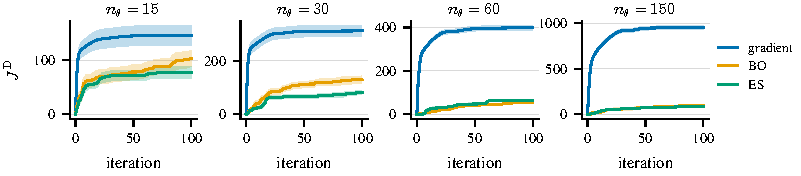
\includegraphics[width=\textwidth]{Figures/CoDesign/fig_benchmark.pdf}
\end{center}
\begin{itemize}
\item<2-> the gradient approach outperforms BO and ES at every size, and the gap grows with $\dim\mth$ ($15$ to $150$)
\item<3-> cost per design evaluation: $\approx2$\,s for the gradient, $\approx2$\,s ES, $\approx3$\,s BO
\end{itemize}}
\only<4->{
\textbf{Effect of the $\kap$-term}: mismatched objectives ($\lambda_y=0.1$, $J^D\neq J^\pi$)
\begin{center}
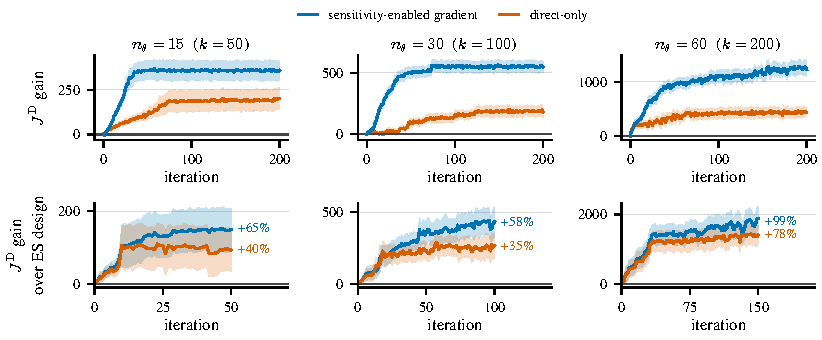
\includegraphics[width=0.82\textwidth]{Figures/CoDesign/fig_effect_refinement.pdf}
\end{center}
\vspace{-.2cm}
\begin{itemize}
\item<5-> \textbf{top}: sensitivity-enabled vs direct-only gradient, from the same initial design: the $\kap$-term helps, more in higher dimension
\item<6-> \textbf{bottom}: starting from the best design of a converged ES search: the gradient still improves it
\item<7-> cost: $\approx6.5$\,s per design evaluation with a matrix-free $\kap$-solve (vs $\approx2$\,s direct-only)
\end{itemize}}
\end{overlayarea}
\vspace{-.5cm}
{\tiny Plots show the design \emph{return} $-(J^D+C)$: higher is better.}
\end{frame}

%-----------------------------------------------------------------------
% \begin{frame}{\normalsize Convergence: does in-sim training have to converge?}
% \footnotesize
% \begin{columns}[T]
% \column{0.48\textwidth}
% \begin{block}{\footnotesize Sim-to-real: bi-level SPG (\LR)}
% \textbf{Three timescales} (stochastic approximation):
% \begin{itemize}
% \item critics and sensitivity critics: \textbf{fast}
% \item<2-> in-sim policy $\pnu$: \textbf{medium}
% \item<3-> simulator $\mth$: \textbf{slow}
% \end{itemize}
% \visible<4->{{\scriptsize Robbins--Monro step sizes for each layer, with step-size ratios (slower/faster) $\to0$}}\\[4pt]
% \visible<5->{\textbf{Result}: almost surely $\pnu_j-\nst(\mth_j)\to0$ and $\mth_j$ converges to the stationary points of $\Jreal\big(\pi_{\nst(\mth)}\big)$}\\[3pt]
% \visible<5->{{\scriptsize Each layer sees the slower ones as frozen and the faster ones as converged (ODE method)}}
% \end{block}
% \column{0.5\textwidth}
% \visible<6->{
% \begin{block}{\footnotesize Co-design: nested, warm-started SVG (\PD)}
% After $N$ design updates with a small step $\alpha$:
% {\scriptsize
% \begin{align*}
% \frac1N\sum_{k<N}\E\big\|\nabla_{\mth}J^D(\mth_k)\big\|^2\le\ &\mathcal O\Big(\frac1{\alpha N}\Big)+\mathcal O(\alpha\sigma^2)\\
% &+\mathcal O\big(\bar e^{\,2}+\Lambda^2\delta_\kappa^2+\delta_H^2\big)
% \end{align*}}

% \vspace{-.25cm}
% \begin{itemize}
% \scriptsize
% \item<7-> first two terms: SGD on a smooth nonconvex objective
% \item<8-> $\bar e$: in-sim tracking error, shrinks with $\alpha$ (warm start)
% \item<9-> $\delta_\kappa$: damped-solve error, times $\Lambda=\sup\|\nabla_{\pnu}J^D(\nst)\|$, which is $0$ if $J^D=J^\pi$
% \item<10-> $\delta_H\propto\gamma^H$: error of the terminal critic
% \end{itemize}
% \end{block}}
% \end{columns}
% \visible<11->{
% \begin{alertblock}{}
% \center
% In-sim training only has to \textbf{track} $\nst(\mth)$, not converge at every $\mth$-update: small $\mth$-steps make $\nst(\mth)$ move slowly.
% Guarantees are \textbf{local} (stationary points) and rest on the IFT assumptions.
% \end{alertblock}}
% \end{frame}

%-----------------------------------------------------------------------
\begin{frame}{\normalsize Take-aways}
\footnotesize
\begin{enumerate}
\item<1-> A policy trained in a model is an \textbf{implicit function} of the MDP: $\nst(\mth)$
\item<2-> \textbf{Bellman tree}: $\pnu$ lives on the action edges, $\mth$ on the transition edges and the costs
\begin{itemize}
\scriptsize
\item \LR: an edge passes $\partial\log P(\text{edge})\times$(value below it): no derivatives in $(\sv,\av)$, real data; variance grows with $|Q|$
\item \PD: chain rule along each sampled path: differentiable simulators; low variance if the dynamics are smooth; $H$ steps $+$ critic
\end{itemize}
\item<3-> \textbf{IFT} on the stationarity of training: $\kap=-A^{-1}B$. Only the end point of training matters
\item<4-> \textbf{Outer gradient} $=$ direct $+$ $\nabla_{\pnu}J^{\mathrm{out}}\,\kap$: sim-to-real tunes the \emph{model} (direct $=0$), co-design the \emph{system} (both terms)
\item<5-> \textbf{In JAX}: \texttt{grad}, \texttt{jvp}, \texttt{vjp} $+$ one Krylov solve; never form $\kap$; \LR\ needs a DiCE-type surrogate
\item<6-> \textbf{Applications}: simulators tuned for \emph{decisions} (sim-to-real, MBRL) and system design (co-design)
\end{enumerate}
\visible<7->{
\textbf{Open questions}: scaling the critic sensitivities, conditioning of $A$ for deep networks, offline real-world updates, partial observability

\vspace{.15cm}
{\scriptsize
\textbf{Papers}
\begin{itemize}
\item Anand et al., \textit{Bi-level RL pathway for sim-to-real optimality}, RLC 2026
\item Anand et al., \textit{Gradient-based co-design of RL policies with differentiable simulators}, TMLR 2026
\end{itemize}}}
\end{frame}

\end{document}
